\documentclass[UTF8]{ctexart}
\title{汽车构造拆装实习报告}
\author{1852479 康嘉梁}
\date{}
\ctexset{
bibname = {参考文献},
}
\pagestyle{plain}

\usepackage[a4paper]{geometry}
\geometry{left=3.18cm,right=3.18cm,top=2.54cm,bottom=2.54cm}

\usepackage{amsmath}
\numberwithin{figure}{section}
\numberwithin{table}{section}

% \renewcommand\thesection{\chinese{section}}
% \renewcommand\thesubsection{\arabic{subsection}}
% \renewcommand\thesubsubsection{\thesubsection\thinspace.\thinspace\arabic{subsubsection}}

\usepackage[version=4]{mhchem}

\usepackage{siunitx}

\usepackage{cleveref}
\crefname{section}{节}{节}
\crefname{equation}{式}{式}
\crefname{figure}{图}{图}
\crefname{table}{表}{表}
\crefname{appendix}{附录}{附录}
\newcommand{\crefpairconjunction}{~和~}
\newcommand{\crefmiddleconjunction}{、}
\newcommand{\creflastconjunction}{~和~}
\newcommand{\crefpairgroupconjunction}{~和~}
\newcommand{\crefmiddlegroupconjunction}{、}
\newcommand{\creflastgroupconjunction}{~和~}
\newcommand{\crefrangeconjunction}{~}

\usepackage{graphicx}
\DeclareGraphicsExtensions{.pdf,.eps,.jpg,.png}
\graphicspath{{img/body}, {img/gearbox}}
\usepackage{caption}
\captionsetup[figure]{labelsep=period}
\usepackage{float} %设置图片浮动位置的宏包
\usepackage{subfigure} %插入多图时用子图显示的宏包

\begin{document}
\maketitle

\section{车身部分}
\subsection{请简述从发动机排气歧管到车辆排气口,由哪些主要部分组成。各部分的主要功能是什么?}

\label{subsection:1.1}

对于实验室中的领克02来说,从发动机排气歧管排出的尾气经排气管、涡轮机(\cref{turbine})、三元催化转换器及颗粒捕集器(\cref{three-way catalytic converter})、前消声器(\cref{muffler F})、后消声器(\cref{muffler B}),最后由左右两个排气尾管(\cref{tail pipe})排到大气中。

\begin{figure}[htbp]
	\centering
	\begin{minipage}[b]{0.3\textwidth}
		\centering
		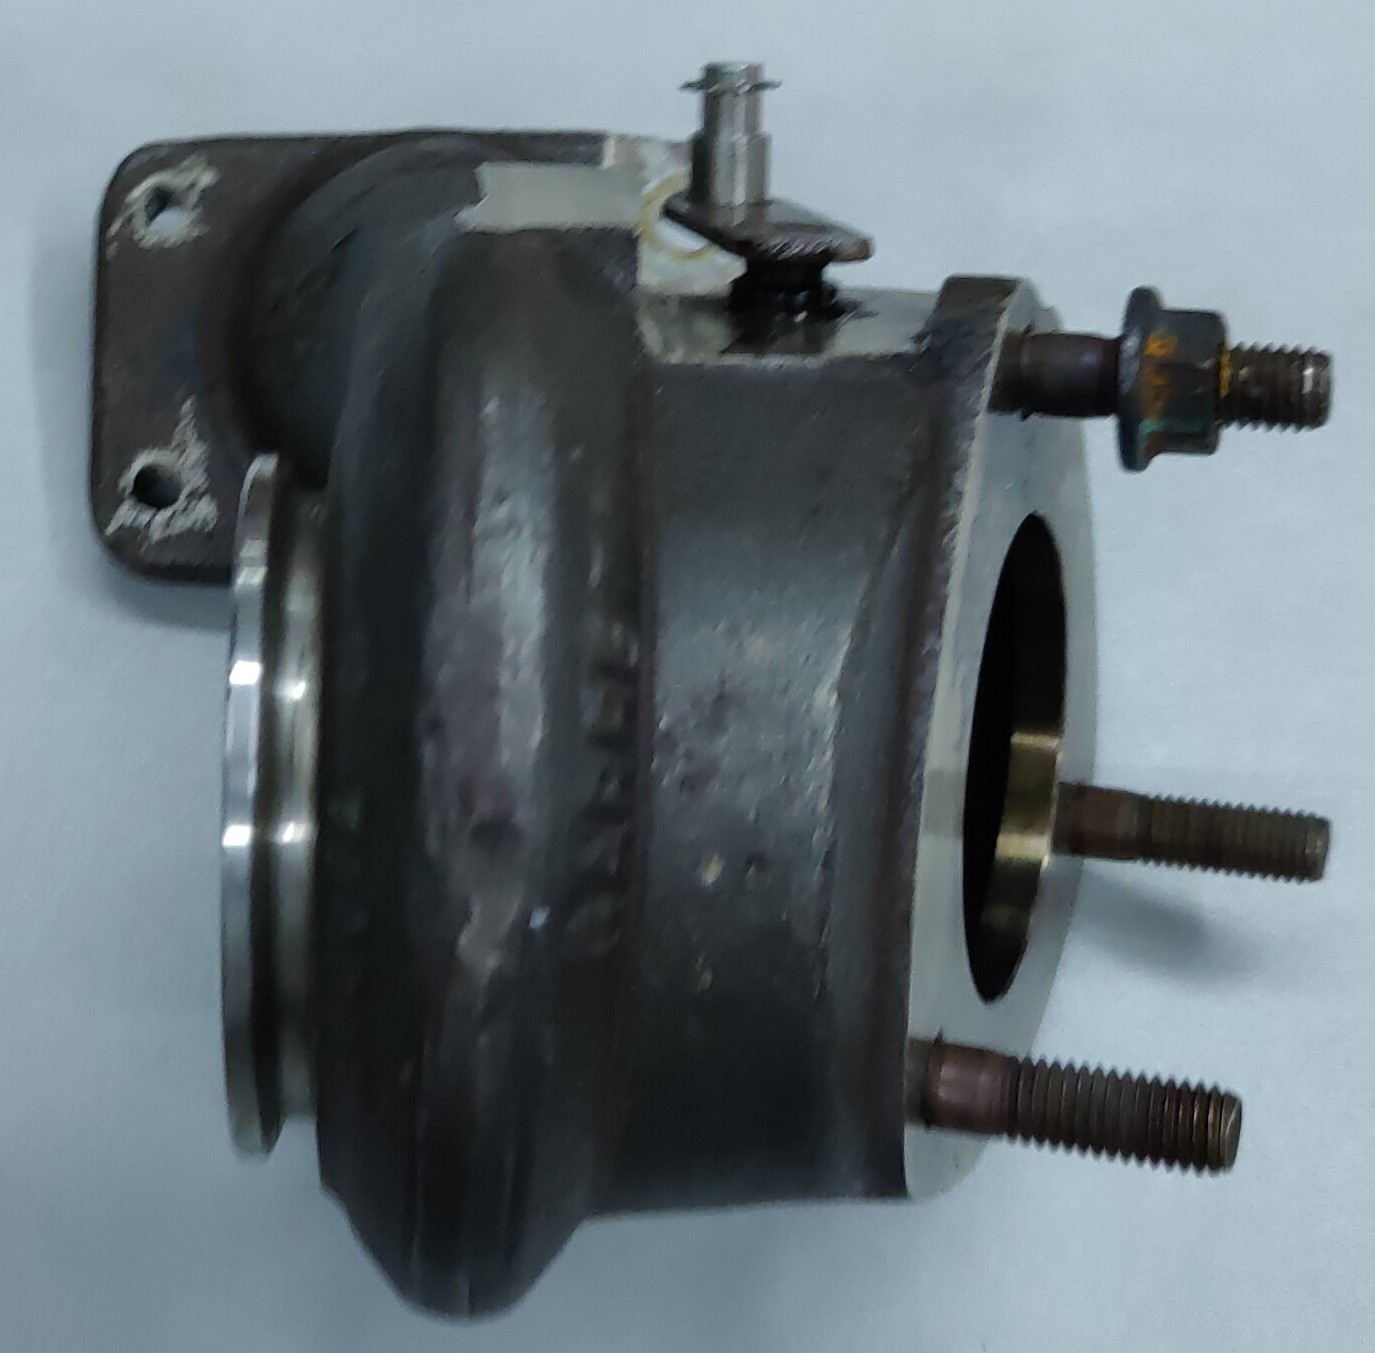
\includegraphics[width=\textwidth]{turbine}
		\caption{涡轮机}
		\label{turbine}
	\end{minipage}
	\begin{minipage}[b]{0.4\textwidth}
		\centering
		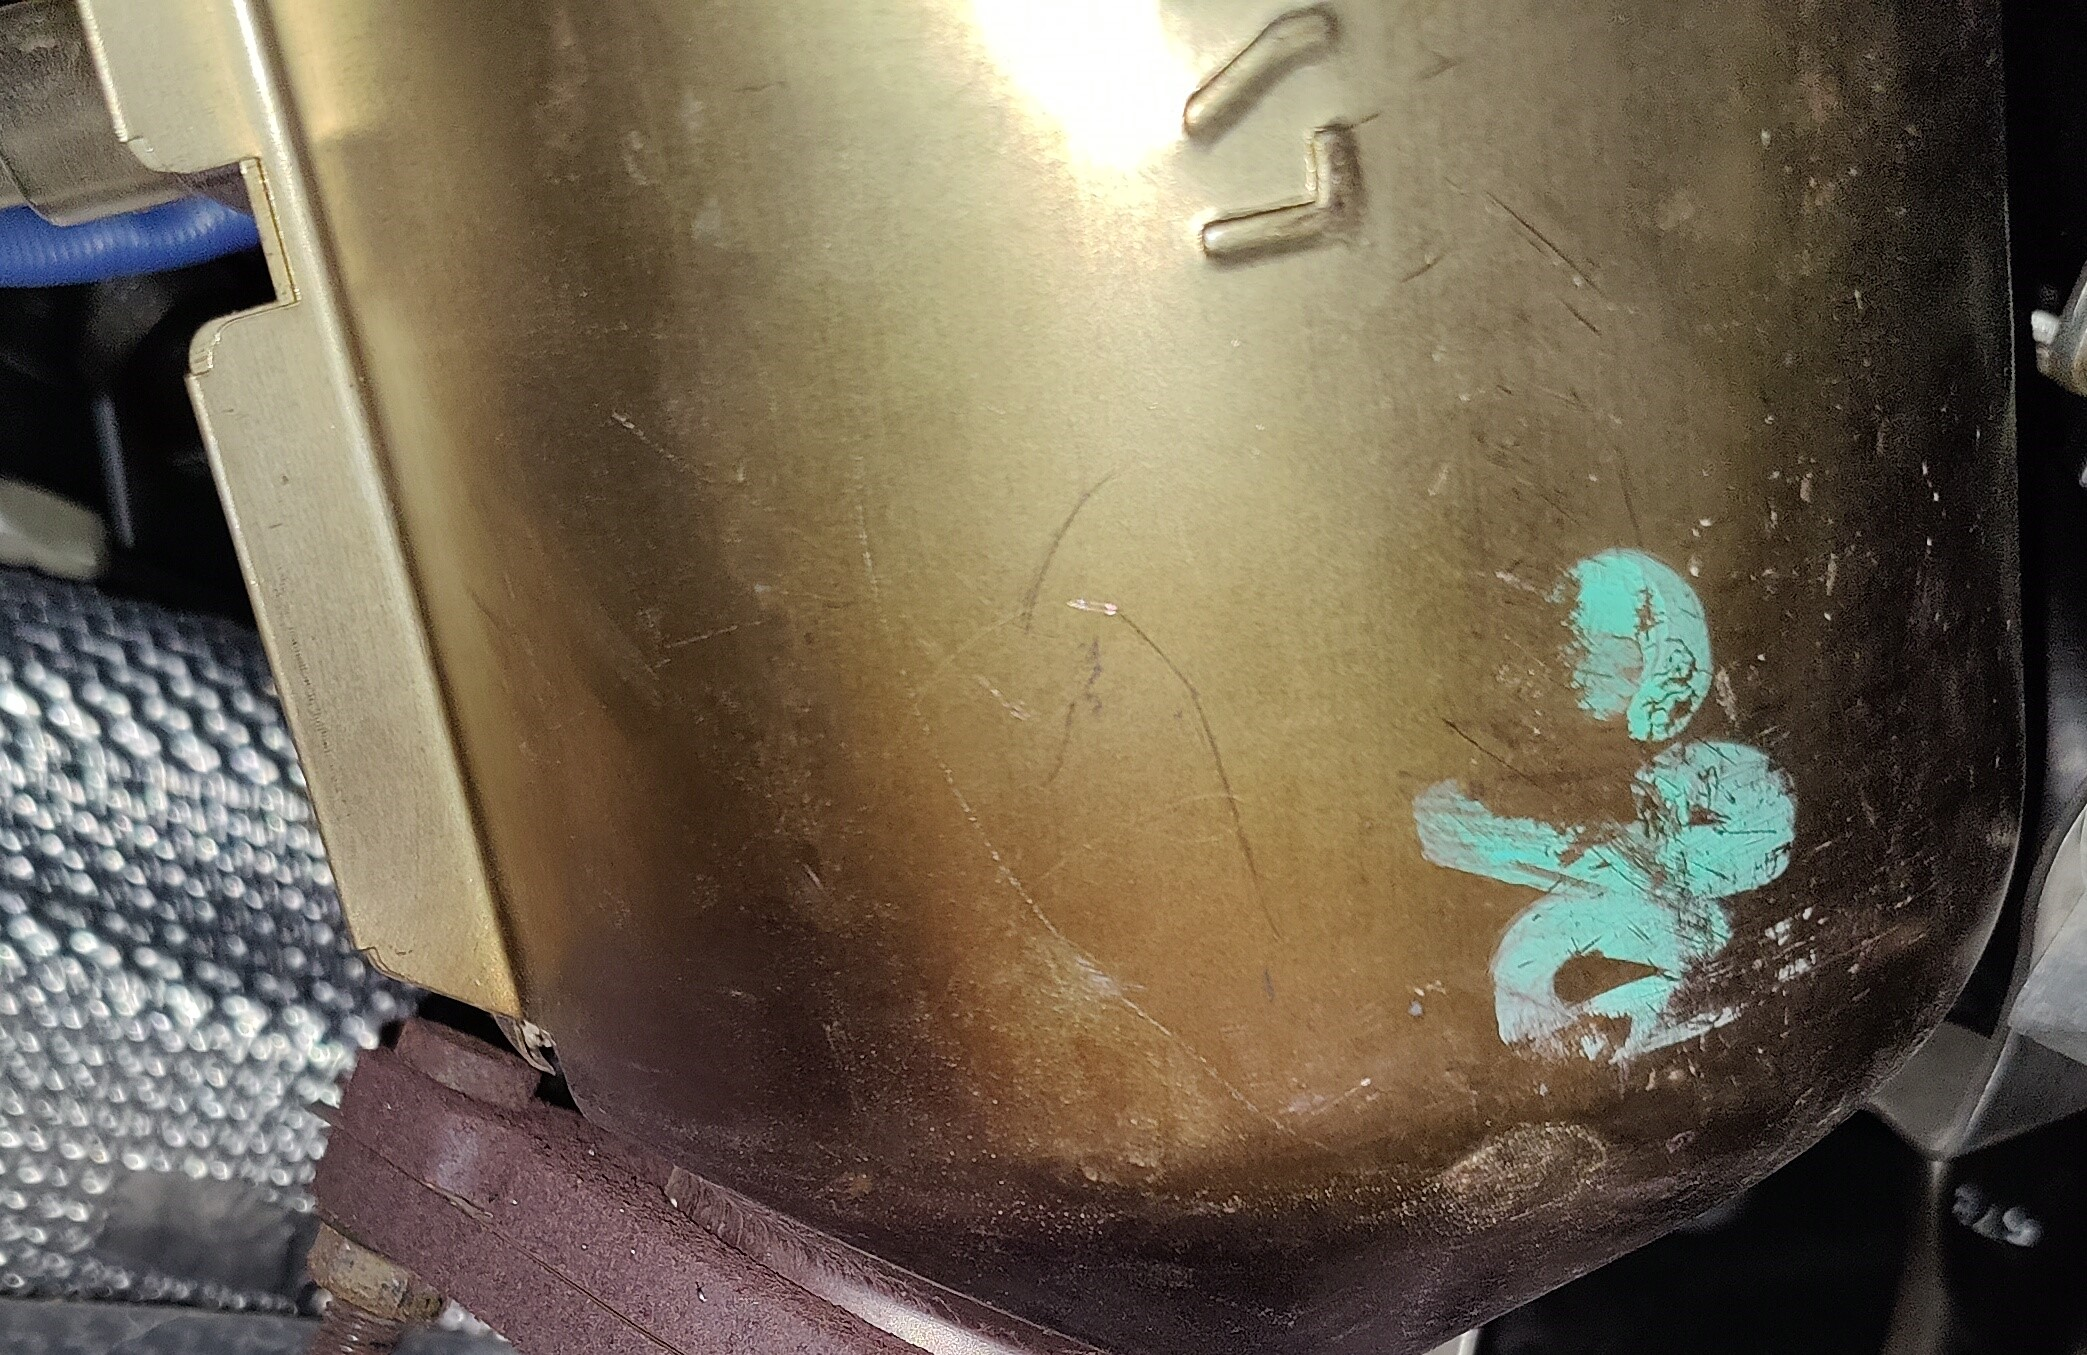
\includegraphics[width=\textwidth]{three-way catalytic converter}
		\caption{三元催化转换器}
		\label{three-way catalytic converter}
	\end{minipage}
	\begin{minipage}[b]{0.25\textwidth}
		\centering
		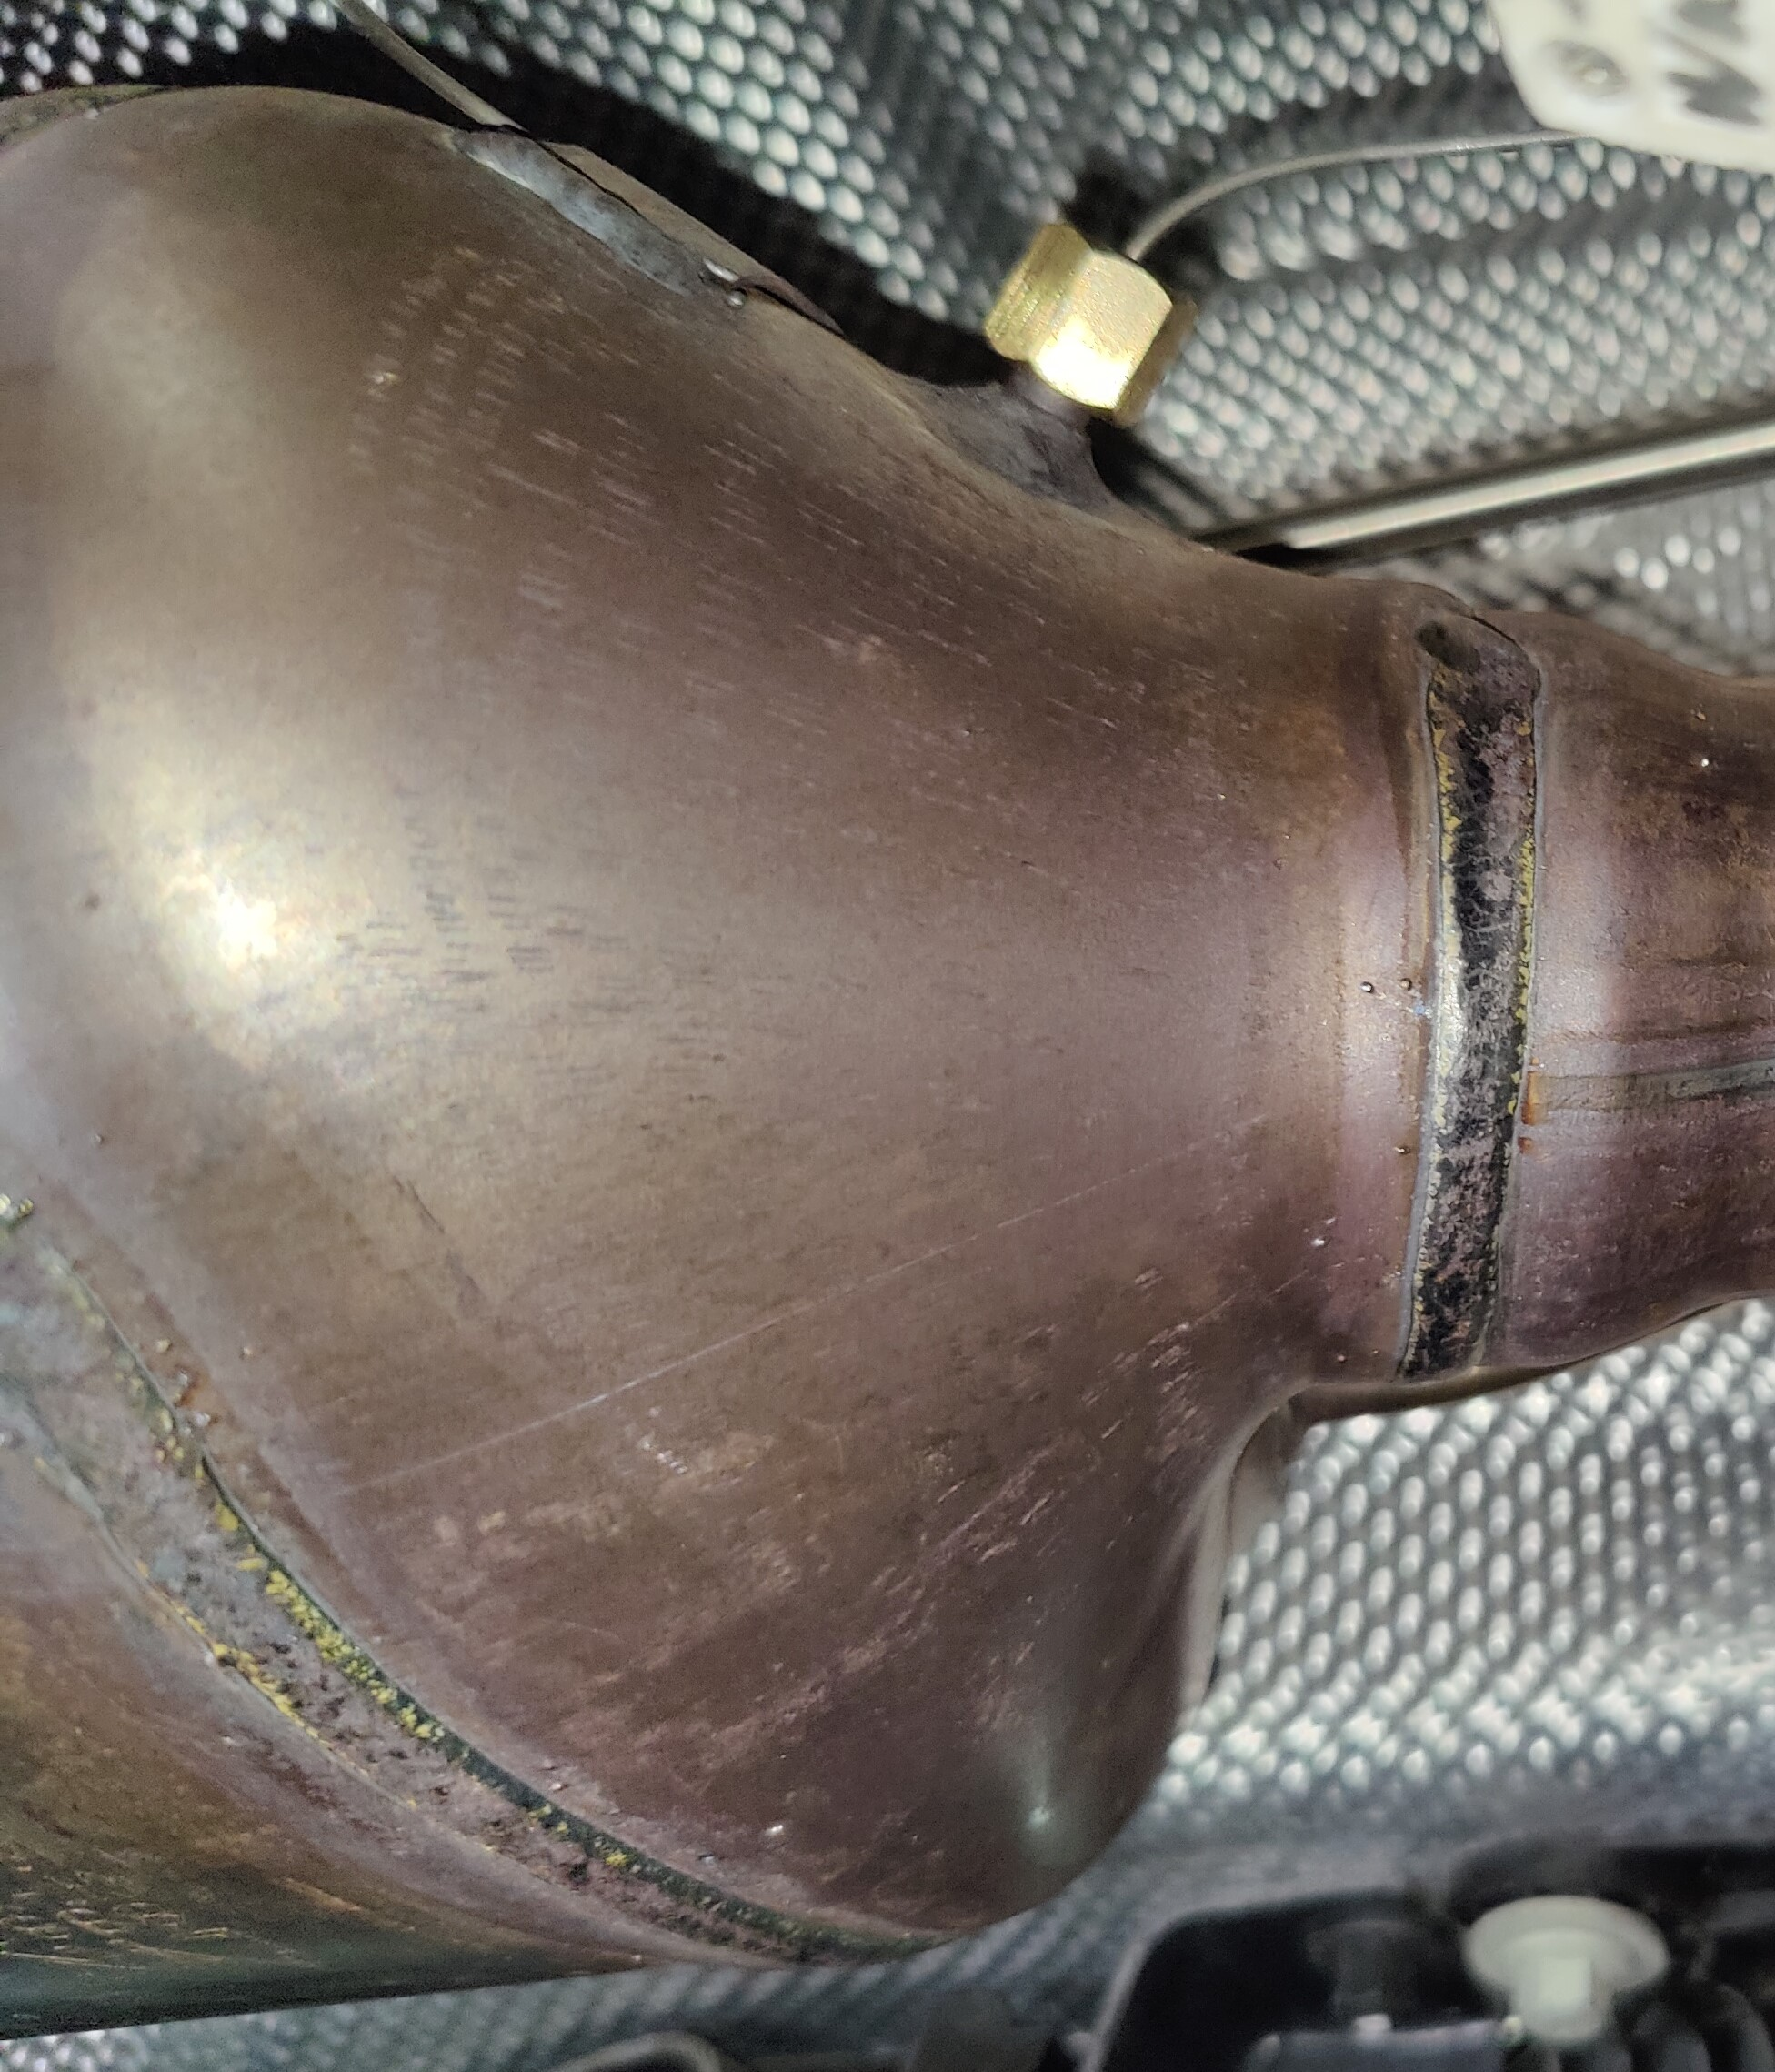
\includegraphics[width=\textwidth]{muffler F}
		\caption{前消声器}
		\label{muffler F}
	\end{minipage}
	\begin{minipage}[b]{0.55\textwidth}
		\centering
		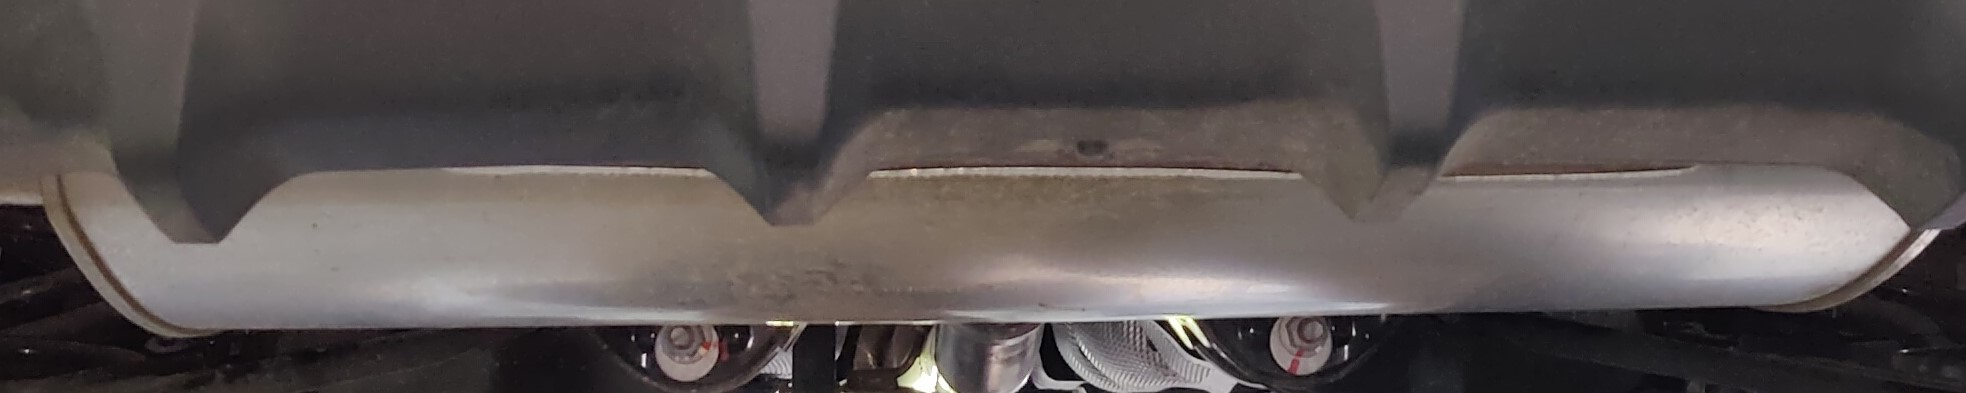
\includegraphics[width=\textwidth]{muffler B}
		\caption{后消声器}
		\label{muffler B}
	\end{minipage}
	\begin{minipage}[b]{0.4\textwidth}
		\centering
		\begin{minipage}[b]{0.45\textwidth}
			\centering
			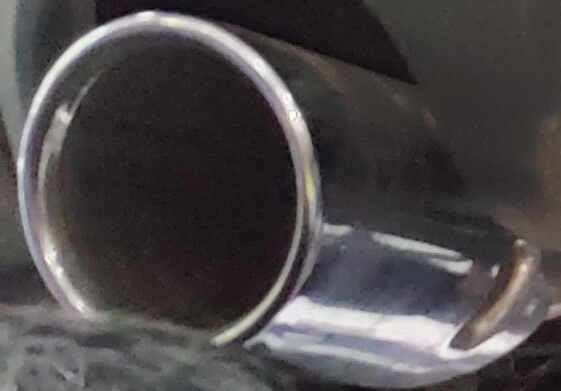
\includegraphics[width=\textwidth]{tail pipe L}
		\end{minipage}
		\begin{minipage}[b]{0.45\textwidth}
			\centering
			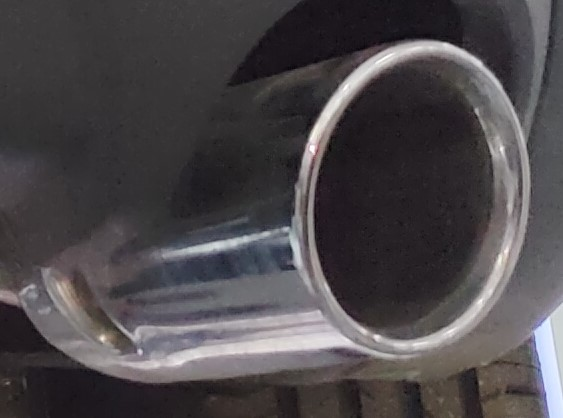
\includegraphics[width=\textwidth]{tail pipe R}
		\end{minipage}
		\caption{排气尾管}
		\label{tail pipe}
	\end{minipage}
\end{figure}

涡轮机是废气涡轮增压器(\cref{exhaust turbocharger})的一个重要组成部分,它的作用是把发动机排出废气的能量转化为机械功来驱动压气机叶轮。本车上使用的径流式涡轮,废气经进气蜗壳由叶轮的径向流入,经轴向流出。涡轮叶片一般在\SI{900}{\celsius}的高温排气冲击下工作,承受巨大的离心力,由镍基耐热合金钢或陶瓷材料制成;蜗壳用耐热合金铸铁铸成,外表面呈黑色,内表面光洁。

由于增压器的热负荷较大,单靠机油不足以满足增压器散热需求,\cref{exhaust turbocharger detached}中间那根较长的软管便是冷却水的管路,与发动机的冷却系统联通。冷却液自增压器中间体上的冷却液进口流入中间体水套,从冷却液出口流回发动机冷却系统。

\cref{exhaust turbocharger detached}所示的涡轮增压系统还带有放气阀(\cref{wastgate valve})。当增压压力达到一阈值后,ECU控制放气阀打开使部分排气不经过涡轮直接排出增压器,防止增压压力和涡轮转速过大造成压气机的阻塞。

\begin{figure}[htbp]
	\centering
	\begin{minipage}[b]{0.4\textwidth}
		\centering
		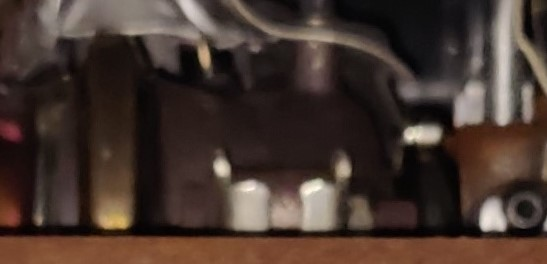
\includegraphics[width=\textwidth]{exhaust turbocharger}
		\caption{废气涡轮增压器}
		\label{exhaust turbocharger}
	\end{minipage}
	\centering
	\begin{minipage}[b]{0.35\textwidth}
		\centering
		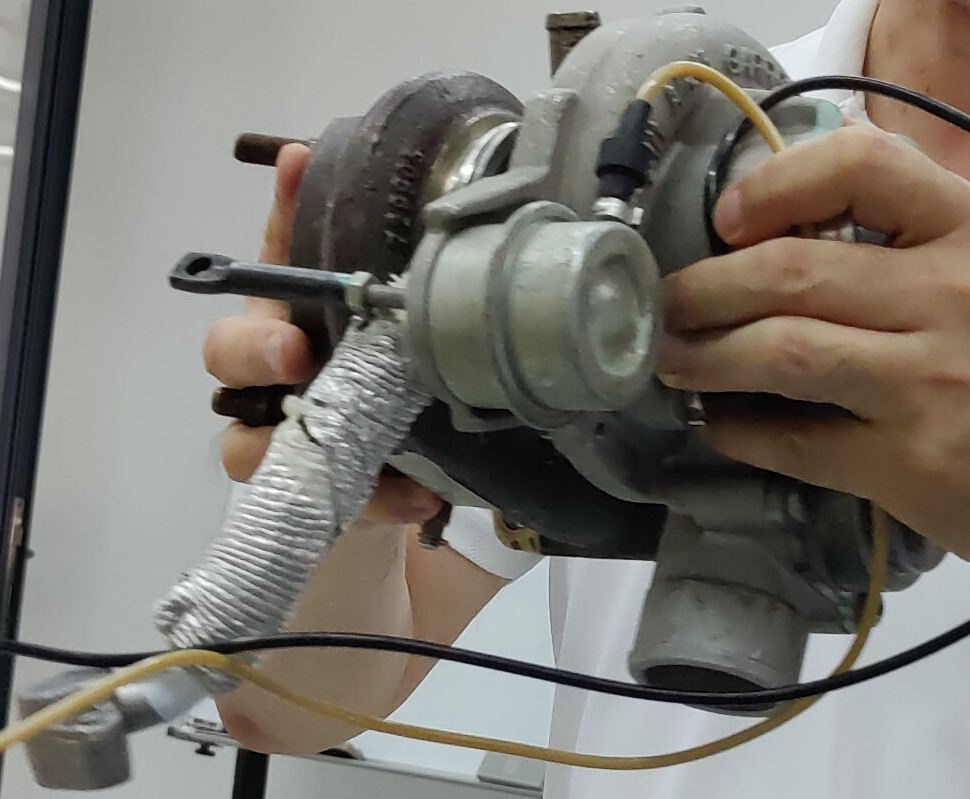
\includegraphics[width=0.8\textwidth]{exhaust turbocharger detached}
		\caption{拆下的废气涡轮增压器}
		\label{exhaust turbocharger detached}
	\end{minipage}
	\begin{minipage}[b]{0.18\textwidth}
		\centering
		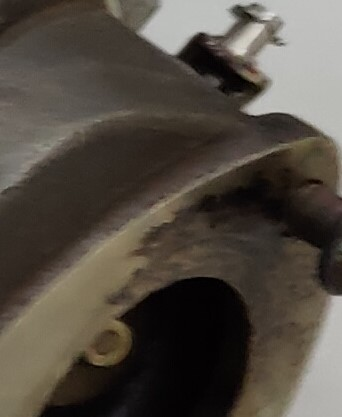
\includegraphics[width=\textwidth]{wastgate valve}
		\caption{放气阀}
		\label{wastgate valve}
	\end{minipage}
\end{figure}

三元催化转换器以排气中的\ce{CO}和\ce{HC}作为还原剂,在把\ce{NO_x}还原成\ce{N2}和\ce{O2}的同时把\ce{CO}和\ce{HC}氧化为\ce{CO2}和\ce{H2O},反应式为
\begin{align}
	\ce{CO + O2 & -> CO2} \nonumber       \\
	\ce{HC + O2 & -> H2O + CO2} \nonumber \\
	\ce{NO_X    & -> N2 + O2} \nonumber
\end{align}
三元催化转换器将带有很多小孔的蜂窝状陶瓷作为载体,表面附着一层薄的氧化铝中间镀层,再在其上镀以由铂、钯、铑等贵金属制成的催化剂。催化转换器外面用金属外壳封闭,并焊在排气管路内,避免被随意拆卸。三元催化转换器要求车辆使用无铅汽油,温度超过\SI{350}{\celsius}时才会工作,最重要的是要求发动机混合气浓度始终在理论空燃比附近。最后这点是通过氧传感器实现的。

三元催化转换器前后各有一个氧传感器,其中前氧传感器起主要作用,后氧传感器的用处主要是检测催化转换器是否工作正常。ECU通过进气量、喷油量及排气中氧浓度可实现过量空气系数$\lambda$的闭环控制。氧传感器的传感元件一般是在陶瓷管基体上附着有\ce{ZrO2}涂层,外侧通排气,内侧通大气。当陶瓷管温度在\SI{350}{\celsius}左右时具有固态电解质的特性。如\cref{voltage response curve},当混合气偏浓时,排气中\ce{O2}浓度低,陶瓷管内外\ce{O^2-}浓度差较高,氧传感器输出电压高(约\SI{900}{\mV});反之当混合气偏稀时输出电压较低(约\SI{100}{\mV})。氧传感器输出电压在理论空燃比附近对过量空气系数的变化很敏感,ECU据此不断修正喷油量使得$\lambda$始终在最佳范围内。

由于缸内直喷易产生碳烟,排气系统上设置有颗粒捕集器以满足排放法规要求。

\begin{figure}[htbp]
	\centering
	\begin{minipage}[b]{0.45\textwidth}
		\centering
		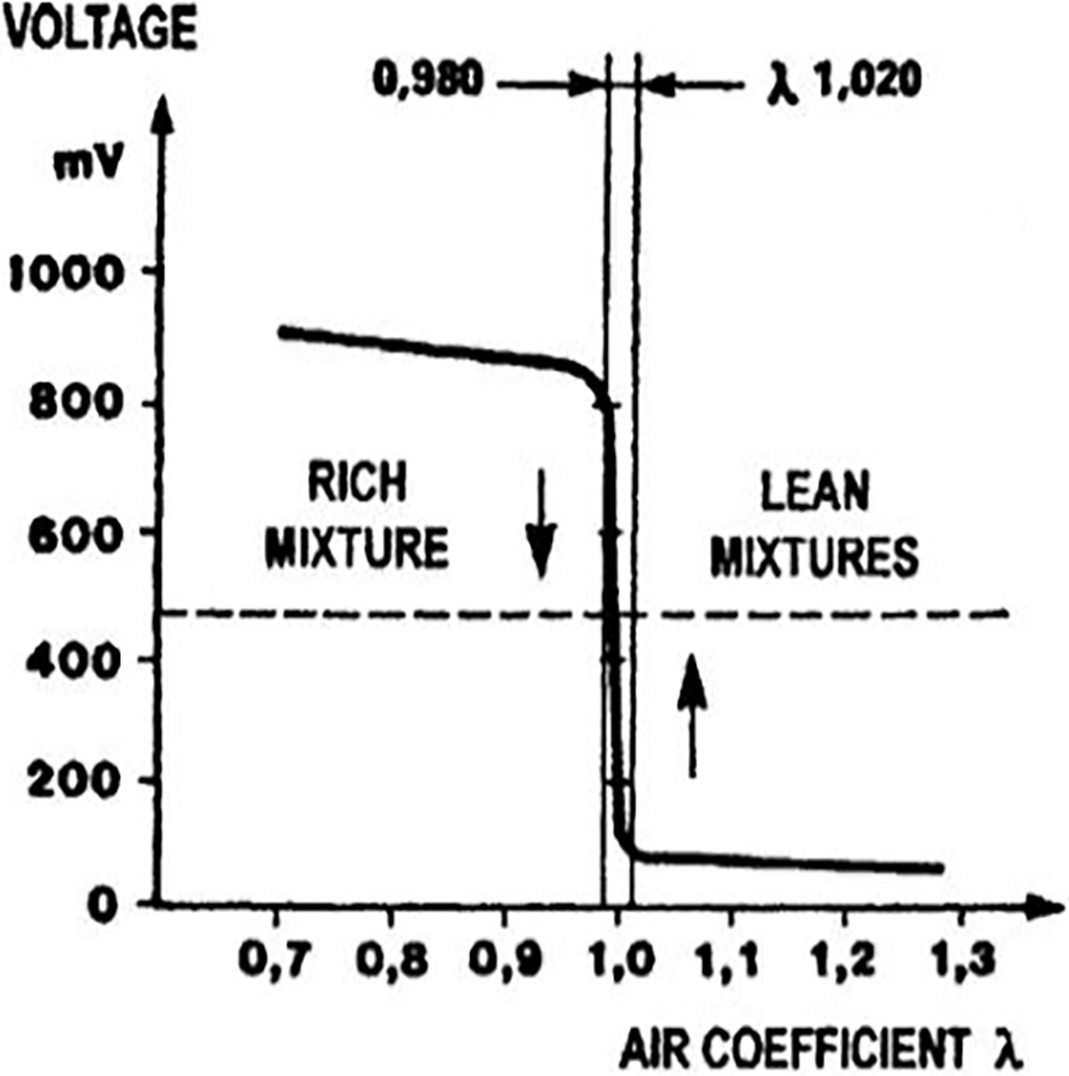
\includegraphics[width=\textwidth]{voltage response curve}
		\caption{氧传感器的电压曲线}
		\label{voltage response curve}
	\end{minipage}
\end{figure}

消声器的主要功能是减小排气的噪声。由于发动机为间歇排气,在排气管中会引起压力的脉动,排气的温度、压力、速度等也很高,具有一定能量。消声器的通过吸收、扩张、共振、干涉等方式耗散排气中的能量,达到消声的目的。一个消声器中常有不同形式的多个腔组合(\cref{muffler dissect}),以提高消声效果。

\begin{figure}[htbp]
	\centering
	\begin{minipage}[b]{0.6\textwidth}
		\centering
		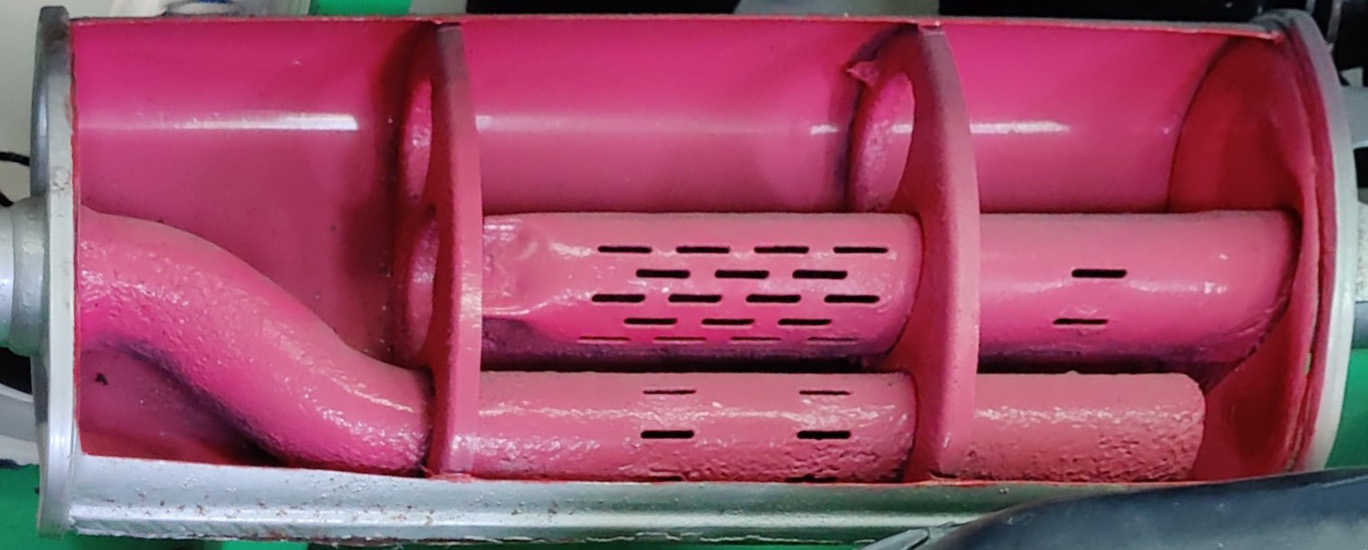
\includegraphics[width=\textwidth]{muffler dissect}
		\caption{剖开的排气消声器}
		\label{muffler dissect}
	\end{minipage}
\end{figure}

\subsection{请简述汽车动力总成如何固定在车身上。}

发动机和变速箱刚性连接构成汽车动力总成,但动力总成与车身的连接是柔性的,这需要通过悬置来实现。悬置的功用主要有支撑、限位和隔振。支撑指悬置必须能承受动力总成的质量,使其不至于产生过大的静位移;限位指动力总成在受到各种干扰力作用的情况下,悬置应能有效的限制其最大位移以避免干涉;隔振指悬置一方面要阻止作为振源的发动机向车身传递振动,另一方面还要能缓和路面不平激励等传给发动机的振动和冲击。

从隔振角度来说,希望悬置较软,以期将振动更好地隔离;而从支承和限位角度来说,为使发动机舱能布置紧凑,又希望悬置越硬越好。在悬置设计中如何最优化选取悬置刚度是一个极为重要的问题。同时,为了使振动得到迅速衰减,发动机悬置还应具有适当的的阻尼。

领克02车型的动力总成采用三点固定的方式,通过一个后悬置和两个前悬置将动力总成与车身连接,如\cref{mount}。\cref{mount B}看得较清楚,我们可以看到,后悬置与发动机和车身的两个连接轴线互相垂直,且两连接处都有橡胶减震块,能有效衰减动力总成相对车身俯仰和偏航两个方向的相对运动,而对侧倾的衰减主要由前面两悬置实现。

当然,这种软连接的形式会对发动机的动力输出造成一定影响,因为部分扭矩被用于克服减震块的阻力。在一些超跑和方程式赛车中有将发动机直接固定在单体壳上的方式,以期最大化动力输出,但会恶化车辆的NVH (Noise, vibration, and harshness) 特性,在乘用车上一般都是用三点式或四点式的悬置将汽车动力总成固定在车身上。

\begin{figure}[htbp]
	\centering
	\subfigure[后悬置]{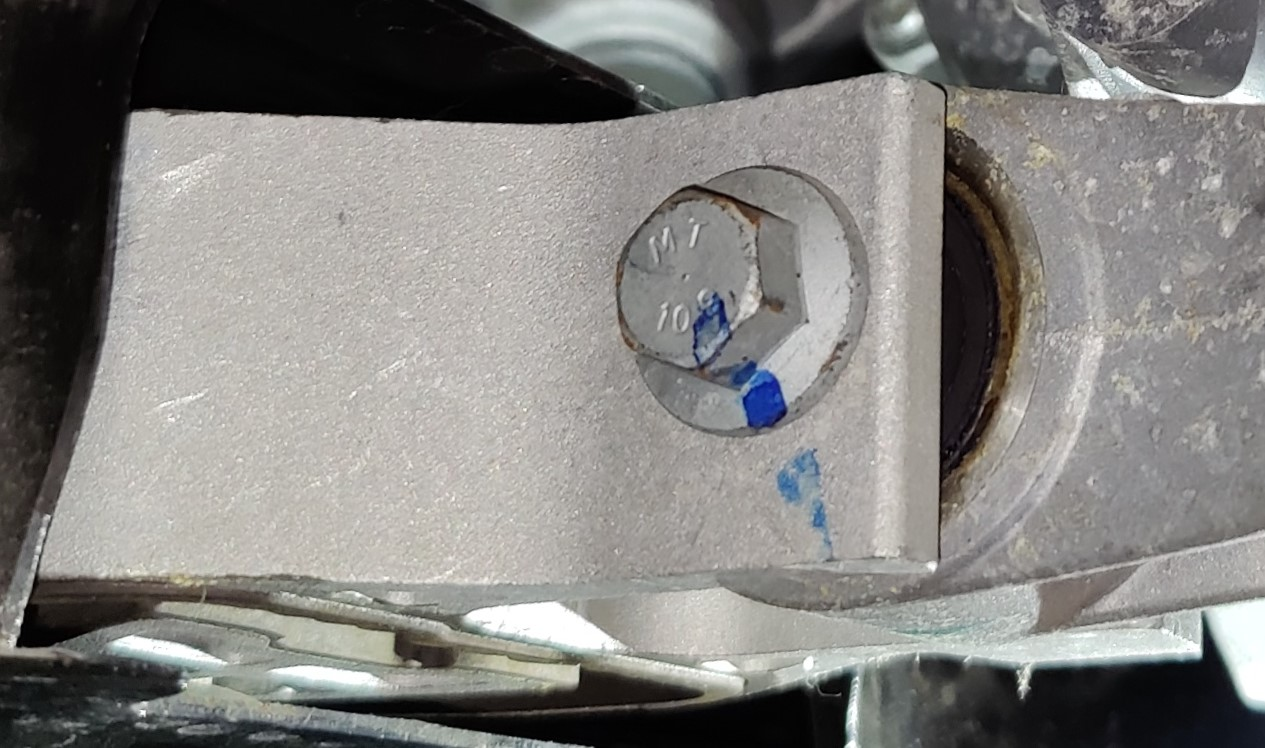
\includegraphics[width=0.6\textwidth]{mount B}\label{mount B}}
	\subfigure[右前悬置]{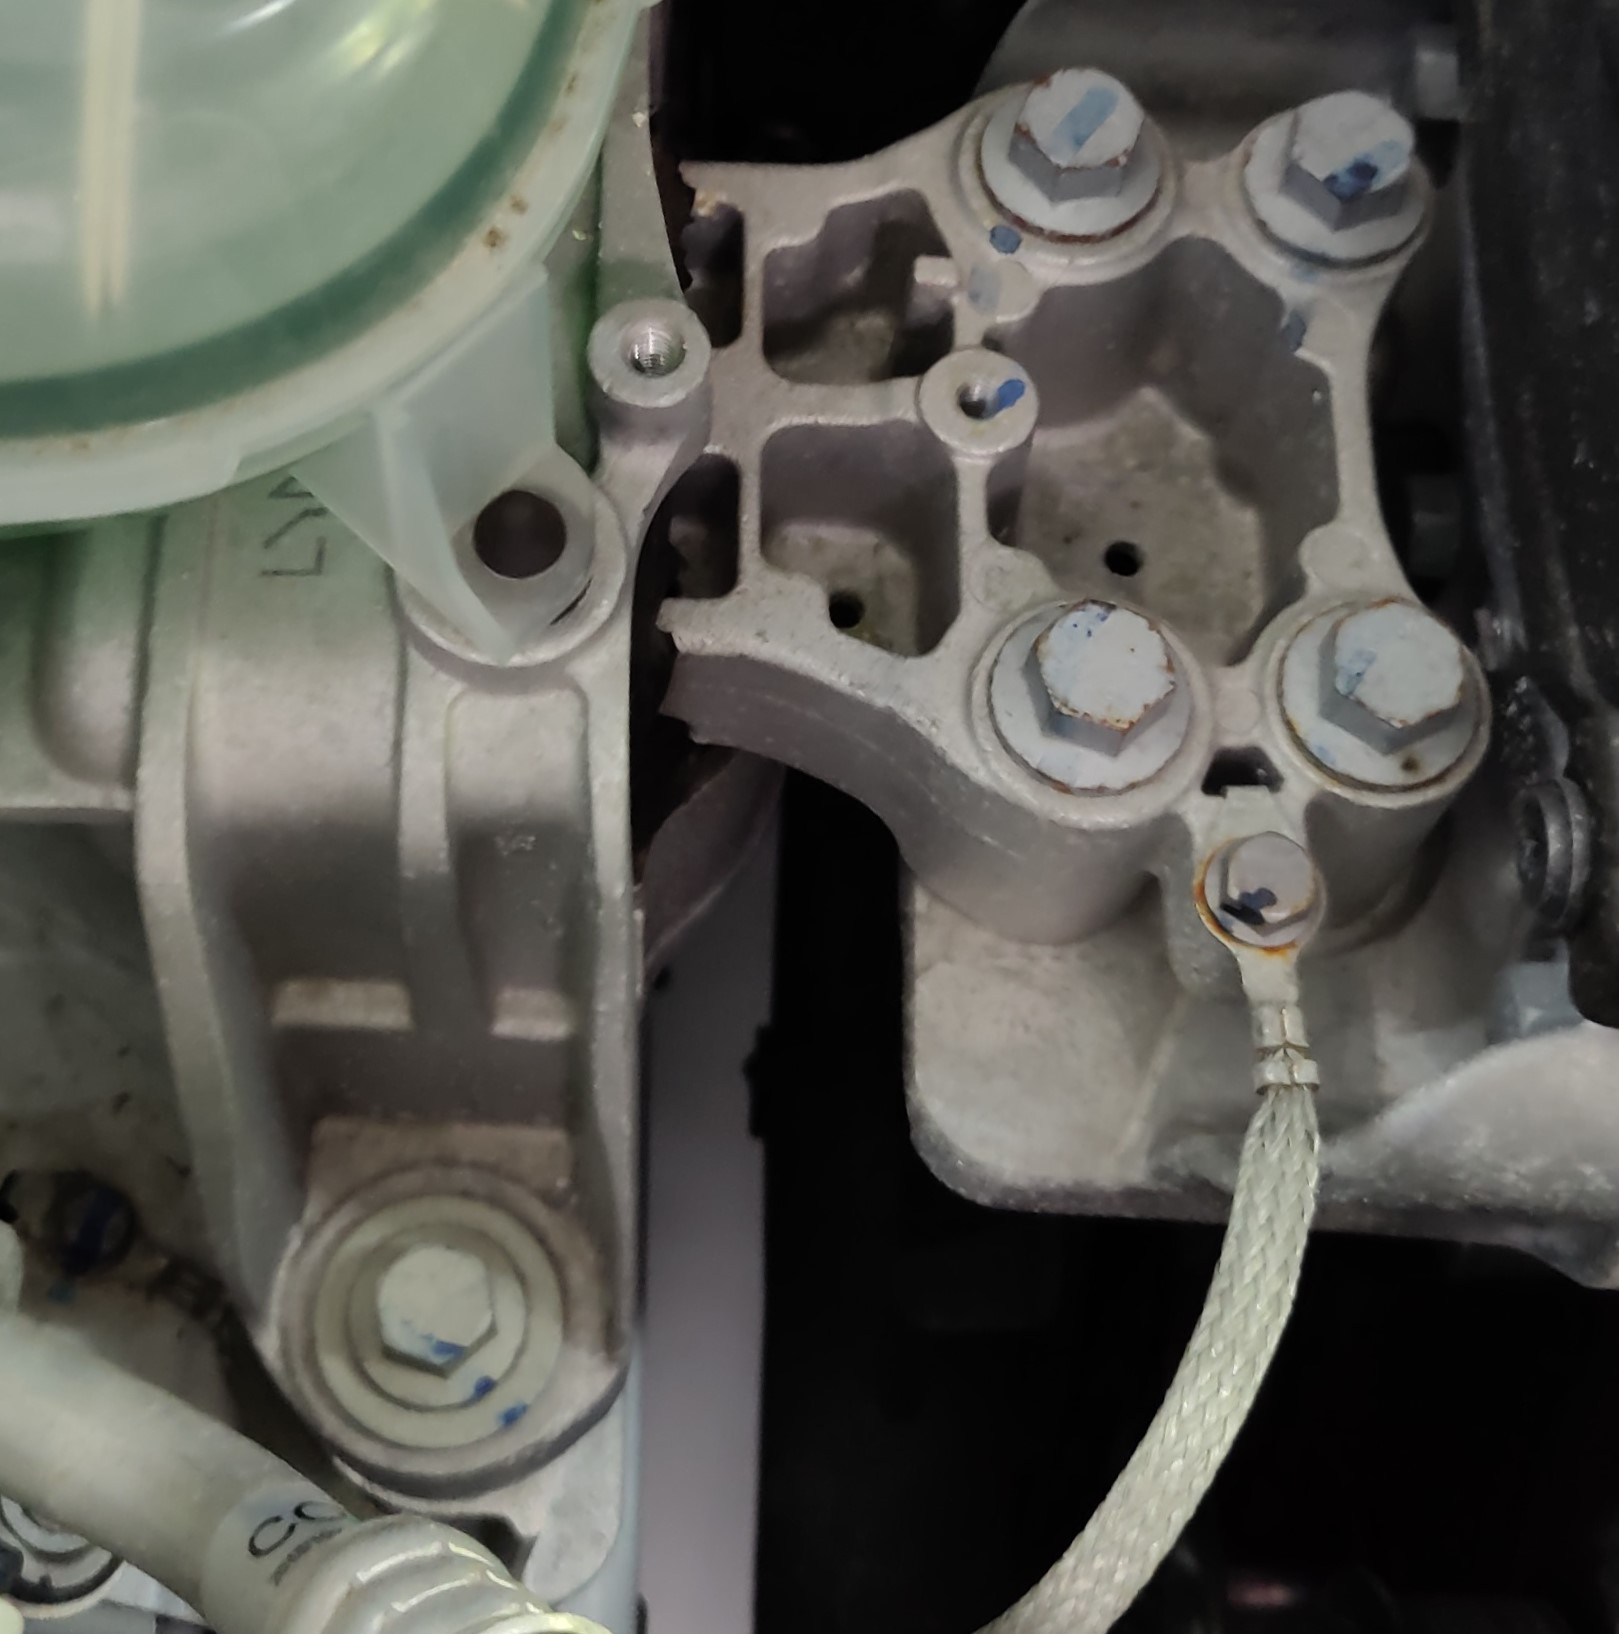
\includegraphics[width=0.4\textwidth]{mount RF}\label{mount RF}}
	\subfigure[左前悬置]{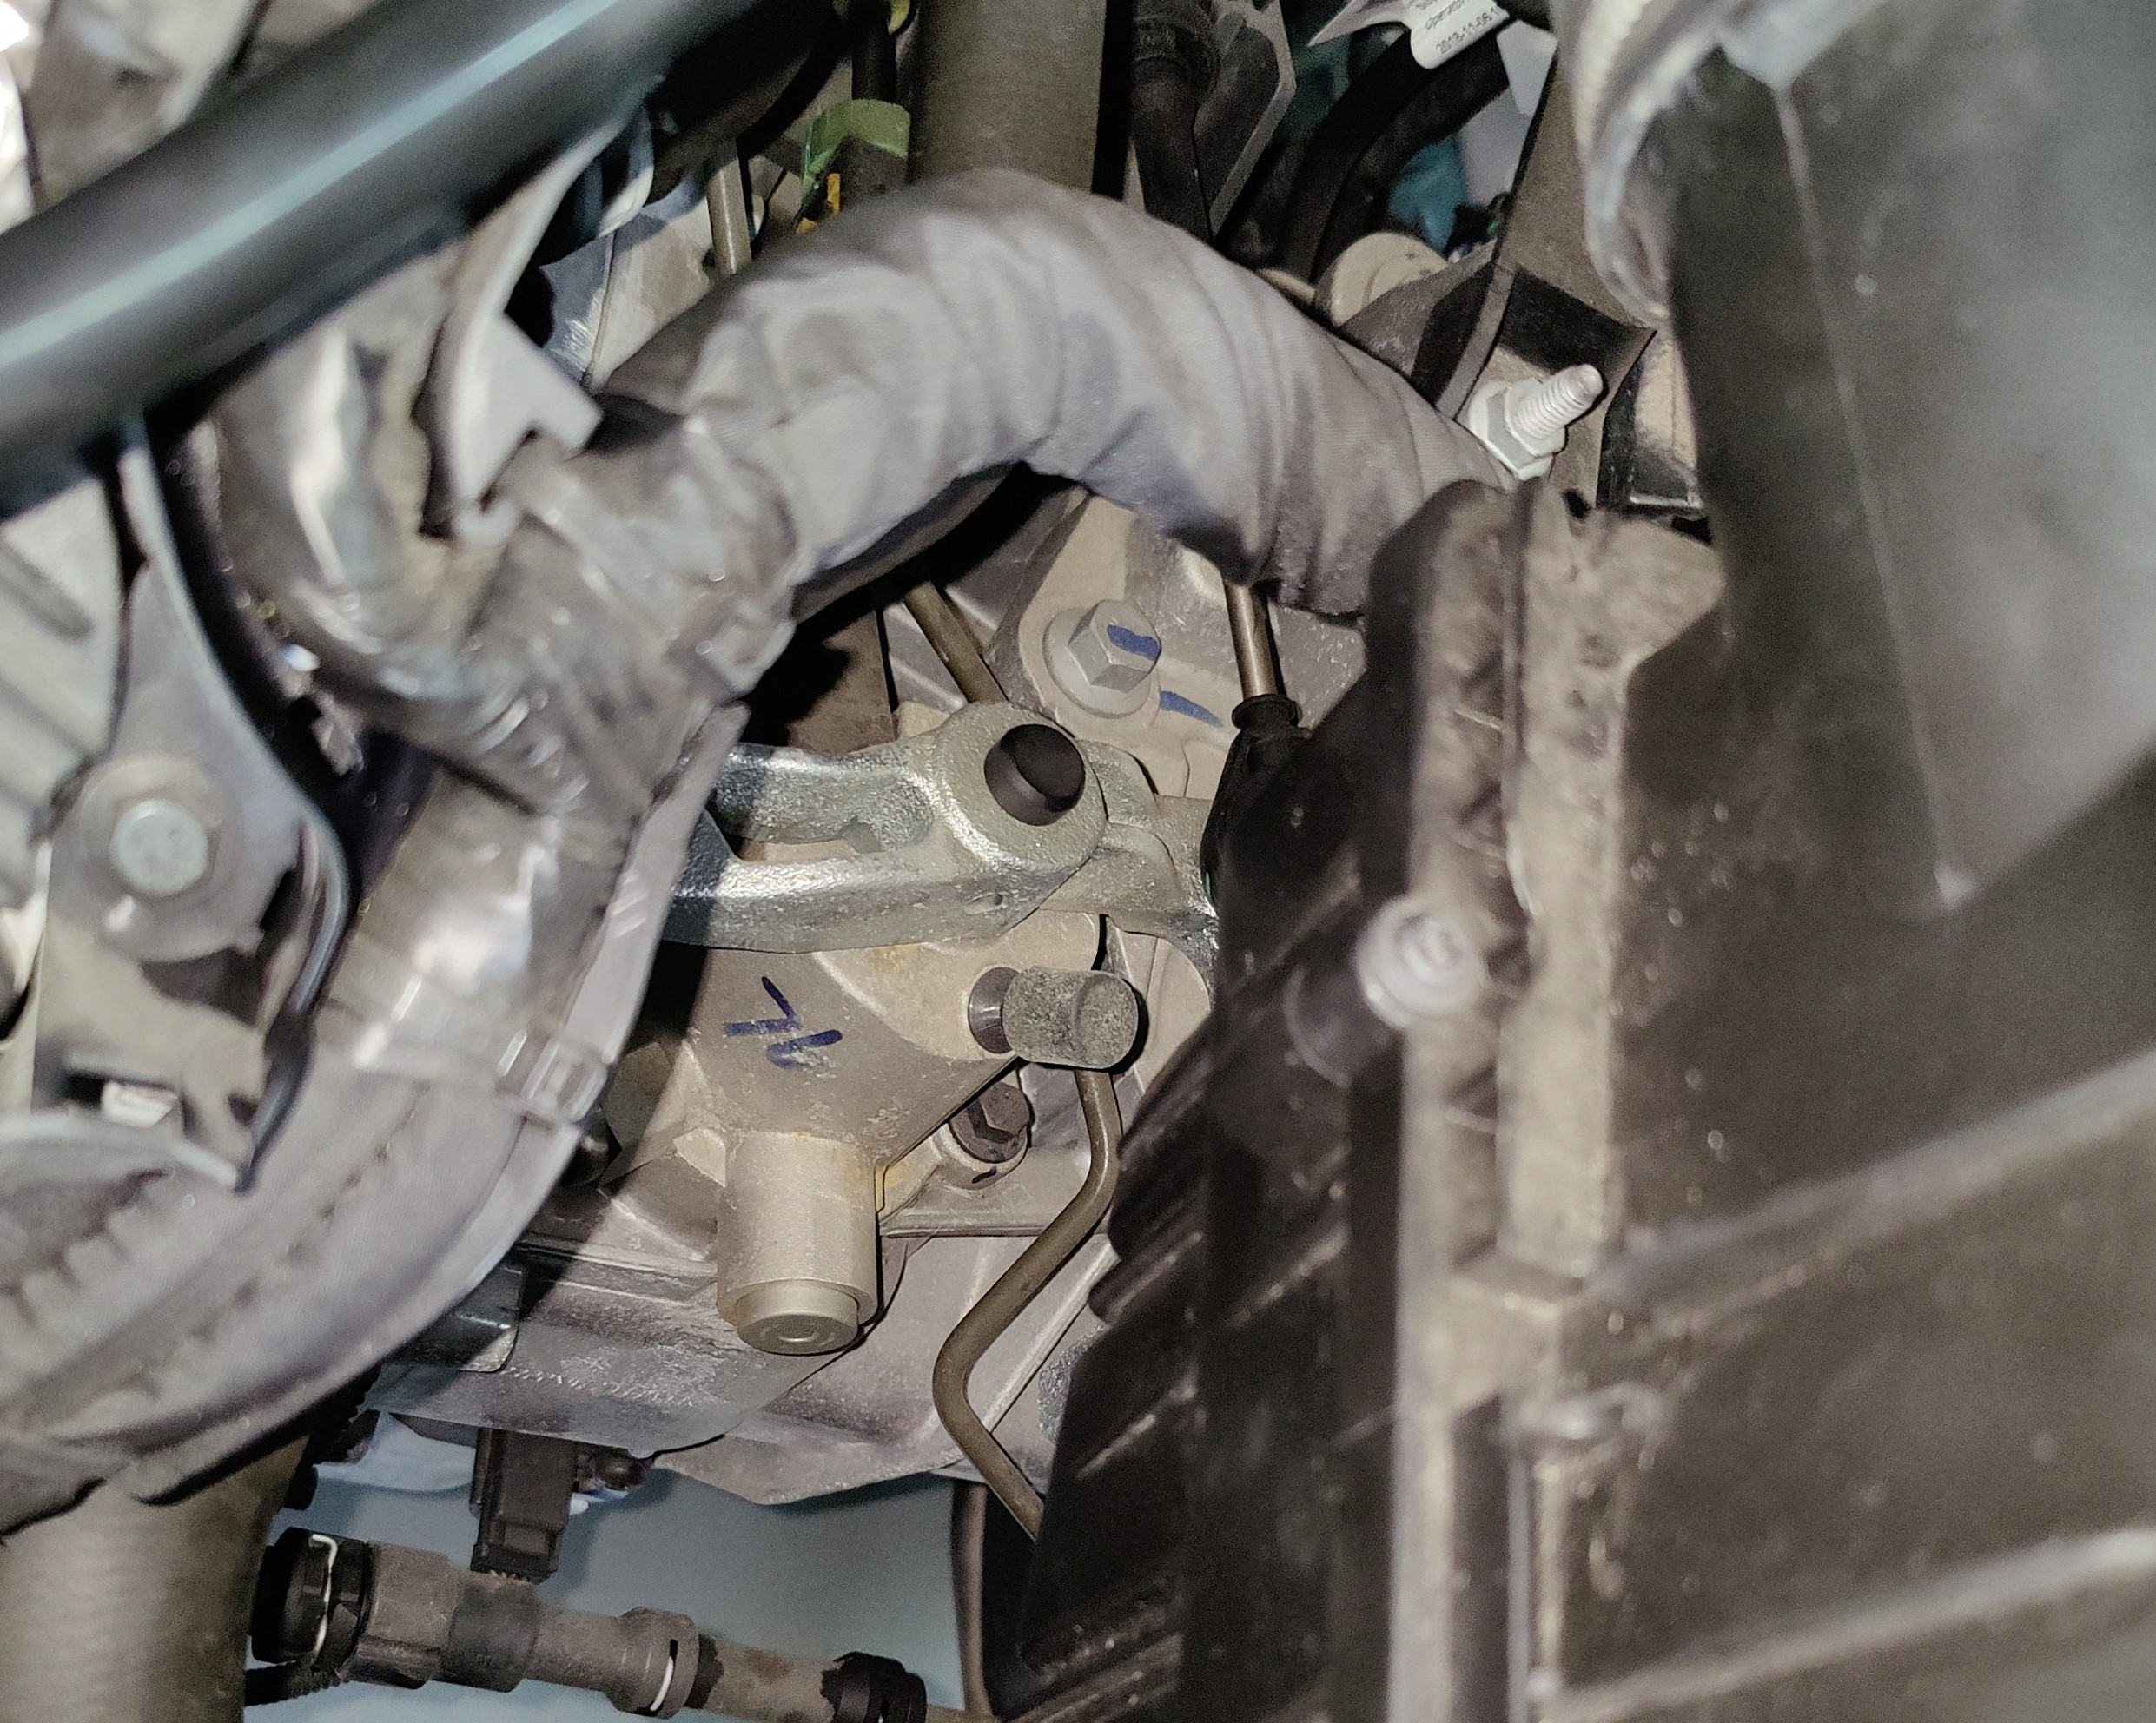
\includegraphics[width=0.5\textwidth]{mount LF}\label{mount LF}}
	\caption{悬置}
	\label{mount}
\end{figure}

\subsection{请简述发动机的控制系统中的传感器和执行器主要有哪些?}

发动机控制系统中的传感器主要有空气流量计、曲轴位置传感器、氧传感器、节气门位置传感器、冷却液温度传感器、爆震传感器、离合器开关;执行器主要有燃油泵继电器、燃油泵、喷油器、点火线圈、凸轮轴调节阀、节气门电机(\cref{sensors and actuators})。

\begin{figure}[htbp]
	\centering
	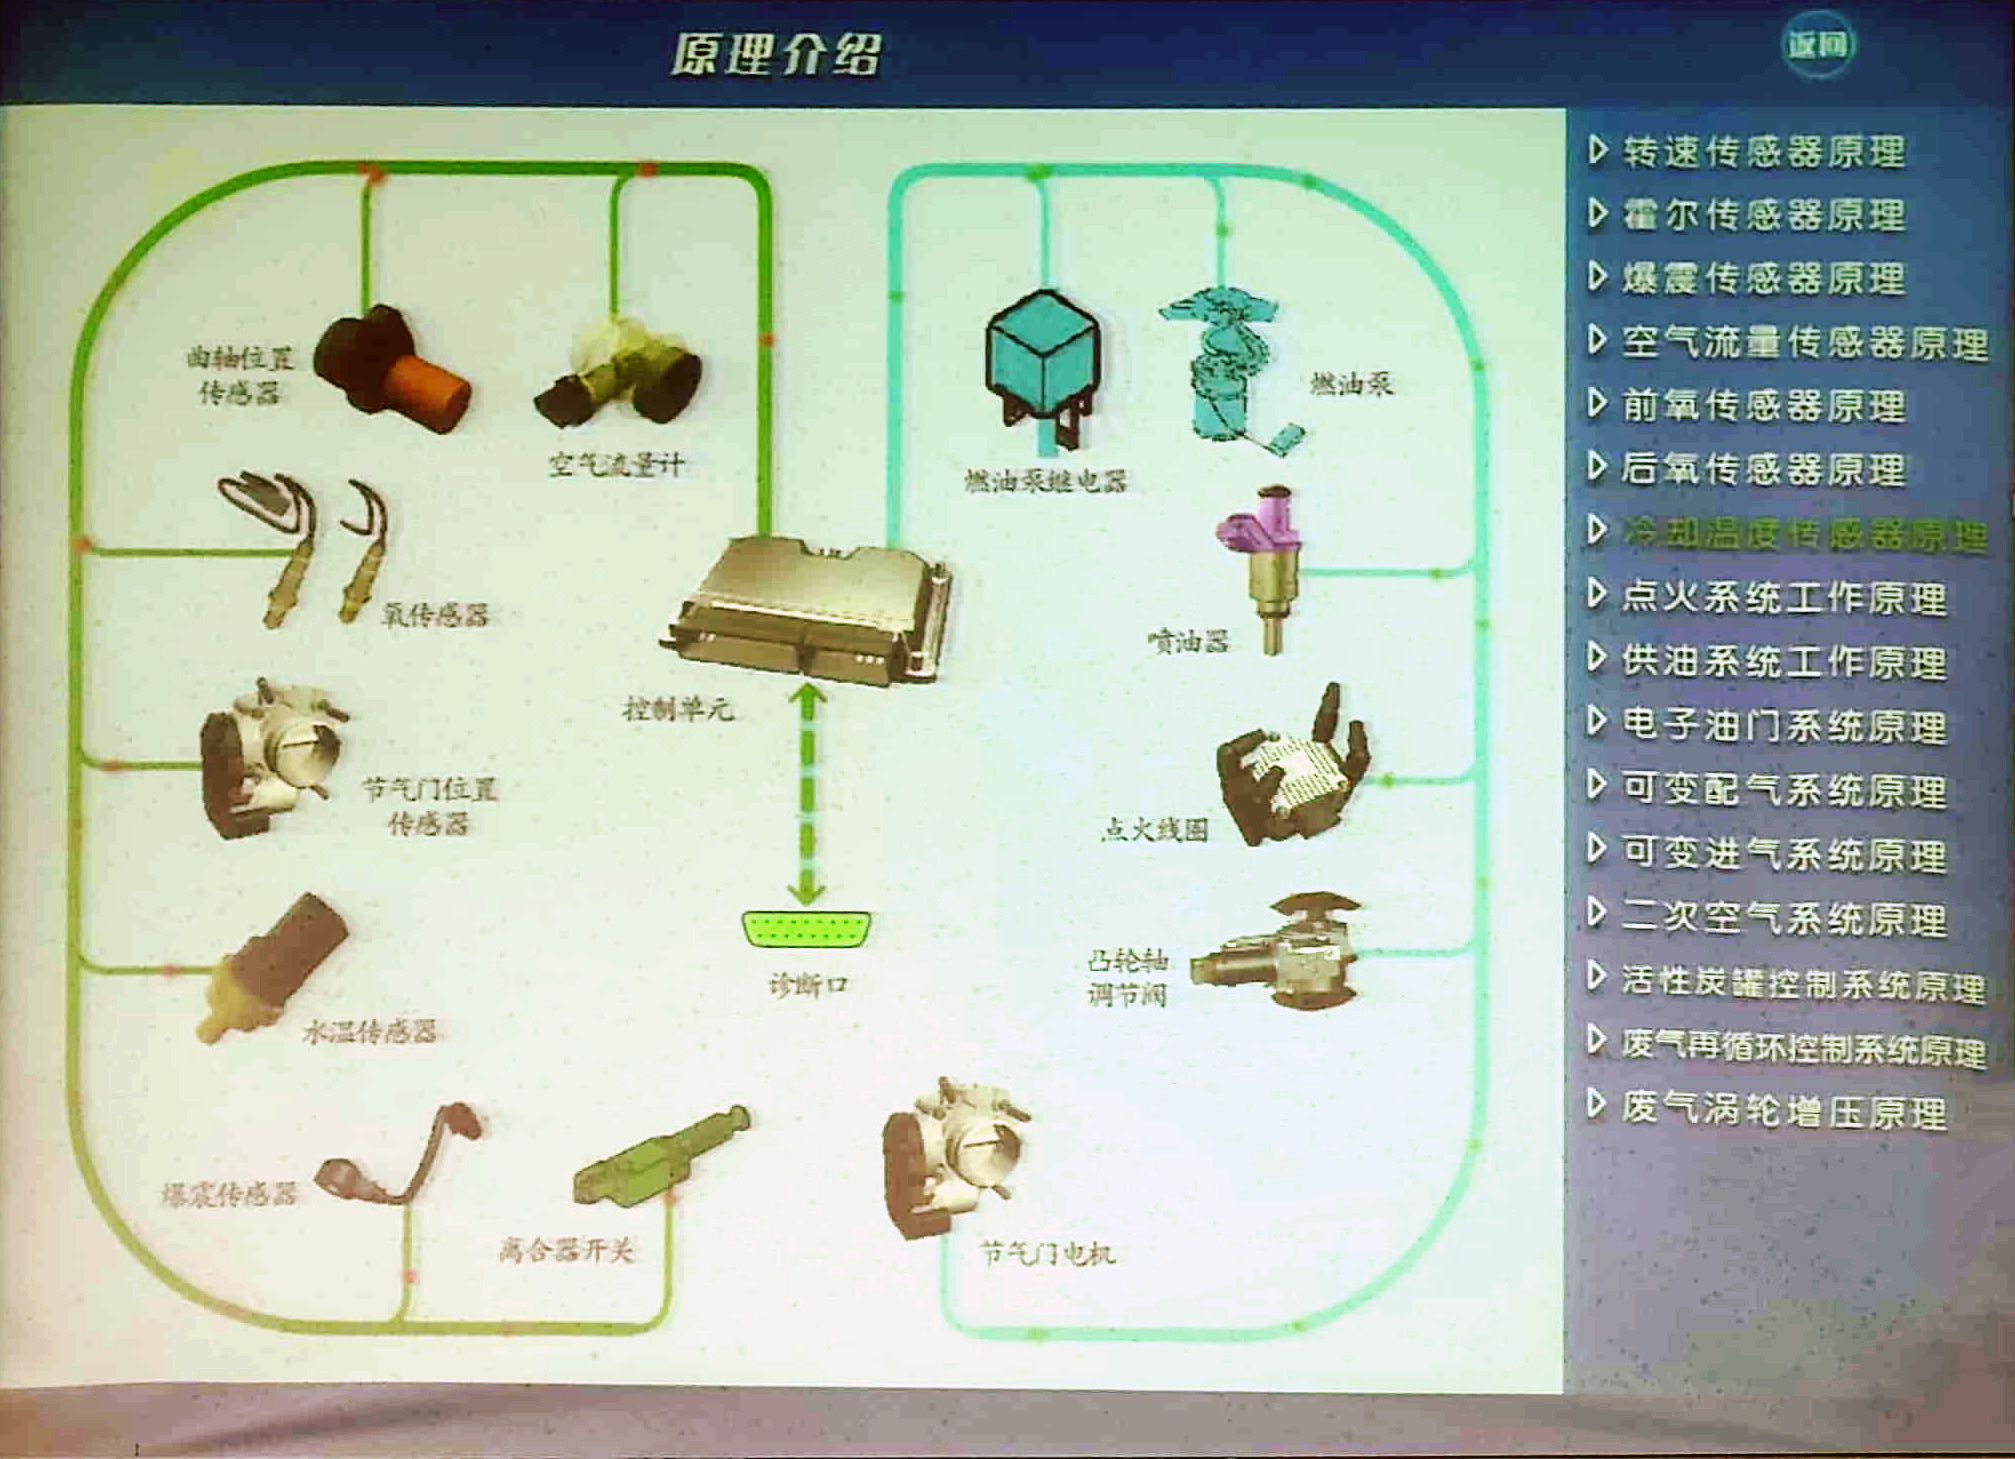
\includegraphics[width=0.9\textwidth]{sensors and actuators}
	\caption{发动机的控制系统中的传感器和执行器}
	\label{sensors and actuators}
\end{figure}

\cref{sensors}所示为发动机控制系统中的部分传感器。现在车用的空气流量计多能直接测得空气的质量流量,分为热线式和热膜式两种,ECU根据空气供给的多少确定喷油量,保证空燃比在理论空燃比附近。曲轴位置传感器有磁电式、光电式和霍尔式等,与安装在曲轴上的靶轮共同工作,主要用于用检测发动机转速,并在凸轮轴相位传感器的配合下确定各缸压缩上止点。前氧传感器和后氧传感器结构类似,都能将排气中氧浓度和空气氧浓度的差转化为输出电压供ECU实现$\lambda$闭环控制。节气门位置传感器是电子节气门系统的一部分,让ECU能闭环控制节气门位置。冷却液温度传感器装在发动机冷却液的出水口上,用来检测出水温度,这个温度一般控制在\SI{90}{\celsius}左右,过高或过低对发动机的工作都是不利的。冷却液温度可通过节温器进行反馈调节,当温度较低时只让冷却液在小回路中循环,便于发动机快速升温;温度高时开启大回路,给发动机较快降温。爆震传感器安装在发动机机体上,它的固有频率设计为与爆震发生时机体的震动频率相近。当发生爆震时,发动机机体与传感器发生共振,传感器输出最大电压信号,表示爆震发生,ECU据此推迟点火,即减小点火提前角,这能有效抑制发动机爆燃。

\begin{figure}[htbp]
	\centering
	\subfigure[空气流量计]{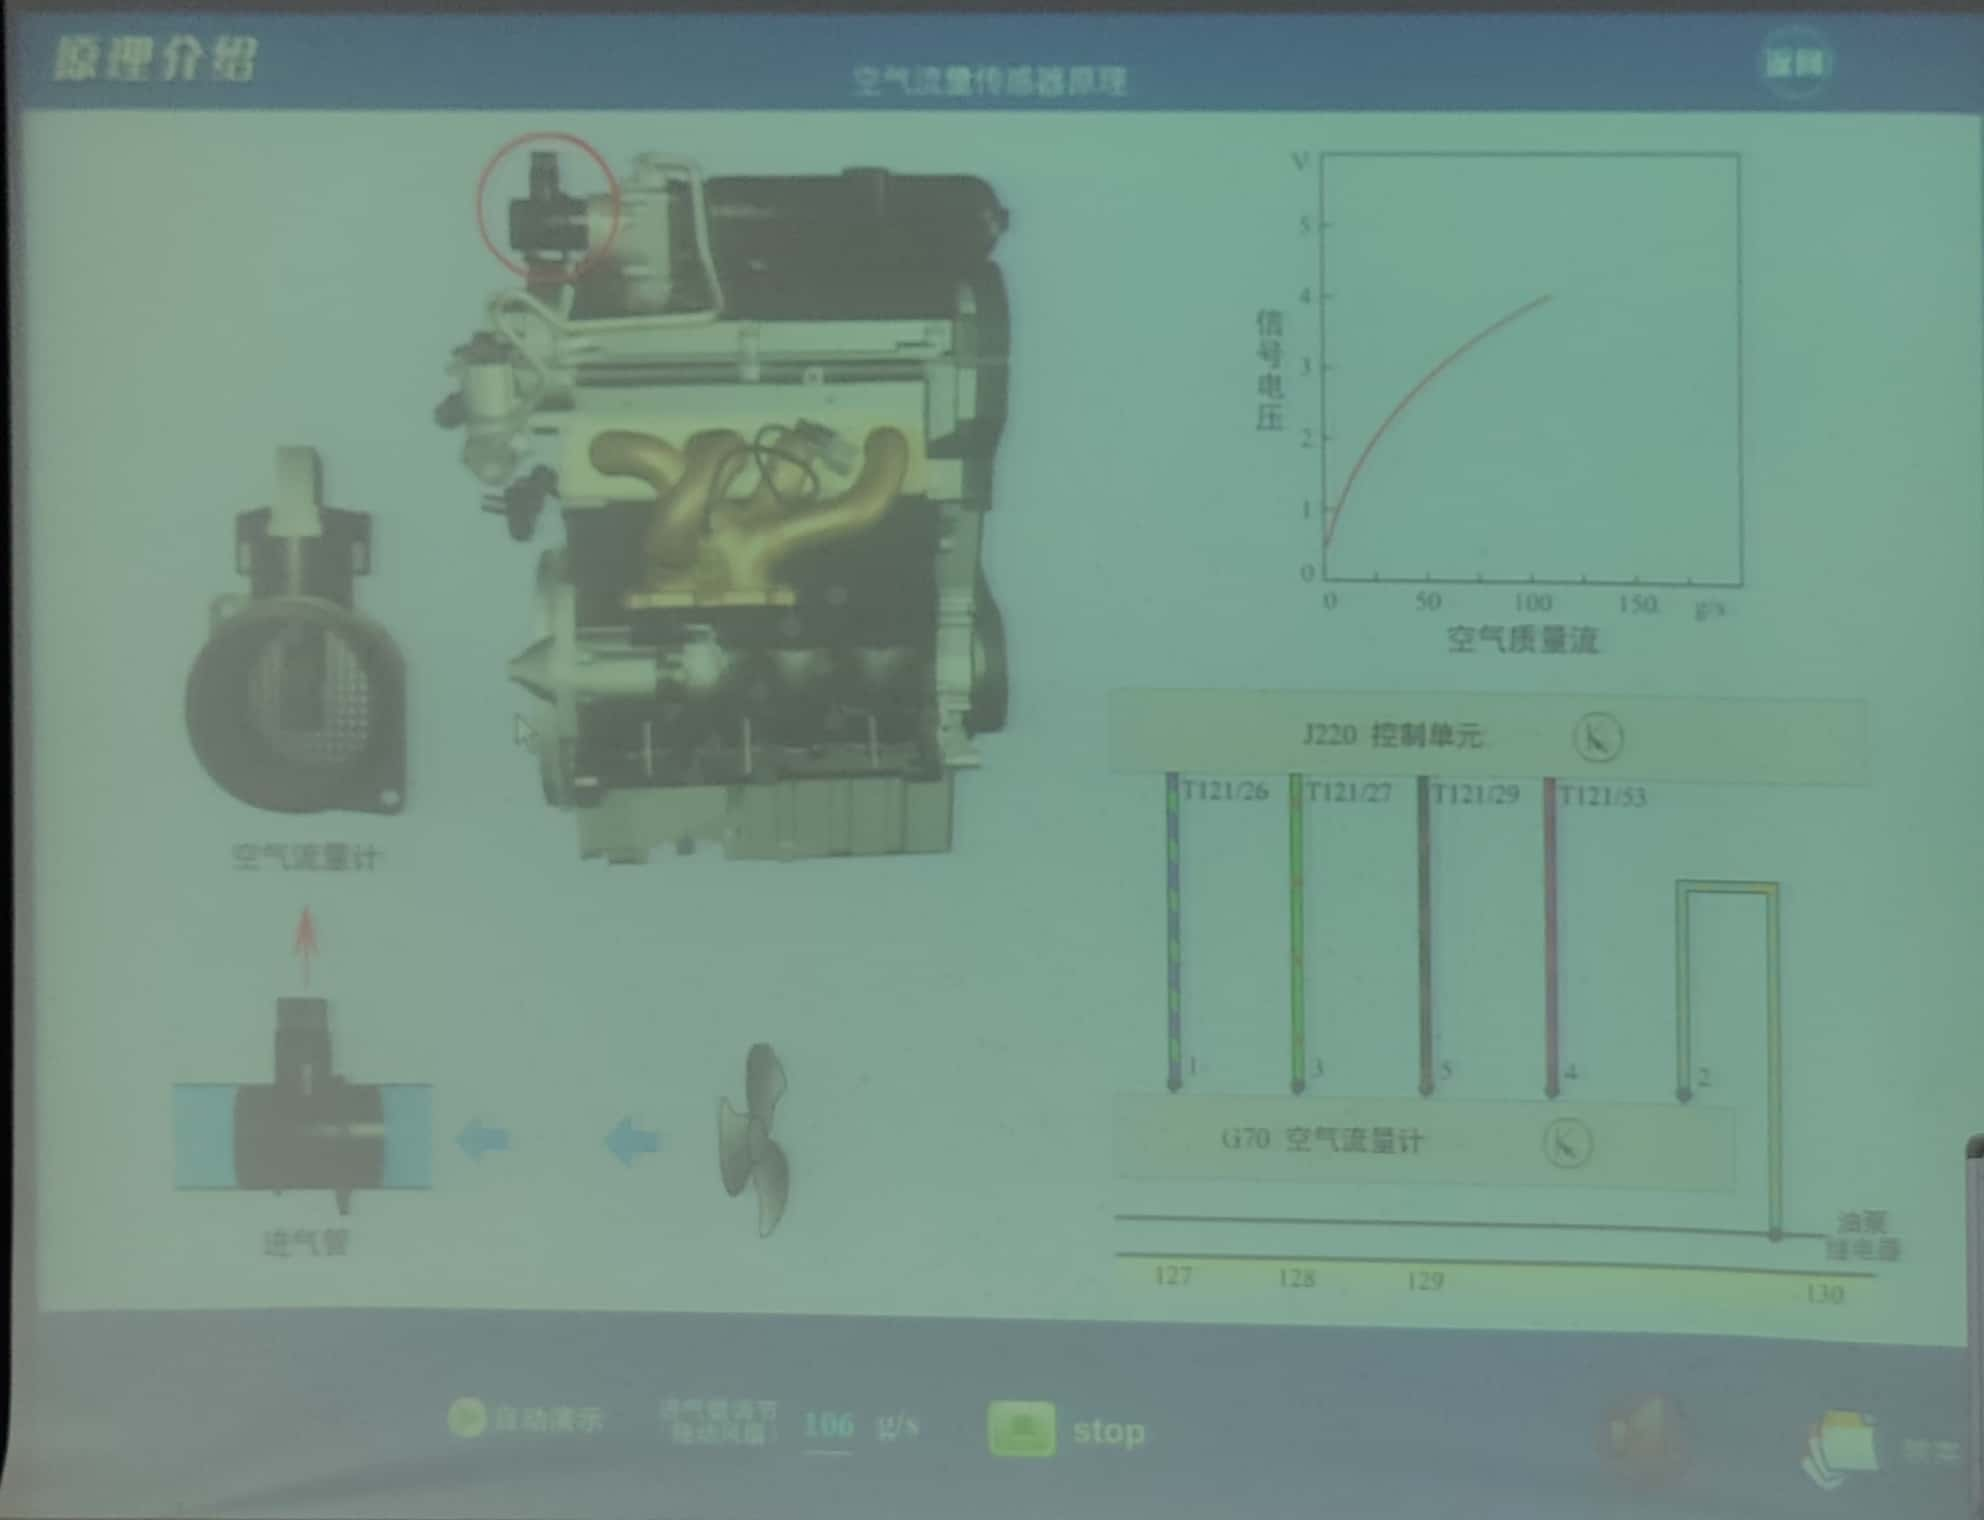
\includegraphics[width=0.45\textwidth]{airflowing sensor}\label{airflowing sensor}}
	\subfigure[前氧传感器]{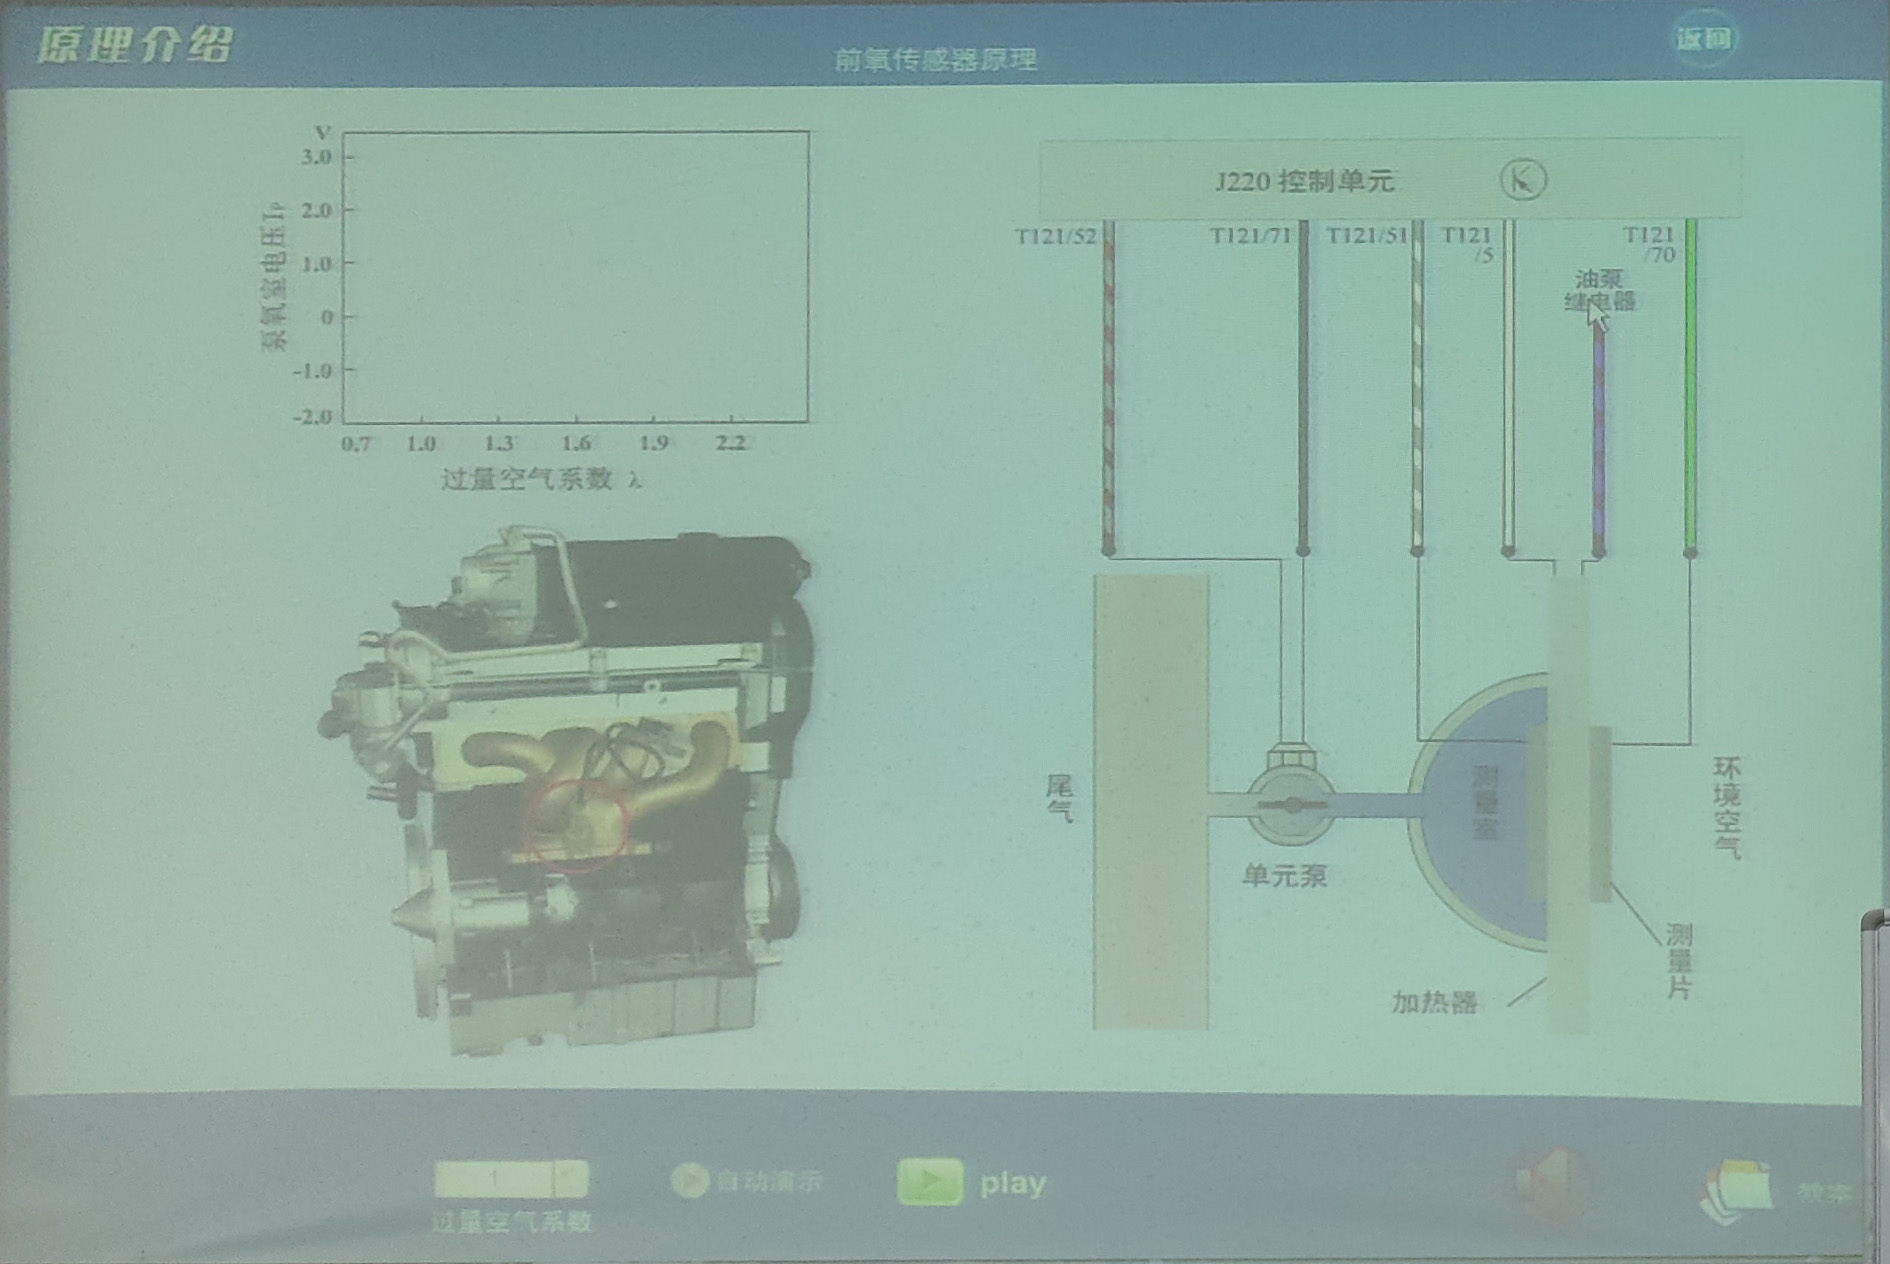
\includegraphics[width=0.45\textwidth]{oxygen sensor F}\label{oxygen sensor F}}
	\subfigure[后氧传感器]{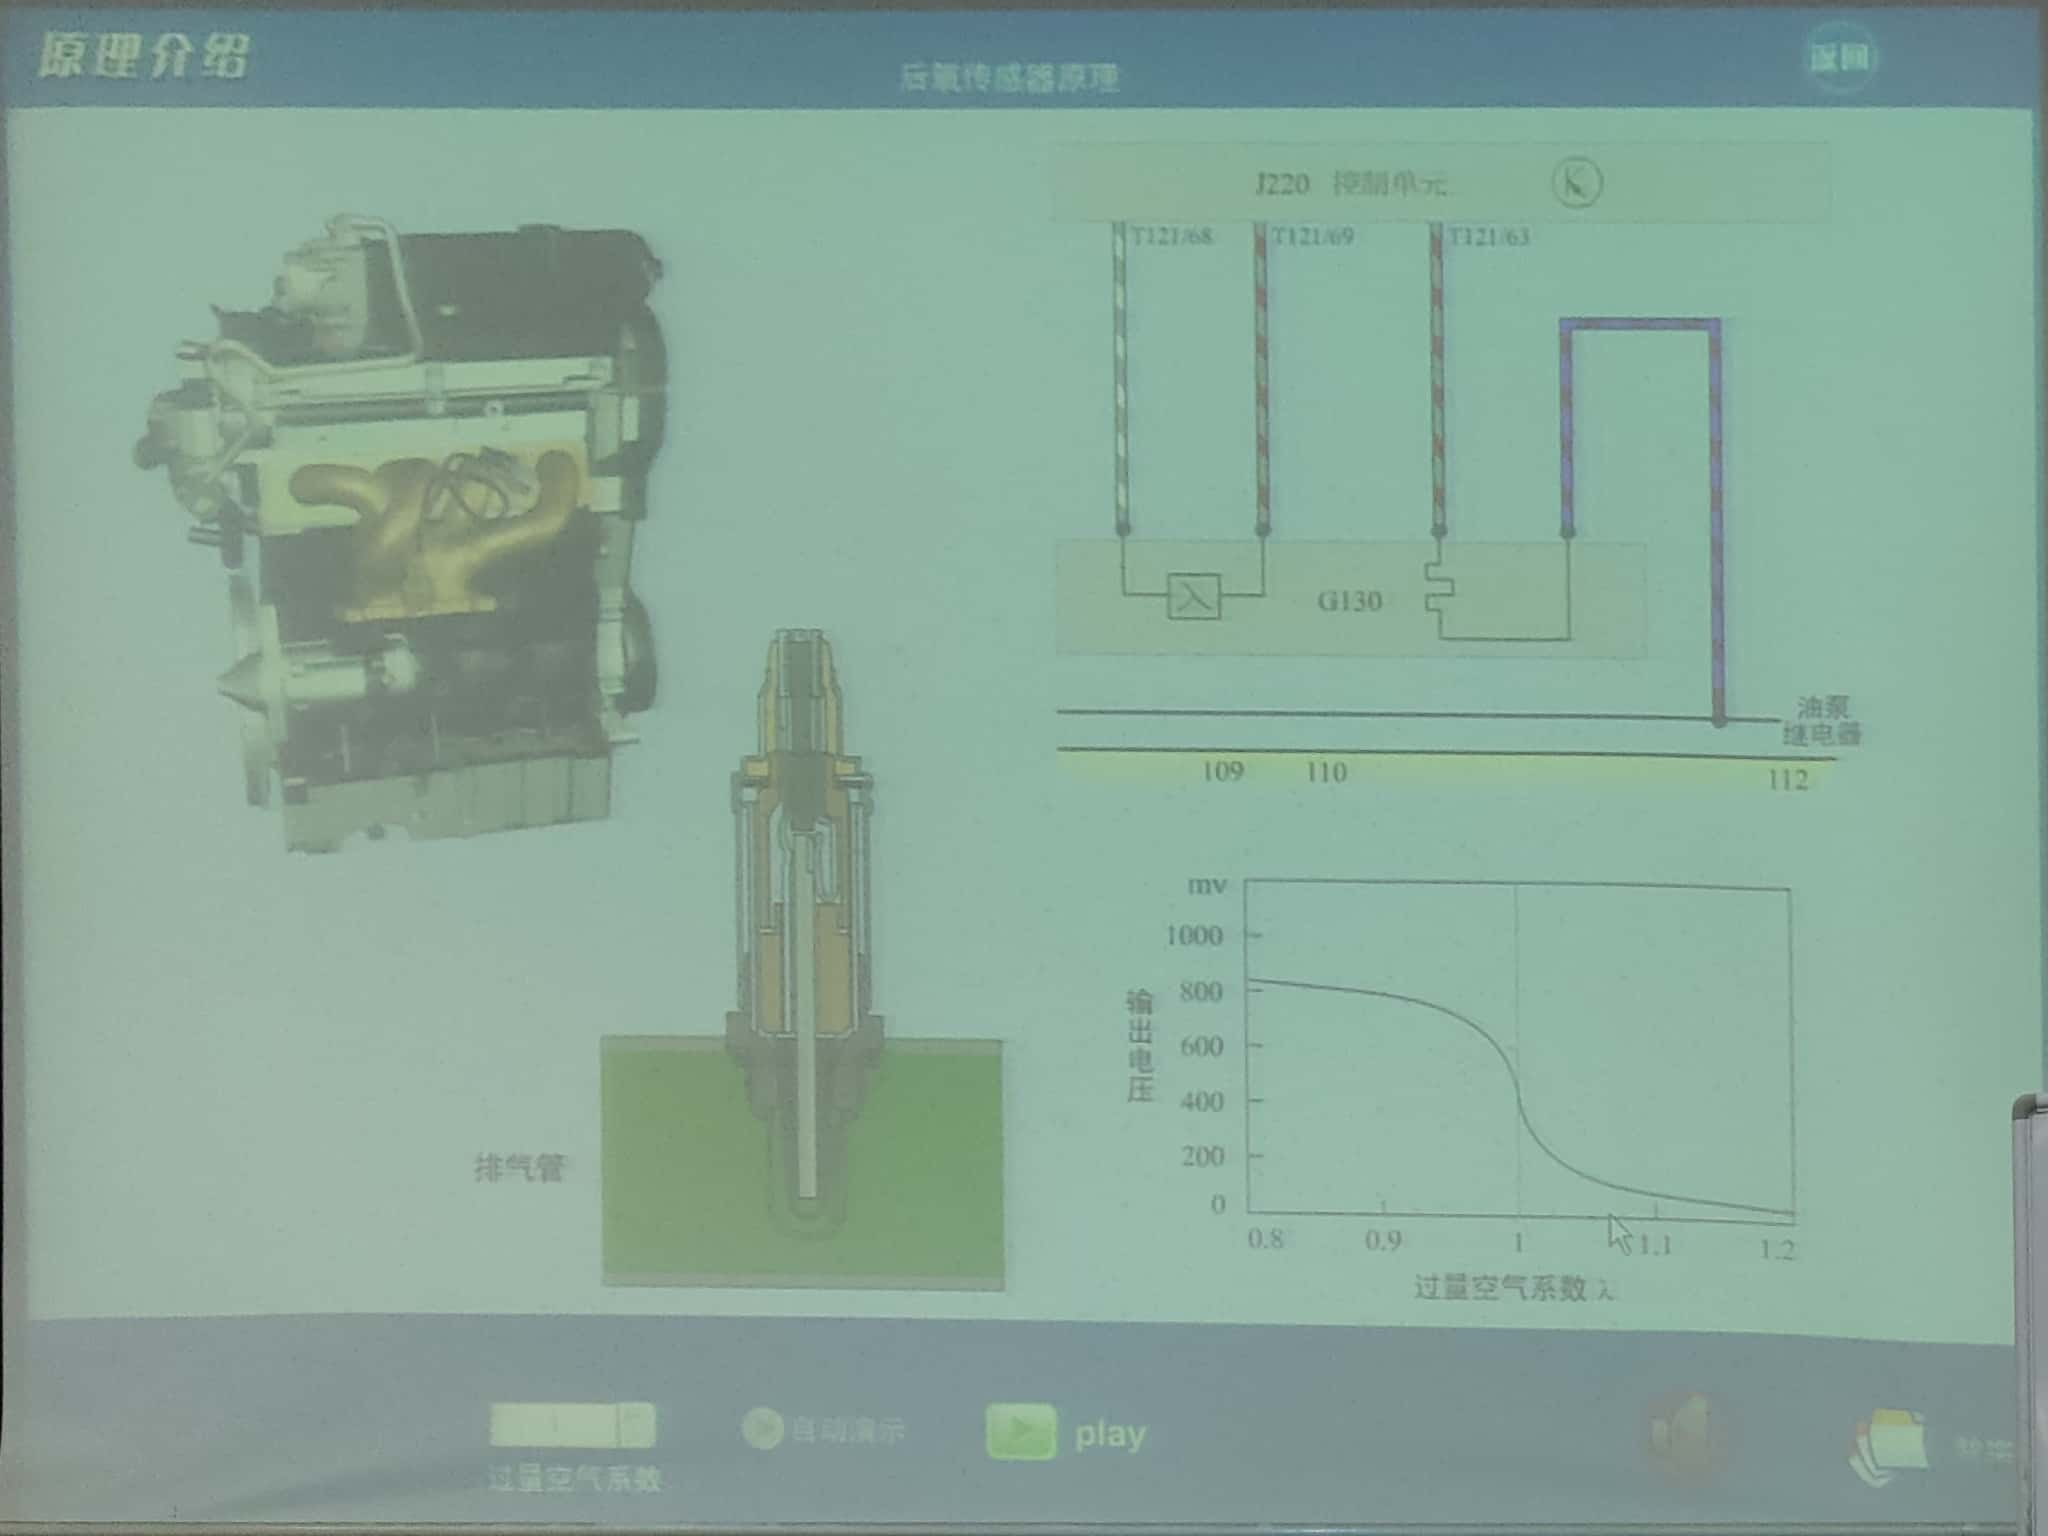
\includegraphics[width=0.45\textwidth]{oxygen sensor B}\label{oxygen sensor B}}
	\subfigure[冷却液温度传感器]{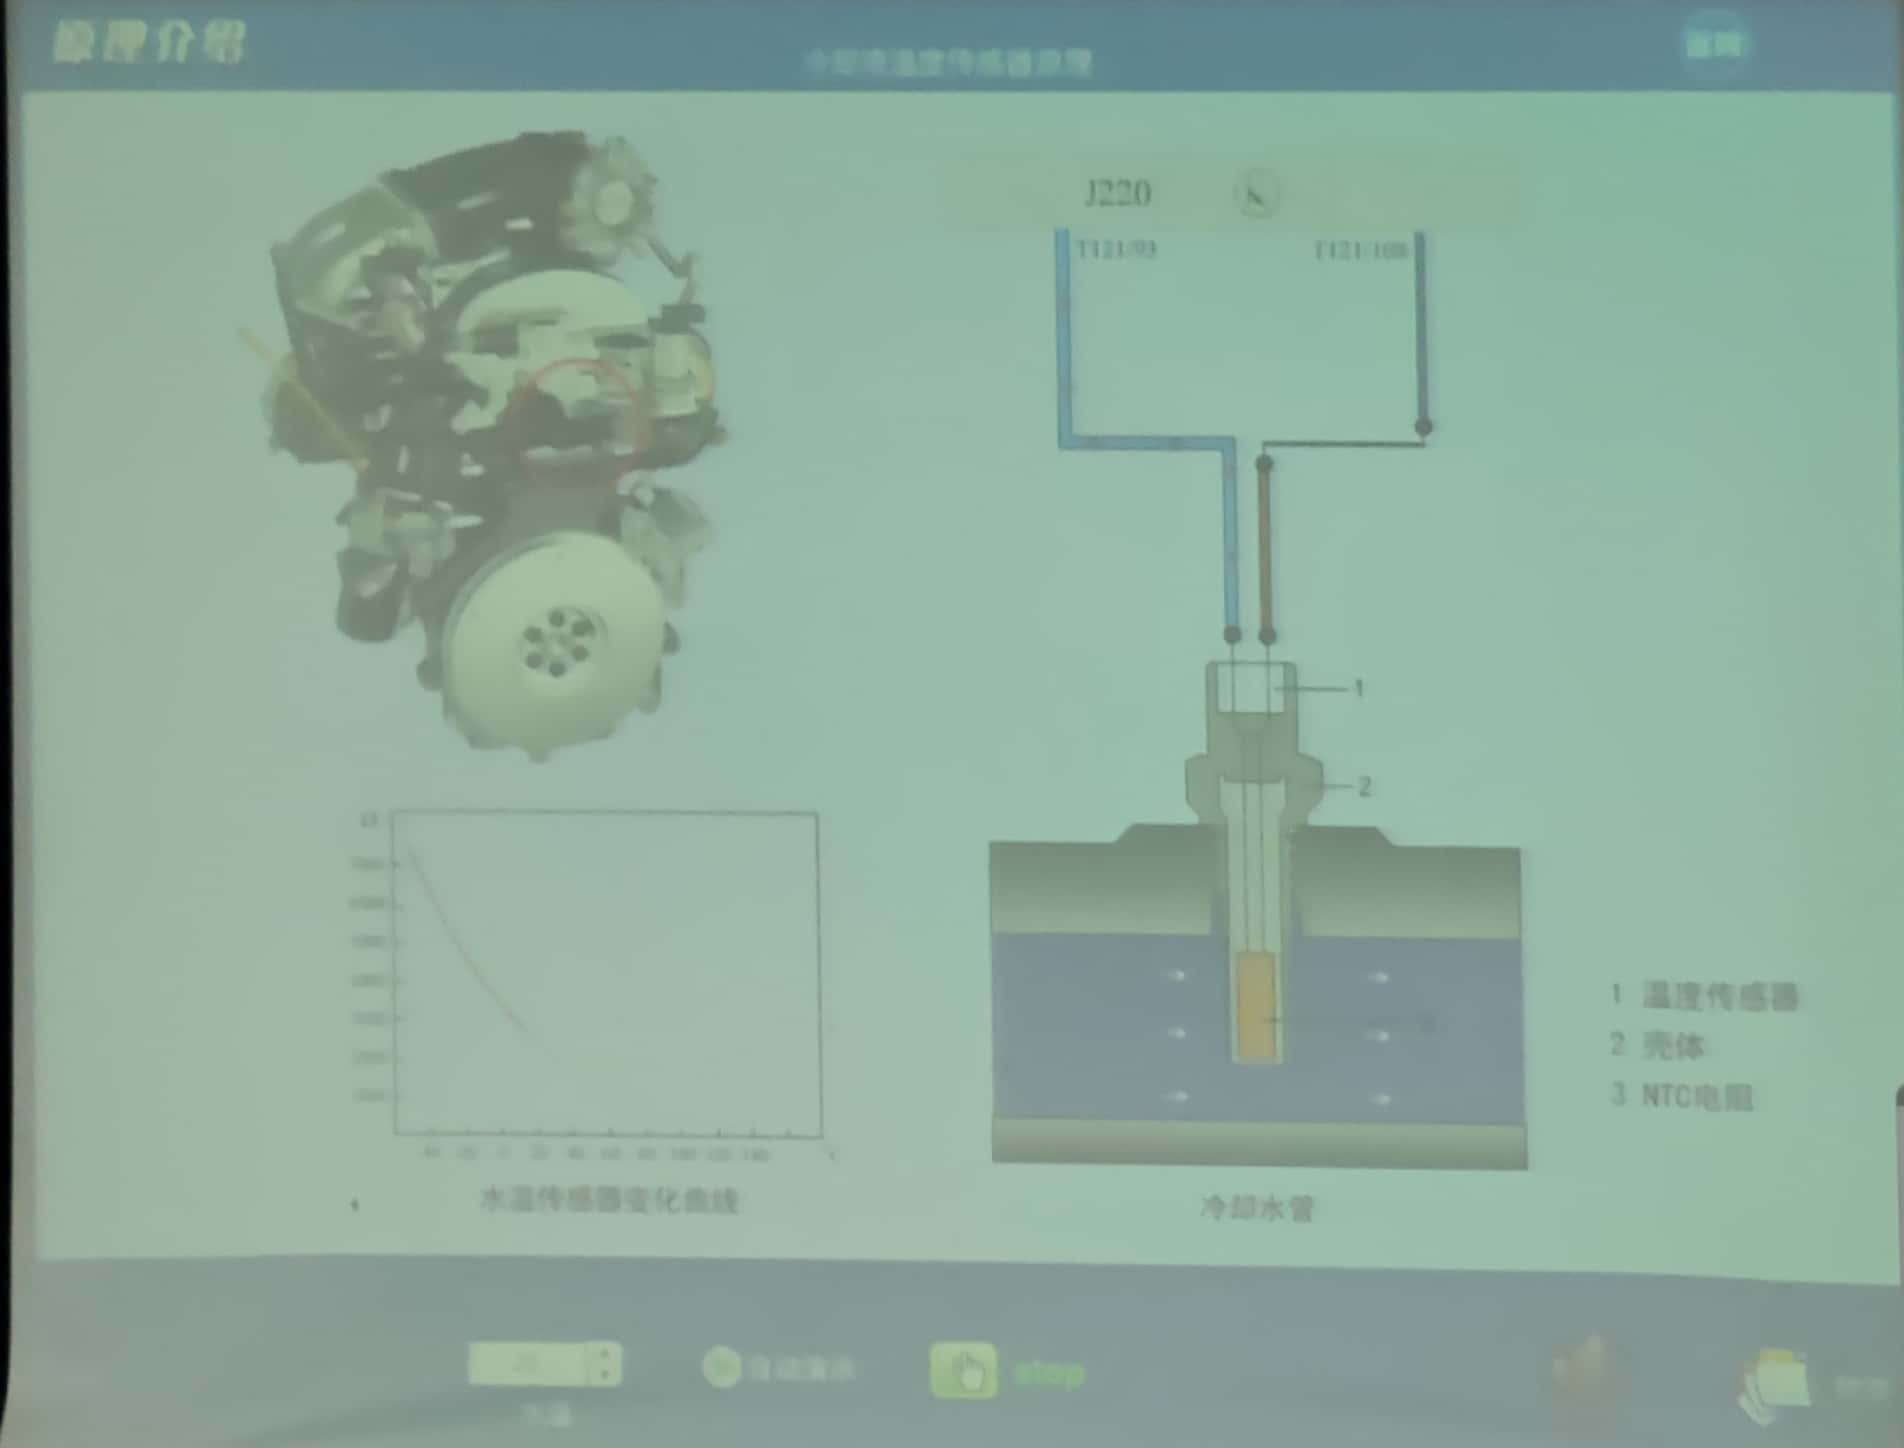
\includegraphics[width=0.45\textwidth]{coolant temperature sensor}\label{coolant temperature sensor}}
	\caption{发动机的控制系统中的部分传感器}
	\label{sensors}
\end{figure}

燃油泵继电器、燃油泵、喷油器、油箱等都是燃油供给系统(\cref{fuel-supplying system})的组成部分。对于缸内直喷汽油机,供油压力都很高,达到\qtyrange[range-phrase = $\,\sim\,$, range-units = single]{300}{450}{\kPa},需采用高压油轨,油轨中压力在发动机运转时变化不大,ECU对喷油器的控制主要是控制其喷油时刻和喷油持续时间。燃油泵继电器只在起动时和发动机运转时接通电动燃油泵,提供足够的燃油压力和富余燃油;当发动机发生事故而停止运转时,燃油泵也停止运转,降低起火风险。油箱内因汽油蒸发产生的高压蒸气通到炭罐(\cref{charcoal canister})中,炭罐底部接大气,上部一边接油箱一边接进气管,ECU在需要时开启炭罐控制阀,燃油蒸气在压力差的作用下被导入到进气管中,随后进入气缸中燃烧。当然,炭罐系统的存在也使得燃油供给量不完全由喷油量控制,且经过炭罐的蒸气量不便计量,这也是需要设置氧传感器进行$\lambda$闭环控制的原因之一。

点火系统要能保证按时并提供足量能量点燃燃烧室内混合气。最佳点火提前角受很多因素影响,其中最主要的是发动机转速和混合气的燃烧速度,而混合气的燃烧速度又和混合气的成分、发动机的结构(包括燃烧室形状和压缩比)等有关。当发动机转速一定时,随着负荷(节气门开度)的增加,进入气缸的可燃混合气增多,压缩终了时的压力和温度升高,同时残余废气在缸内混合气中所占的比例下降,混合气燃烧速度增大,点火提前角应适当减小;反之负荷减小时点火提前角应加大。当节气门开度一定时,发动机转速升高,燃烧过程所占曲轴转角增大,应适当加大点火提前角,否则燃烧会延续到做功冲程使得功率和经济性下降。对于抗爆性较好的汽油,许用的点火提前角较大,加注不同牌号的汽油后点火提前角也应相应调节。ECU确定点火提前角后,发出信号令点火系统点火。电控点火系统分为有分电器式和无分电器式两种,现在用的多为无分电器点火系统,又称直接点火系统。直接点火系统又有单火花点火线圈、双火花点火线圈和四火花点火线圈等,\cref{ignition system}所示为双火花点火线圈,1、4缸和2、3缸分别同时点火,这样点火时一个气缸在压缩冲程的上止点附近,另一个气缸运行到排气冲程上止点附近,但只有一个缸中有可燃混合气,可以被点燃。

\cref{VVT}所示的是一种张紧轮式进气相位调节装置,排气凸轮相位固定,液压缸使链条的上(下)部分张紧且长度发生变化,从而带动进气凸轮相对旋转一角度实现可变气门正时。怠速时,进气门延迟关闭,改善燃烧稳定性;中、低转速时,进气门提前关闭,以获得较大转矩;高转速时,进气门延迟关闭,利用进气惯性提高气缸充气量以提高功率。

在电子节气门系统(\cref{electronic throttle})中,节气门与加速踏板间无拉索的机械连接,节气门开度完全受ECU控制。当发动机不运转且点火开关打开时,ECU只根据加速踏板位置控制节气门控制器。当发动机运转时,ECU对节气门的控制不完全依赖加速踏板的输入,譬如说可在加速踏板仅踏下一半时即令节气门全开,减少节流损失。有电子节气门的发动机还不需怠速调节器,进气量可精确控制,在提升车辆驾驶性能的同时降低排放和油耗。

二次空气系统(\cref{secondary air})和排气再循环系统(\cref{EGR})都是发动机排放控制系统的一部分,现代发动机管理系统将喷油控制和排放控制作为统一的整体,以满足日趋严格的排放法规。二次空气系统主要在发动机冷起动和暖机过程中工作,在每缸排气门后面导入空气,使得高温废气中的\ce{HC}和\ce{CO}在排气管中继续燃烧,产生热量让催化转换器尽快升温。排气再循环系统通过回引部分废气与新鲜空气一起参与燃烧,降低混合气中\ce{O2}含量和燃烧温度从而抑制\ce{NO_x}的产生。

正如\cref{subsection:1.1}所提到的那样,废气涡轮增压系统(\cref{turbocharging})上的放气阀也受ECU控制。

\begin{figure}[htbp]
	\centering
	\subfigure[燃油供给系统]{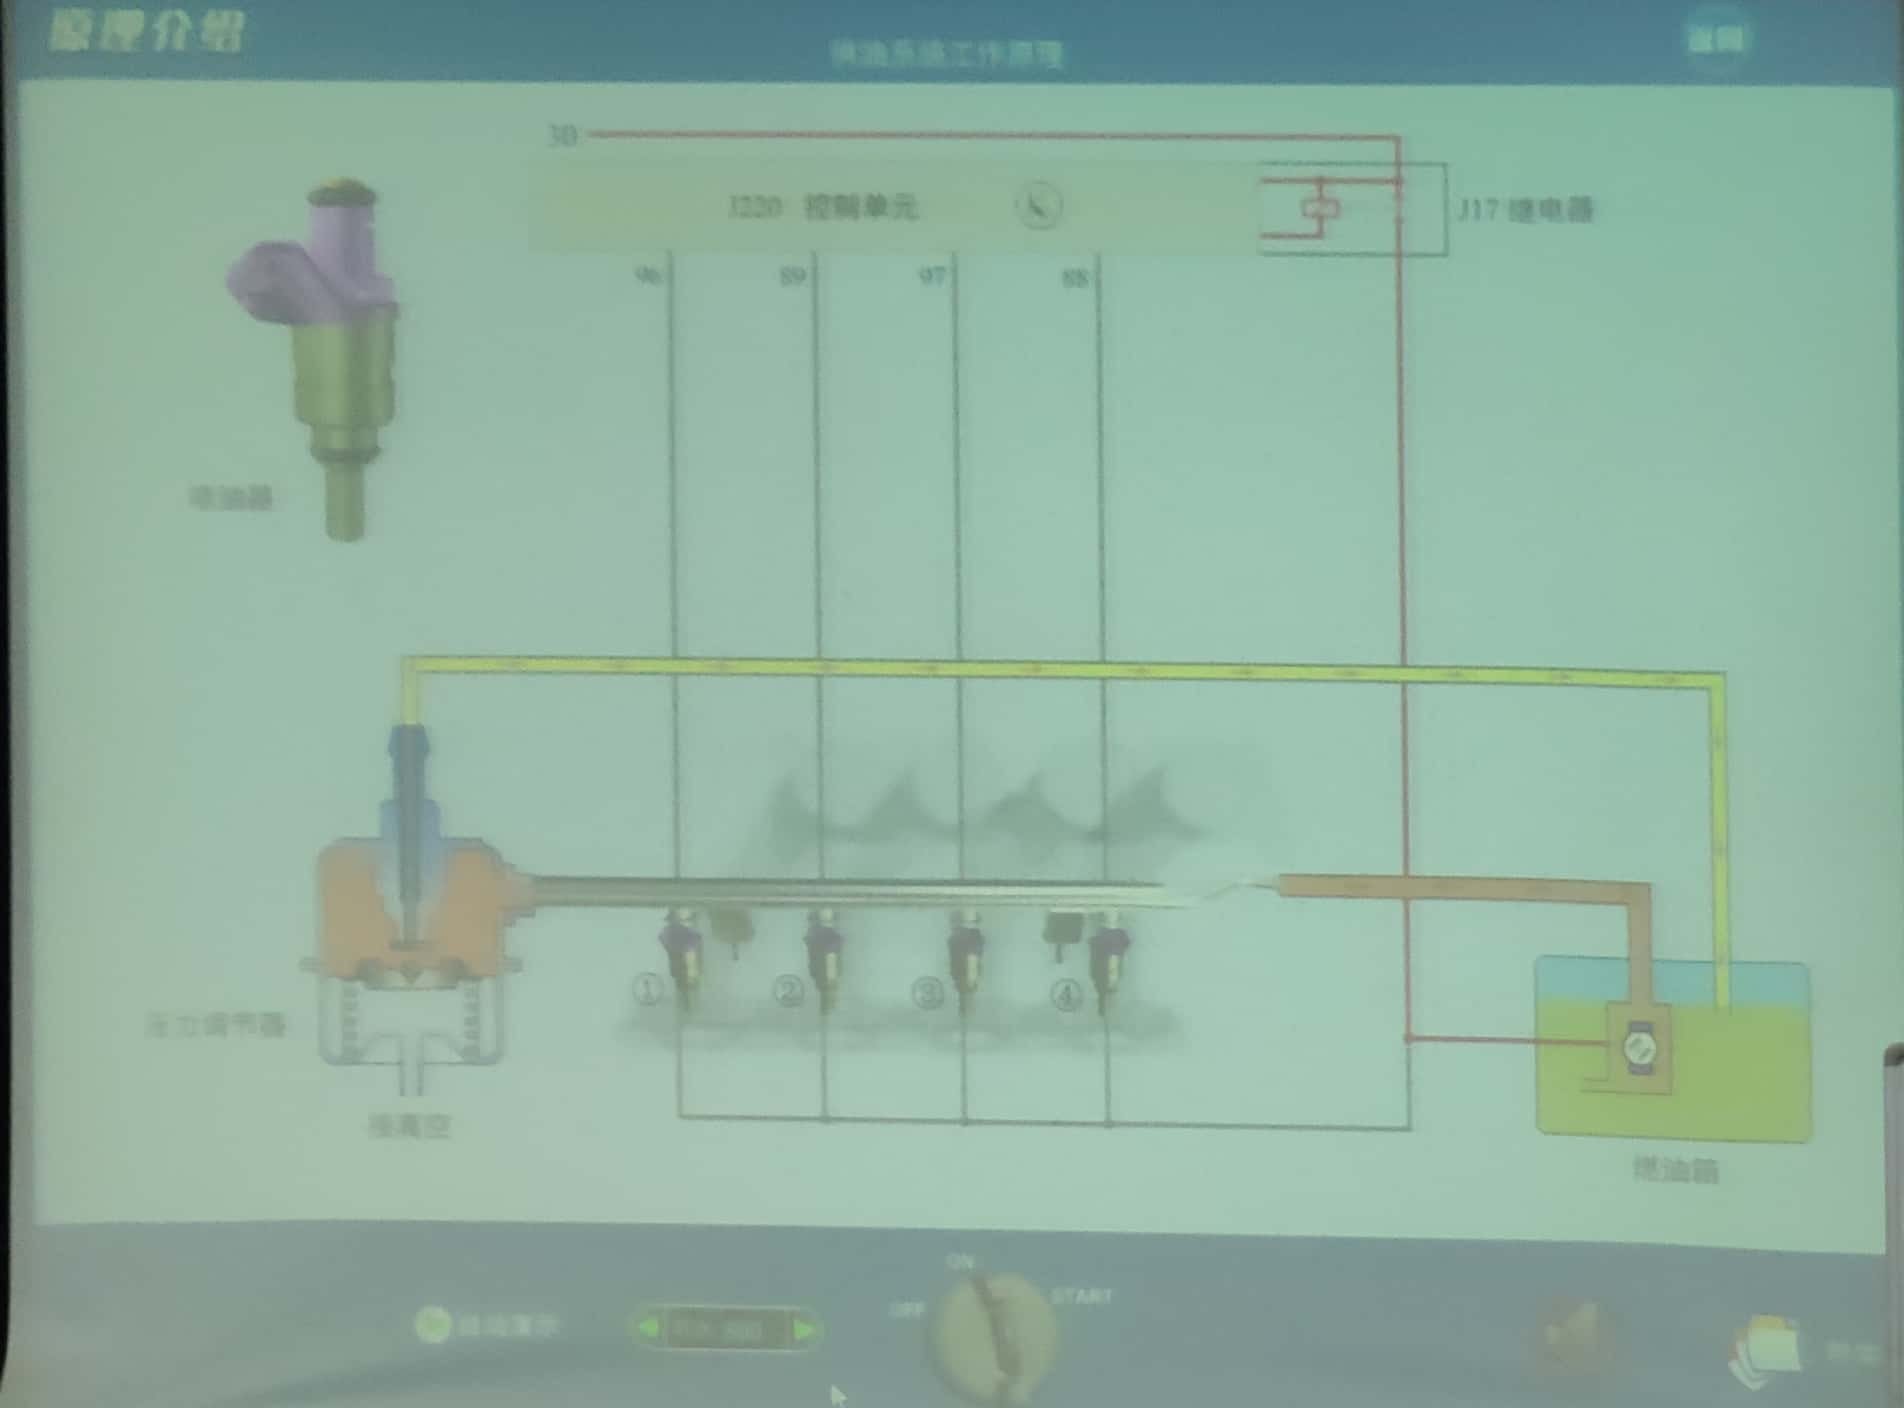
\includegraphics[width=0.3\textwidth]{fuel-supplying system}\label{fuel-supplying system}}
	\subfigure[炭罐]{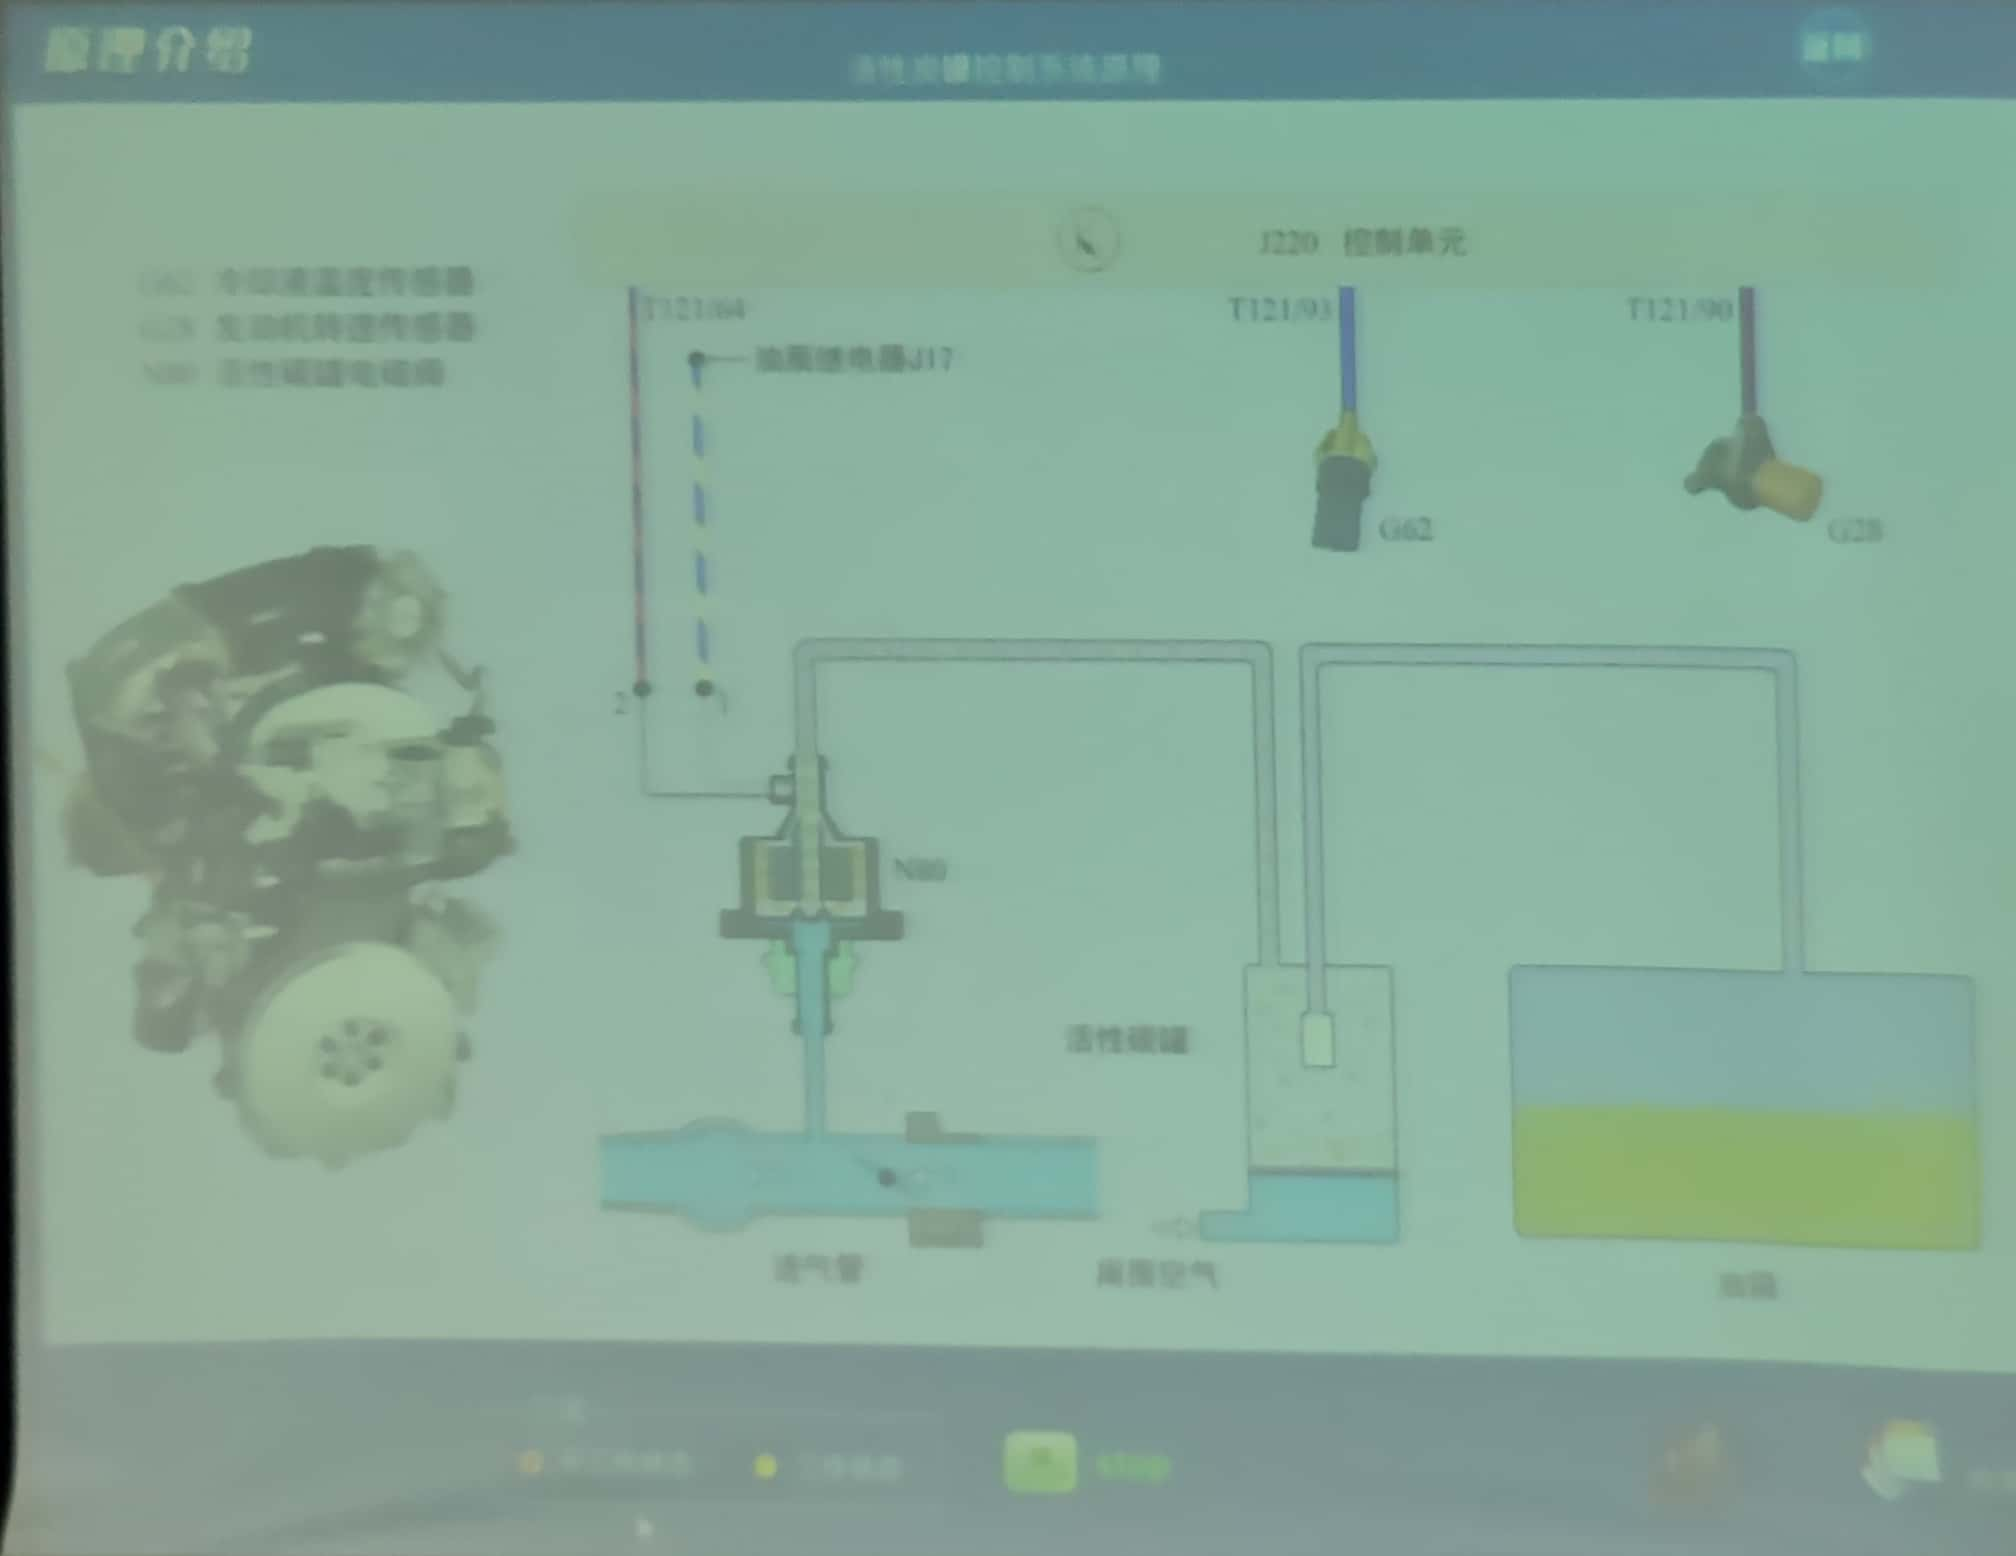
\includegraphics[width=0.3\textwidth]{charcoal canister}\label{charcoal canister}}
	\subfigure[点火系统]{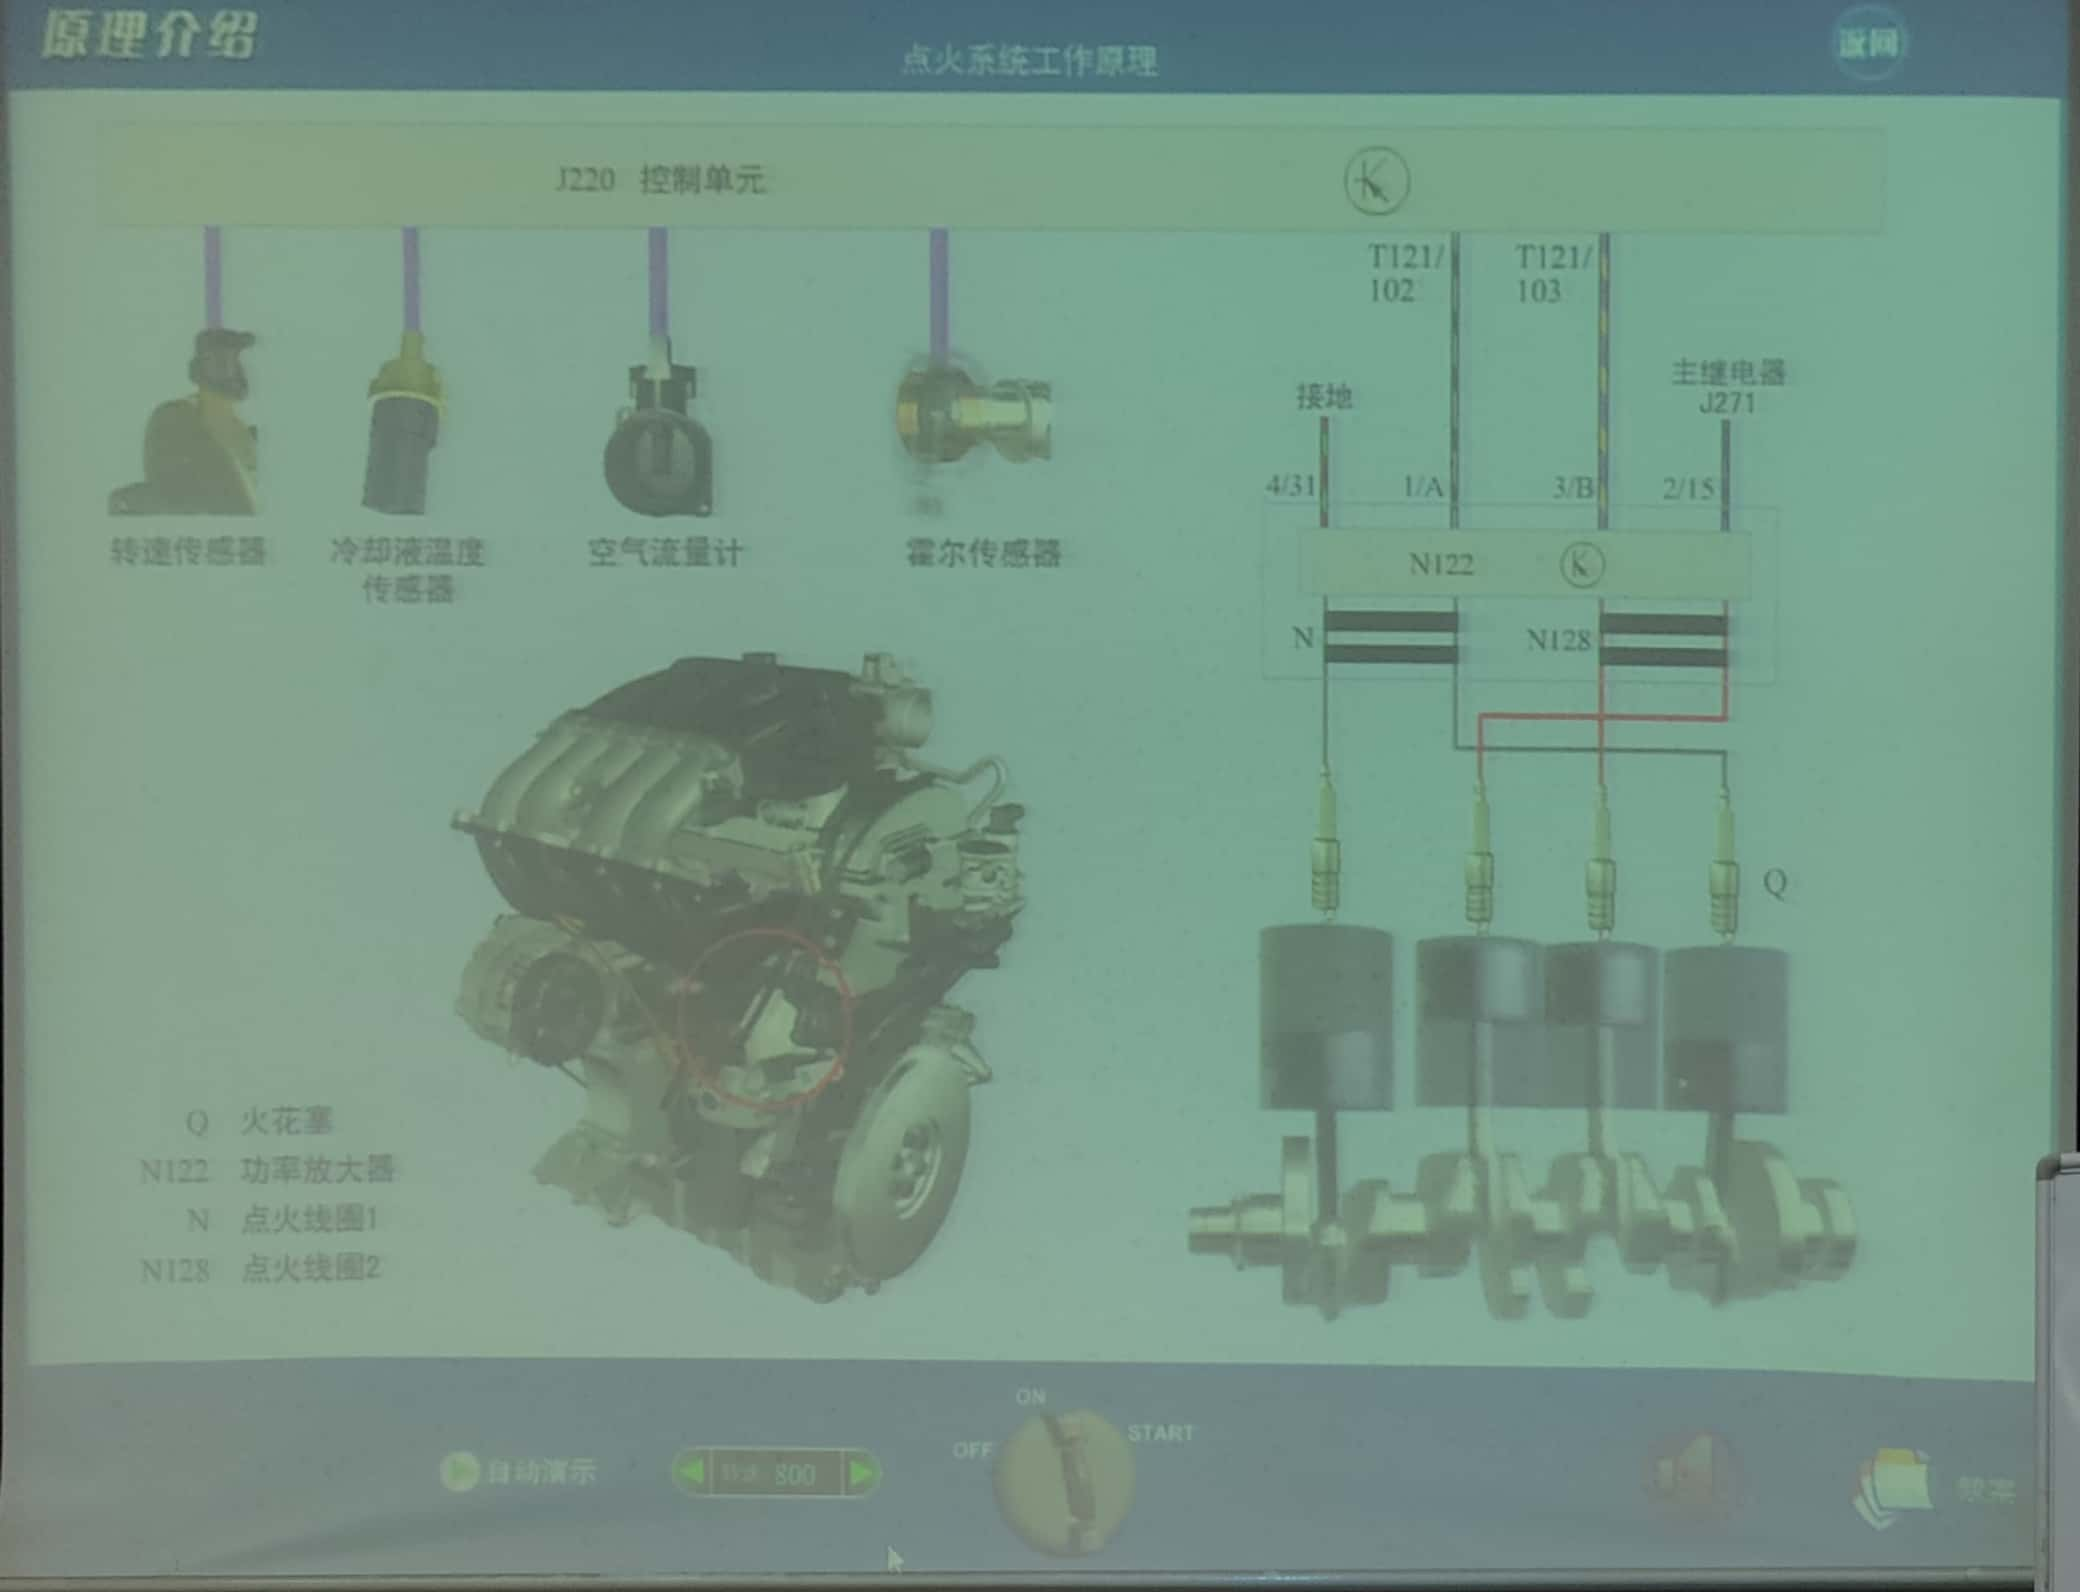
\includegraphics[width=0.3\textwidth]{ignition system}\label{ignition system}}
	\subfigure[可变气门正时]{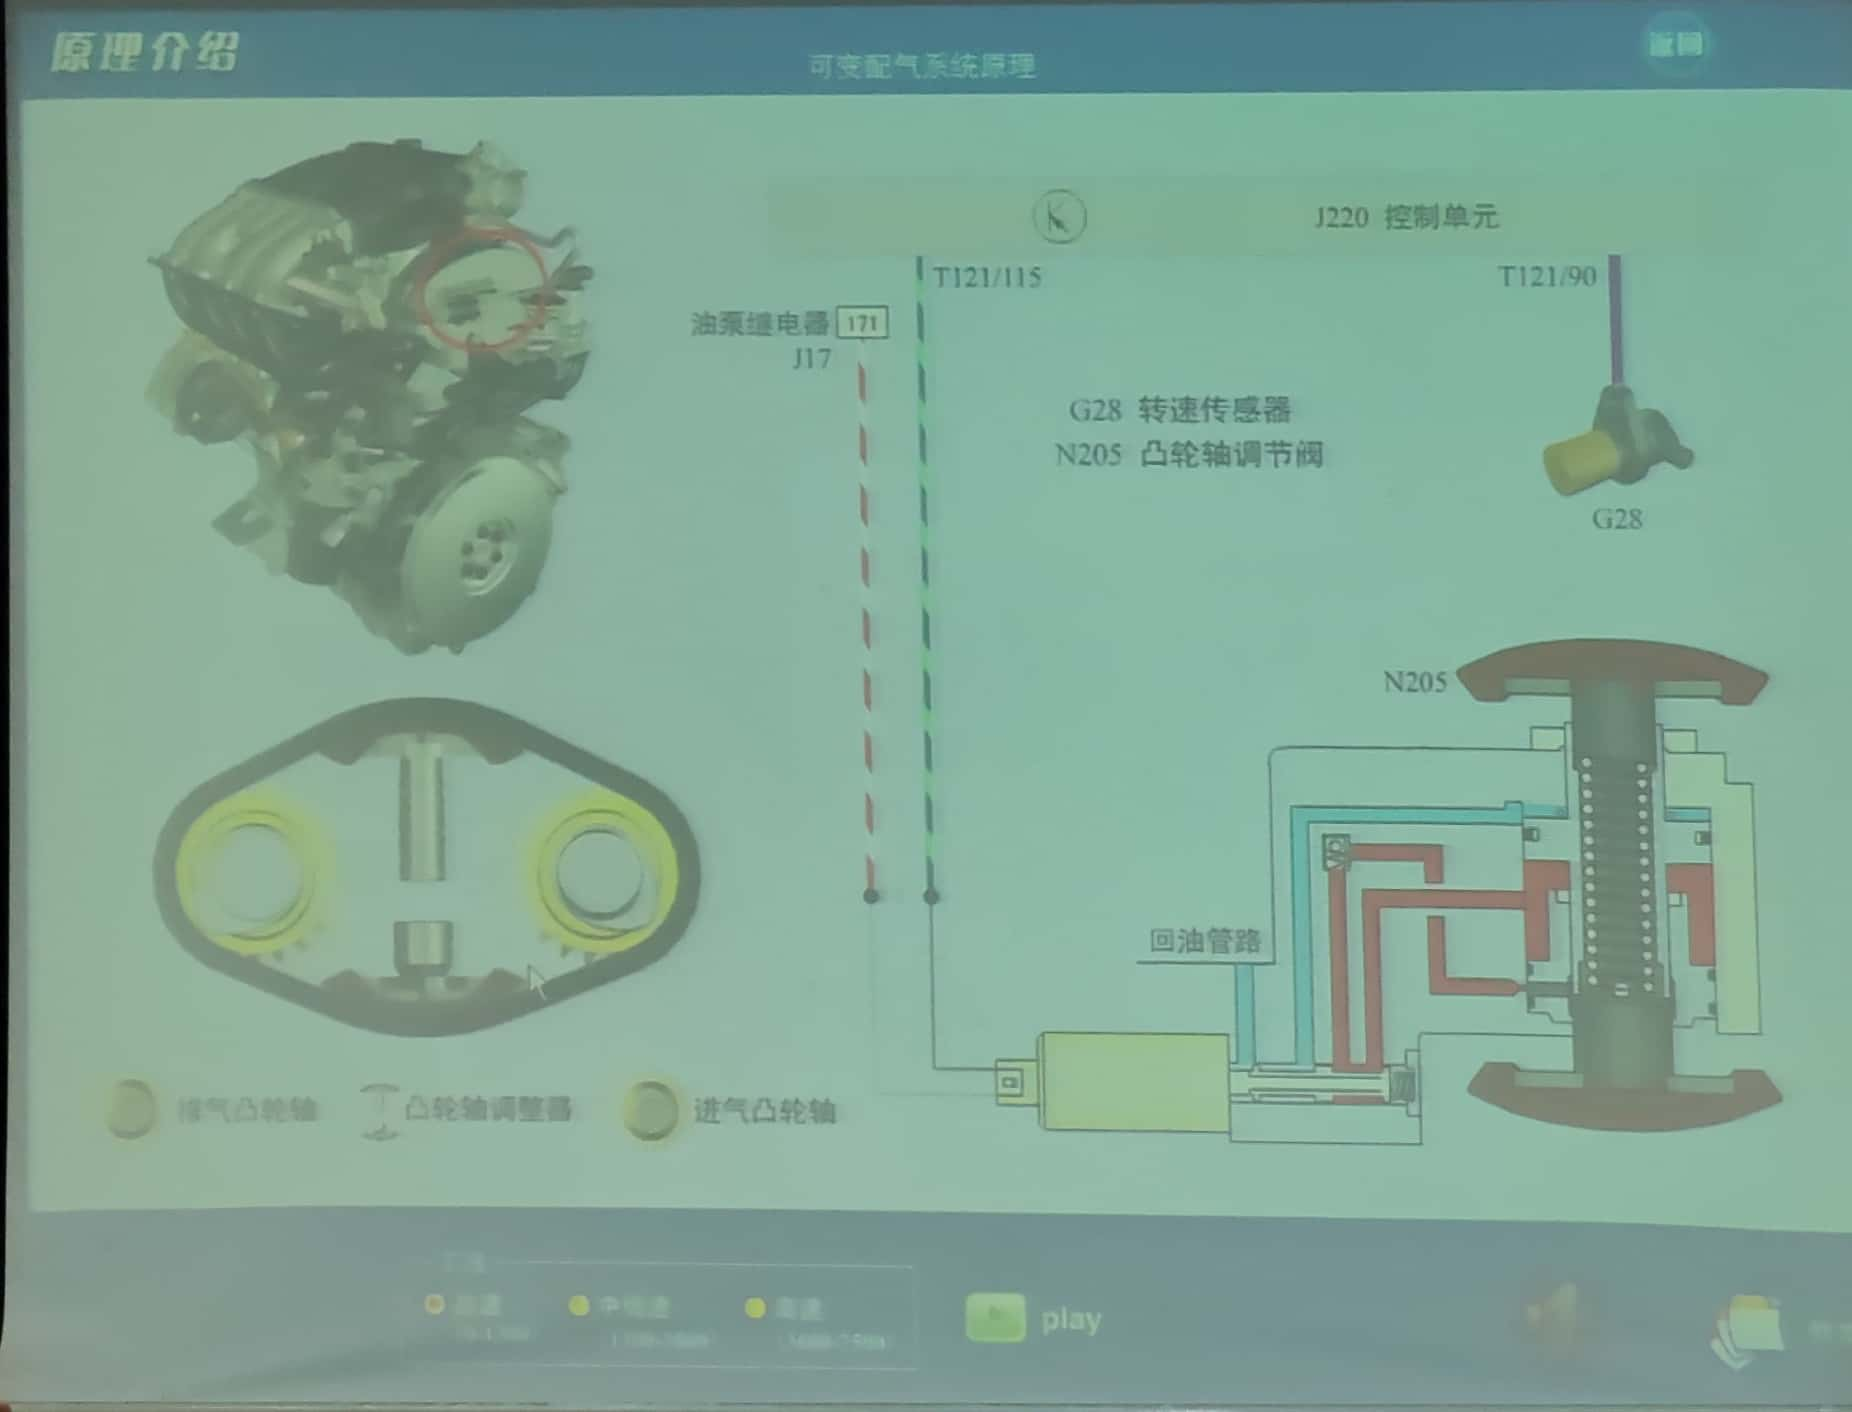
\includegraphics[width=0.3\textwidth]{VVT}\label{VVT}}
	\subfigure[电子油门]{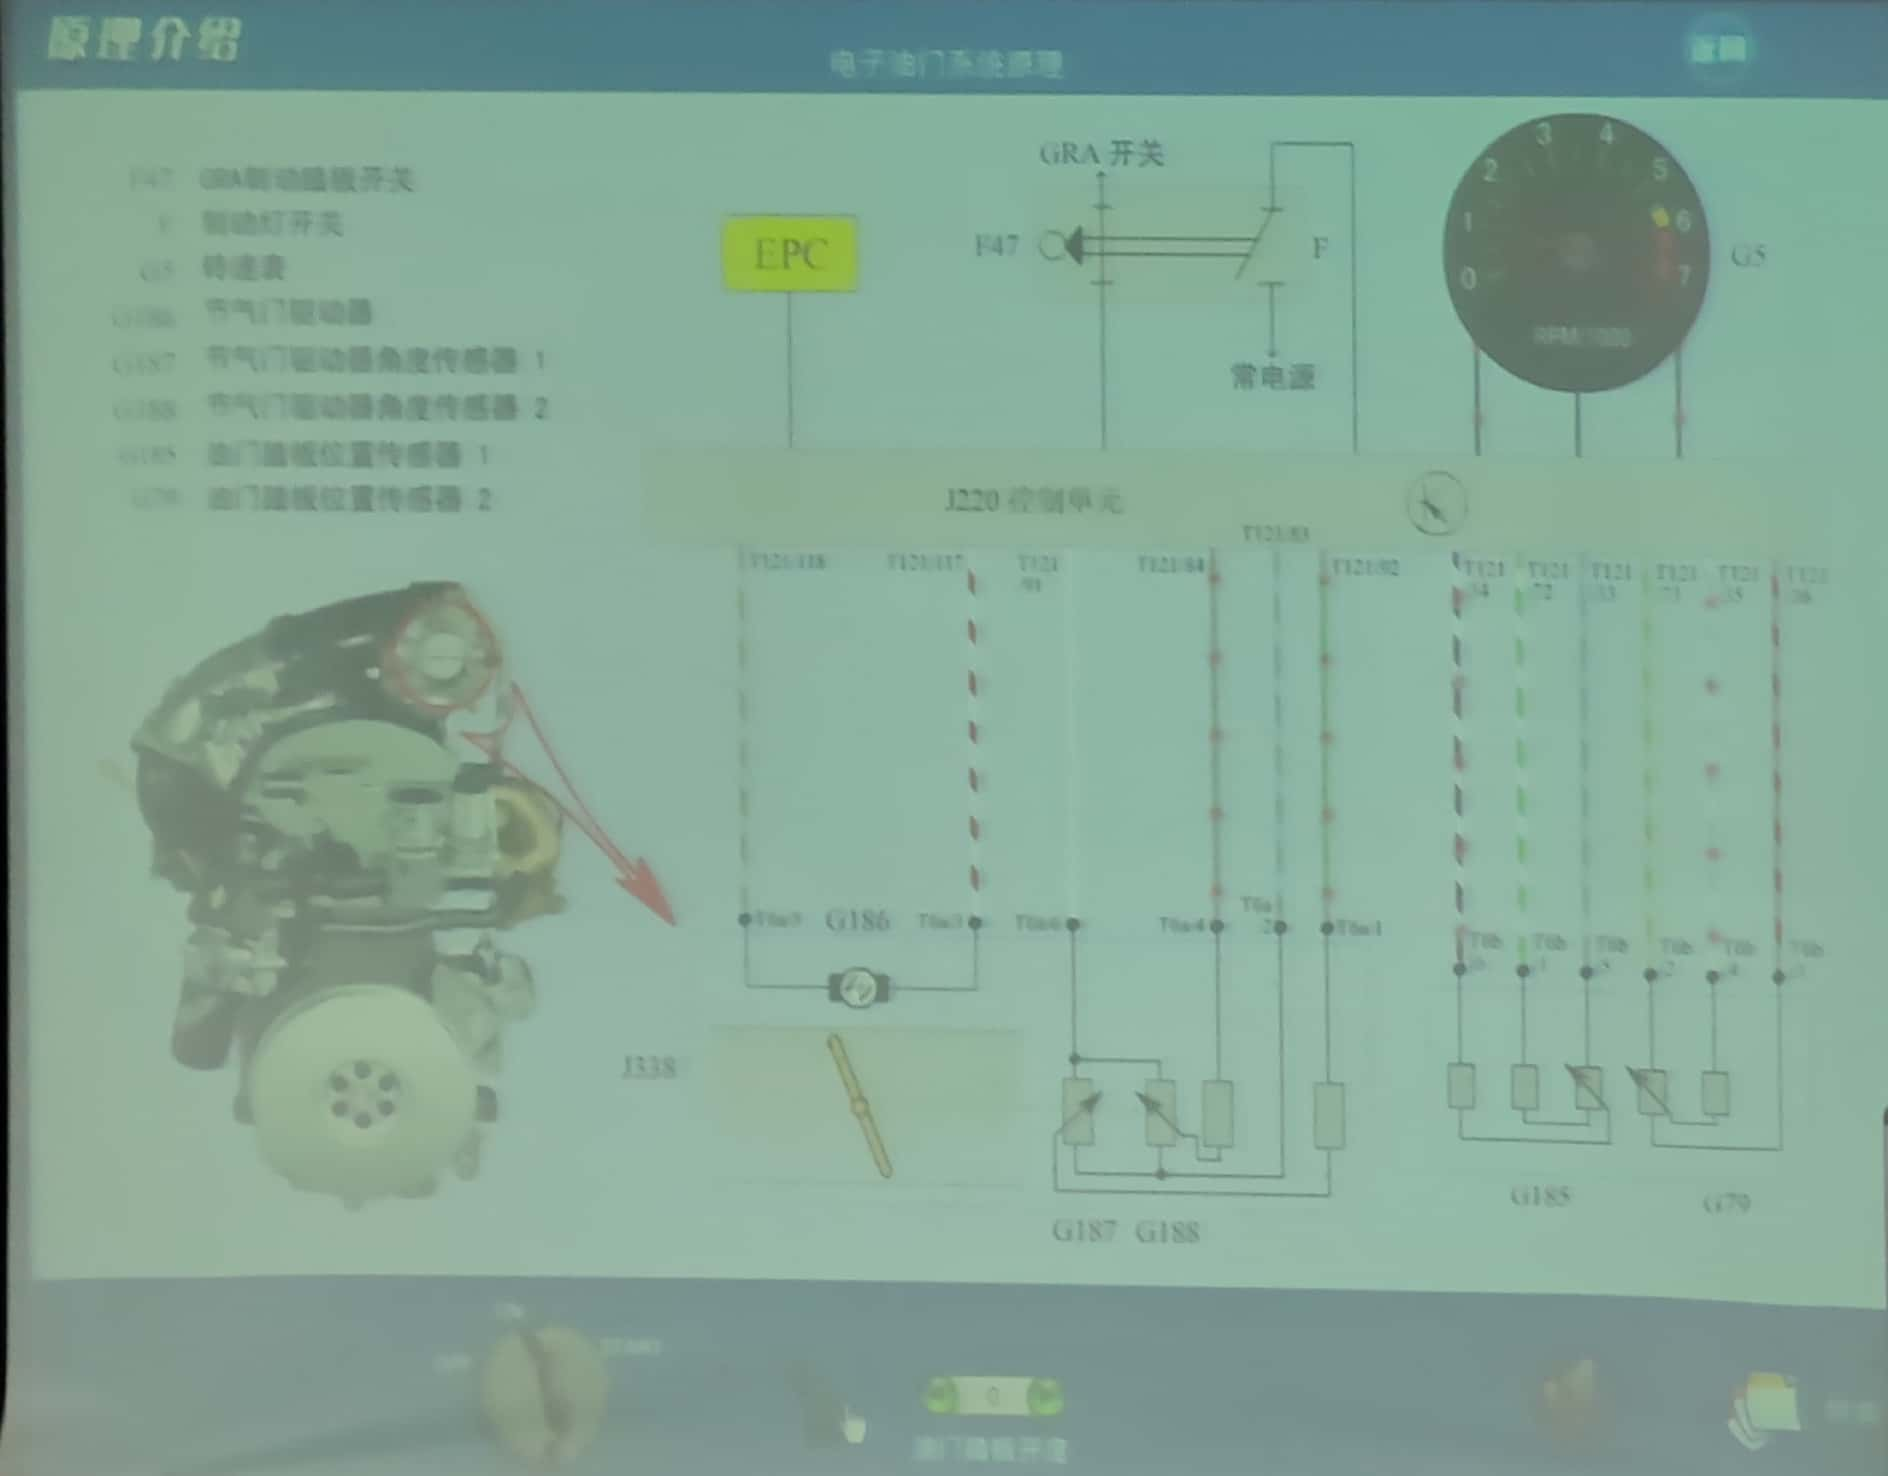
\includegraphics[width=0.3\textwidth]{electronic throttle}\label{electronic throttle}}
	\subfigure[二次空气]{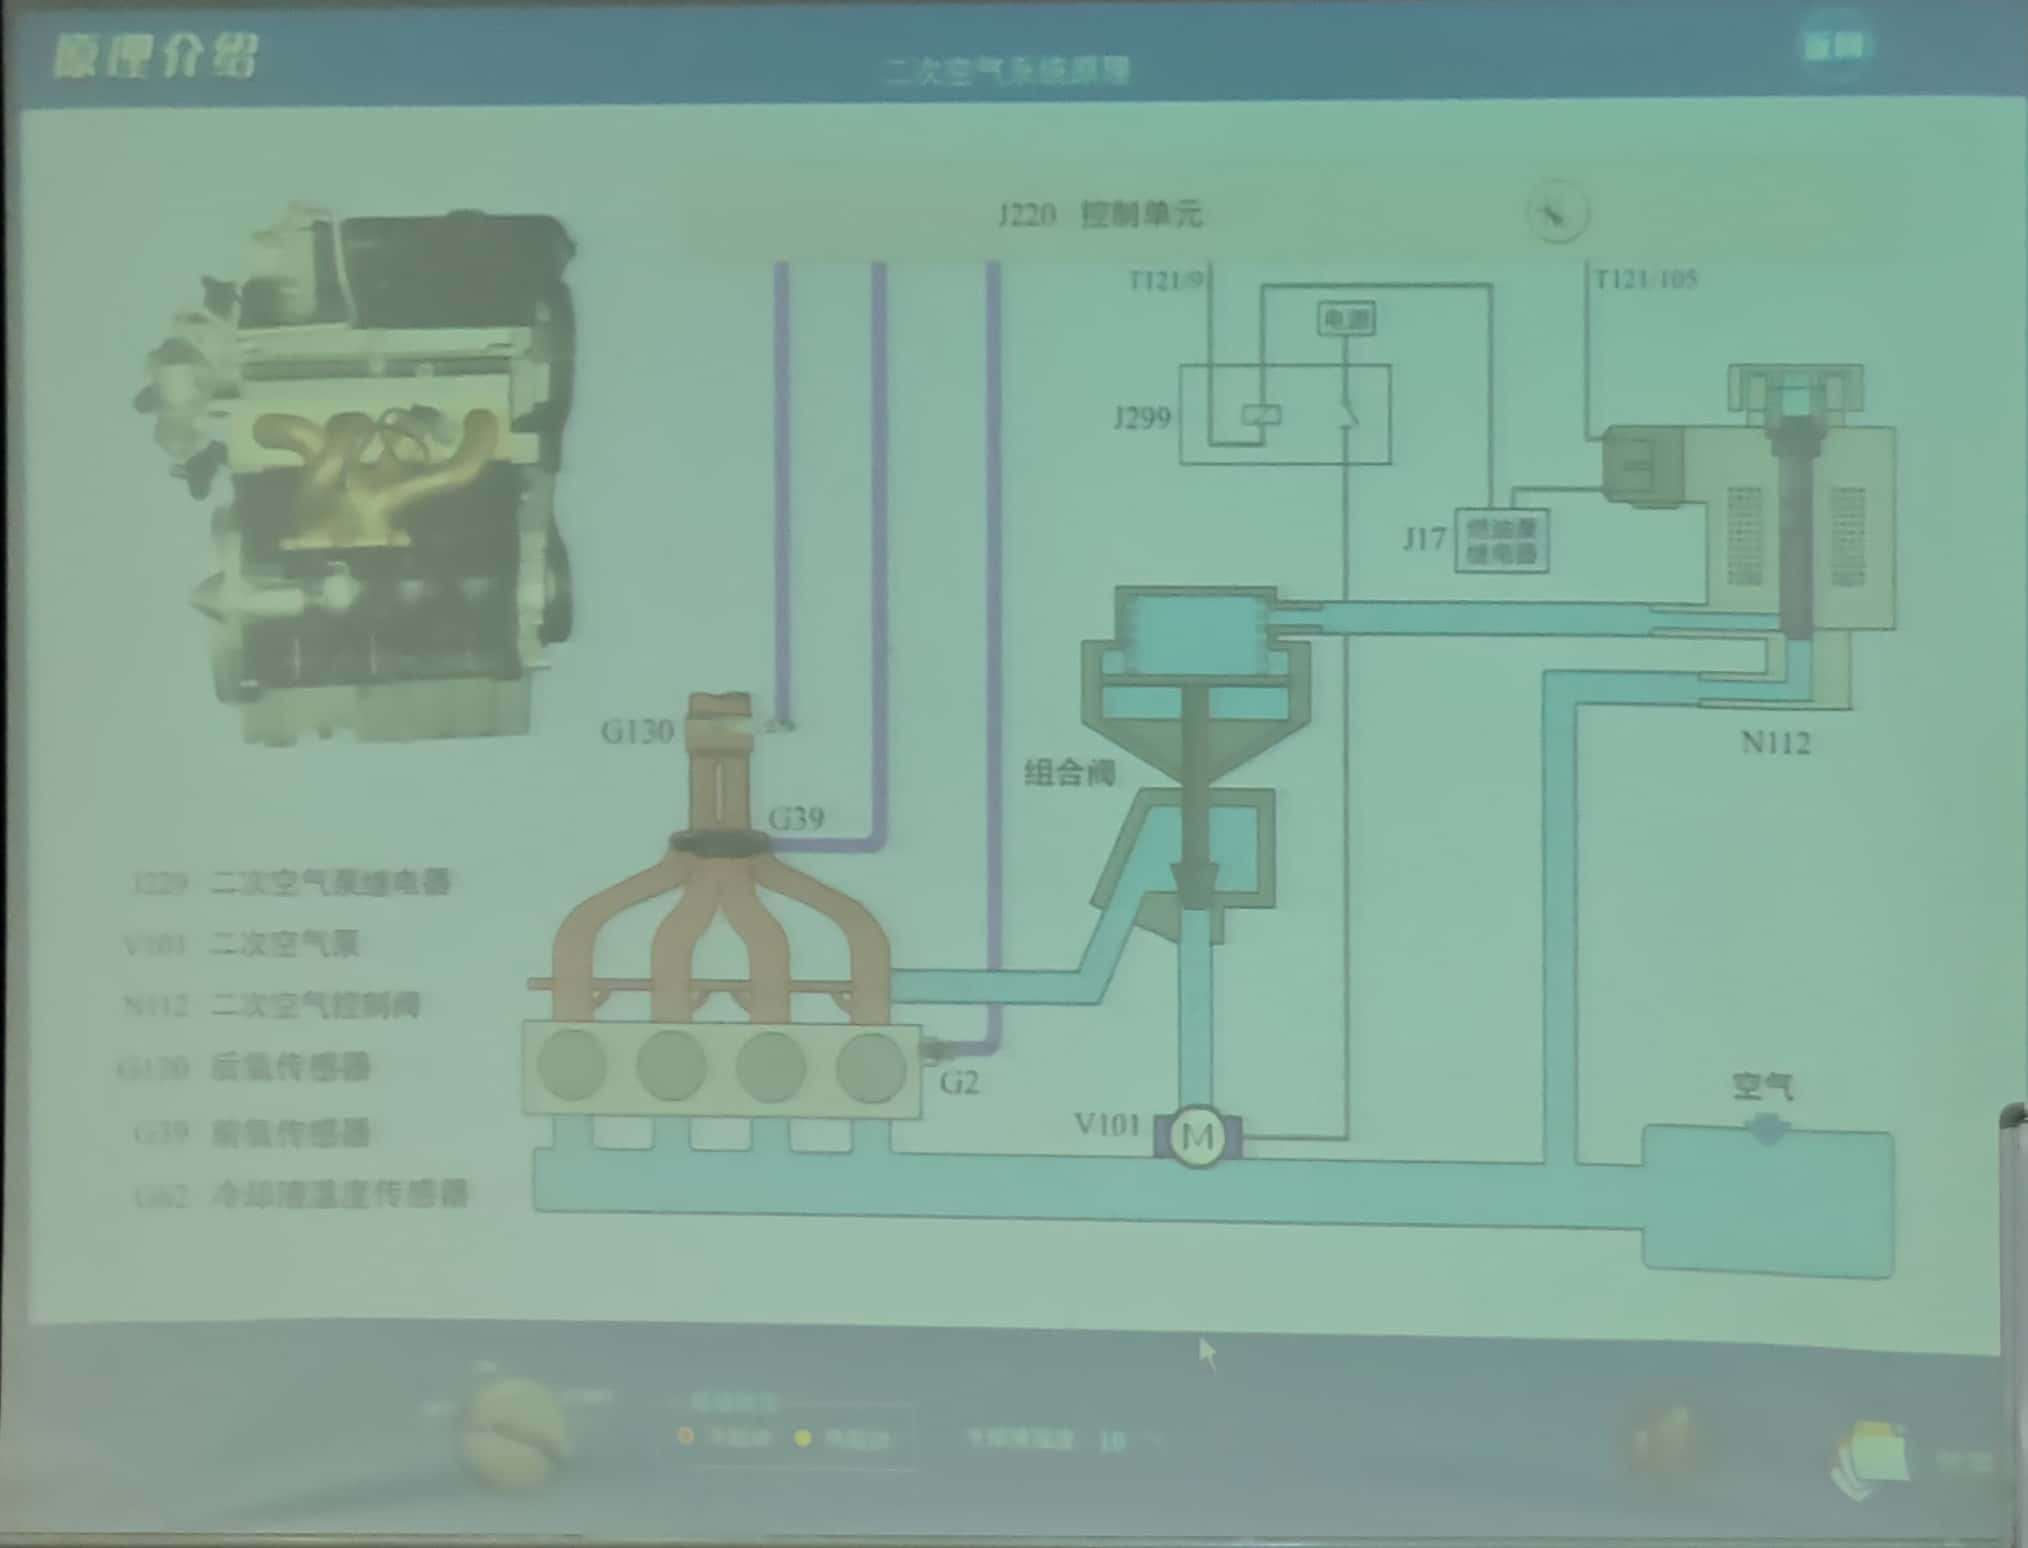
\includegraphics[width=0.3\textwidth]{secondary air}\label{secondary air}}
	\subfigure[排气再循环]{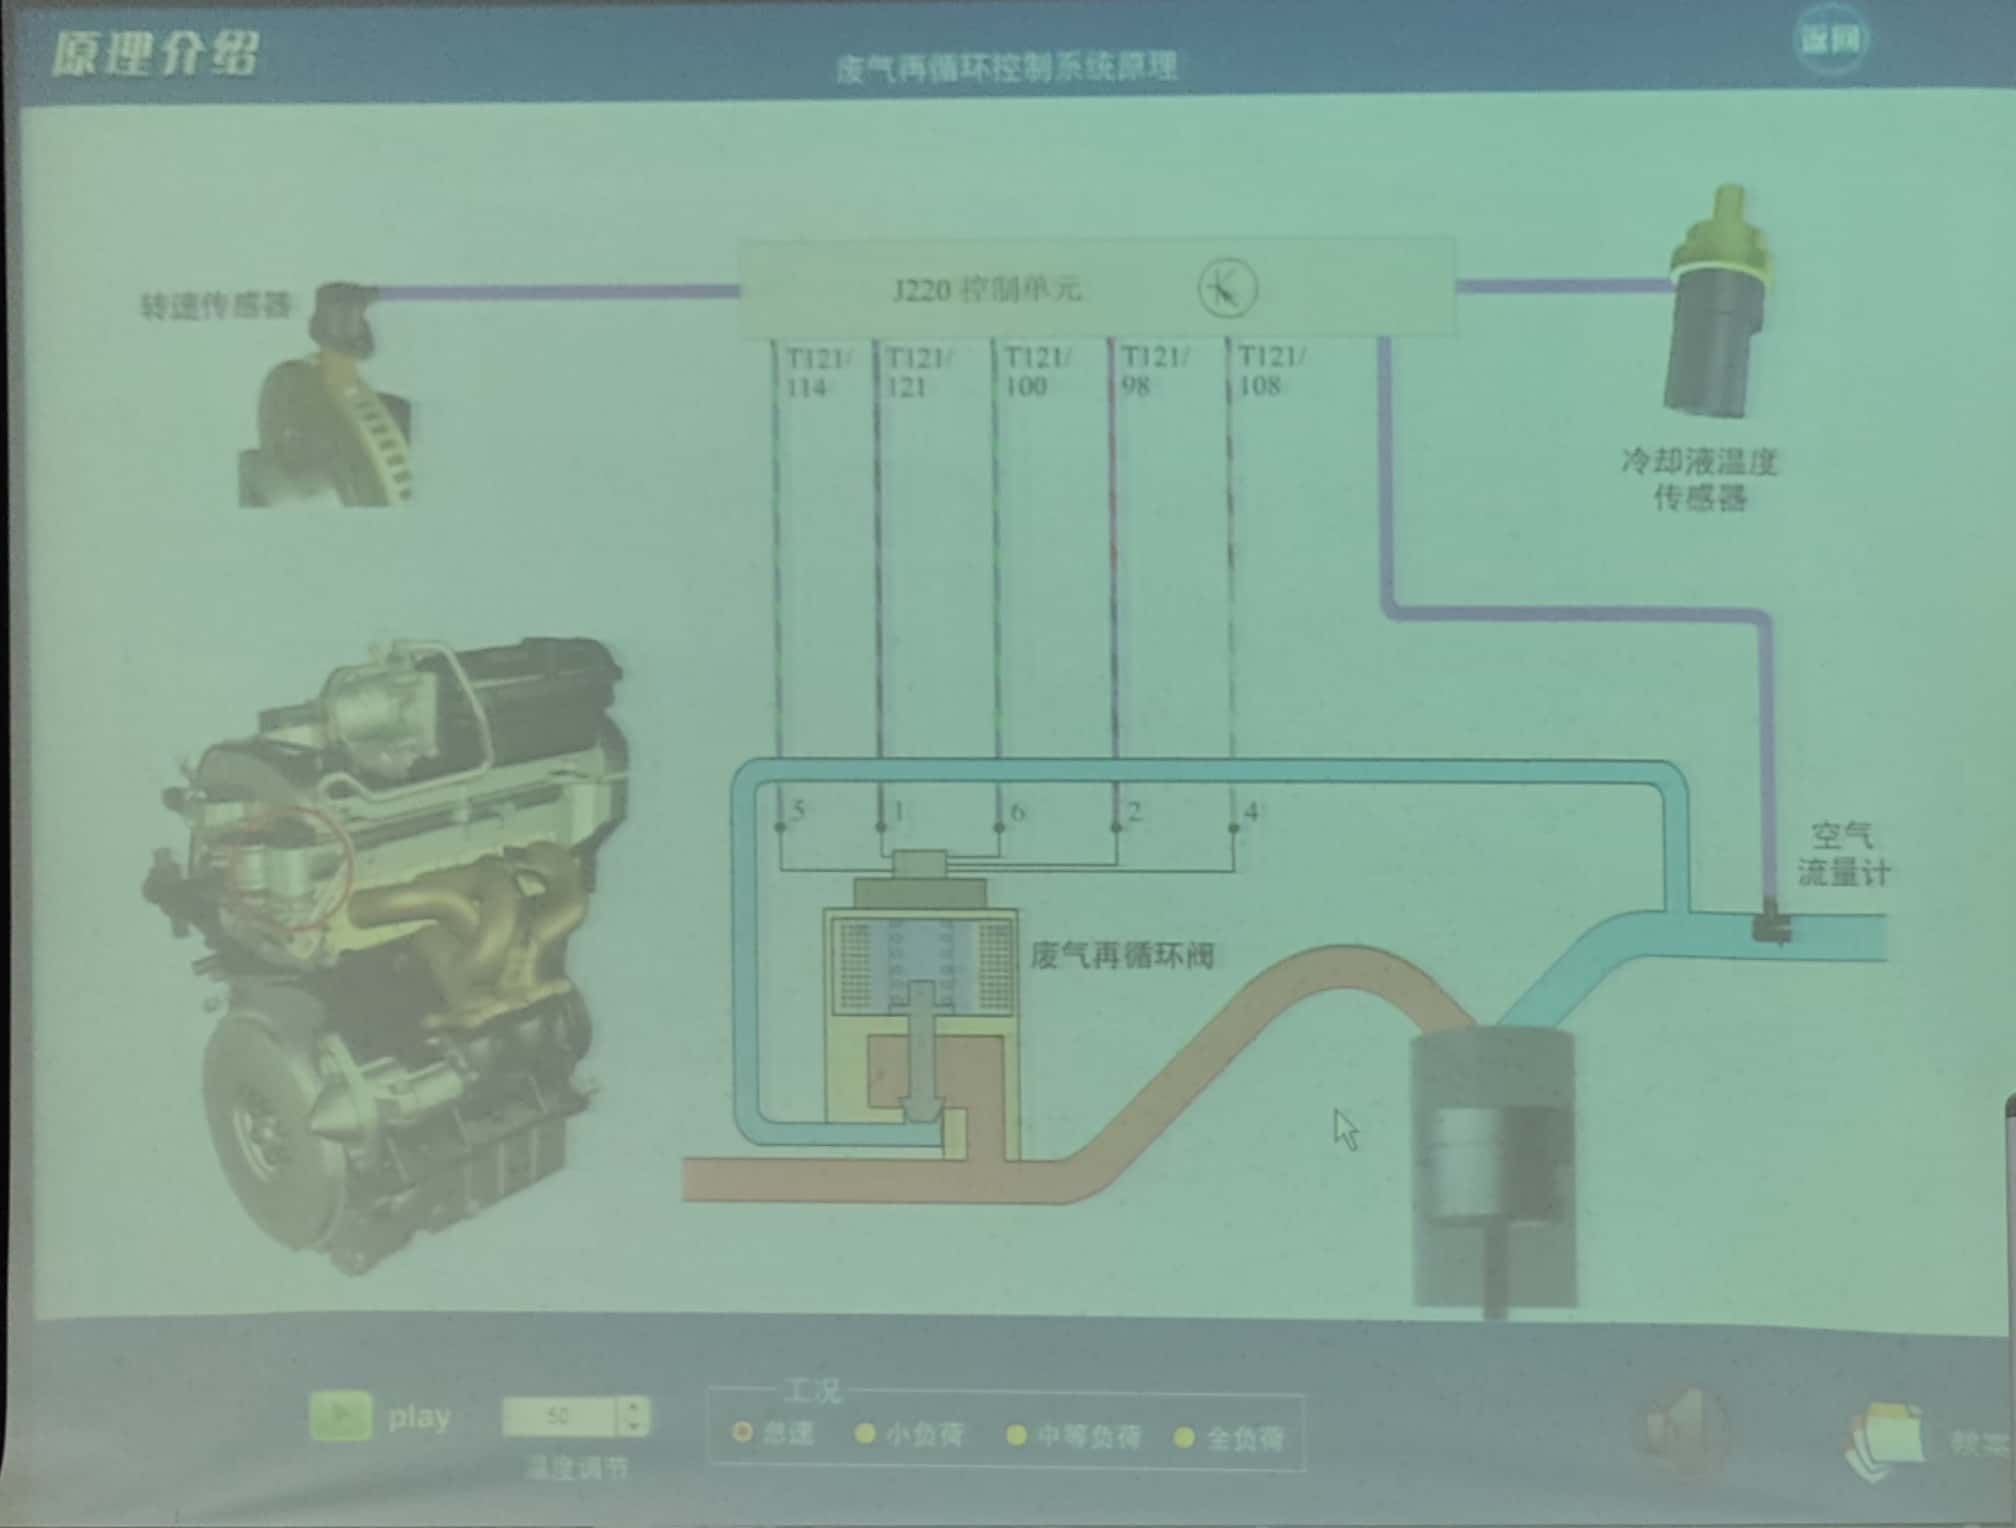
\includegraphics[width=0.3\textwidth]{EGR}\label{EGR}}
	\subfigure[废气涡轮增压]{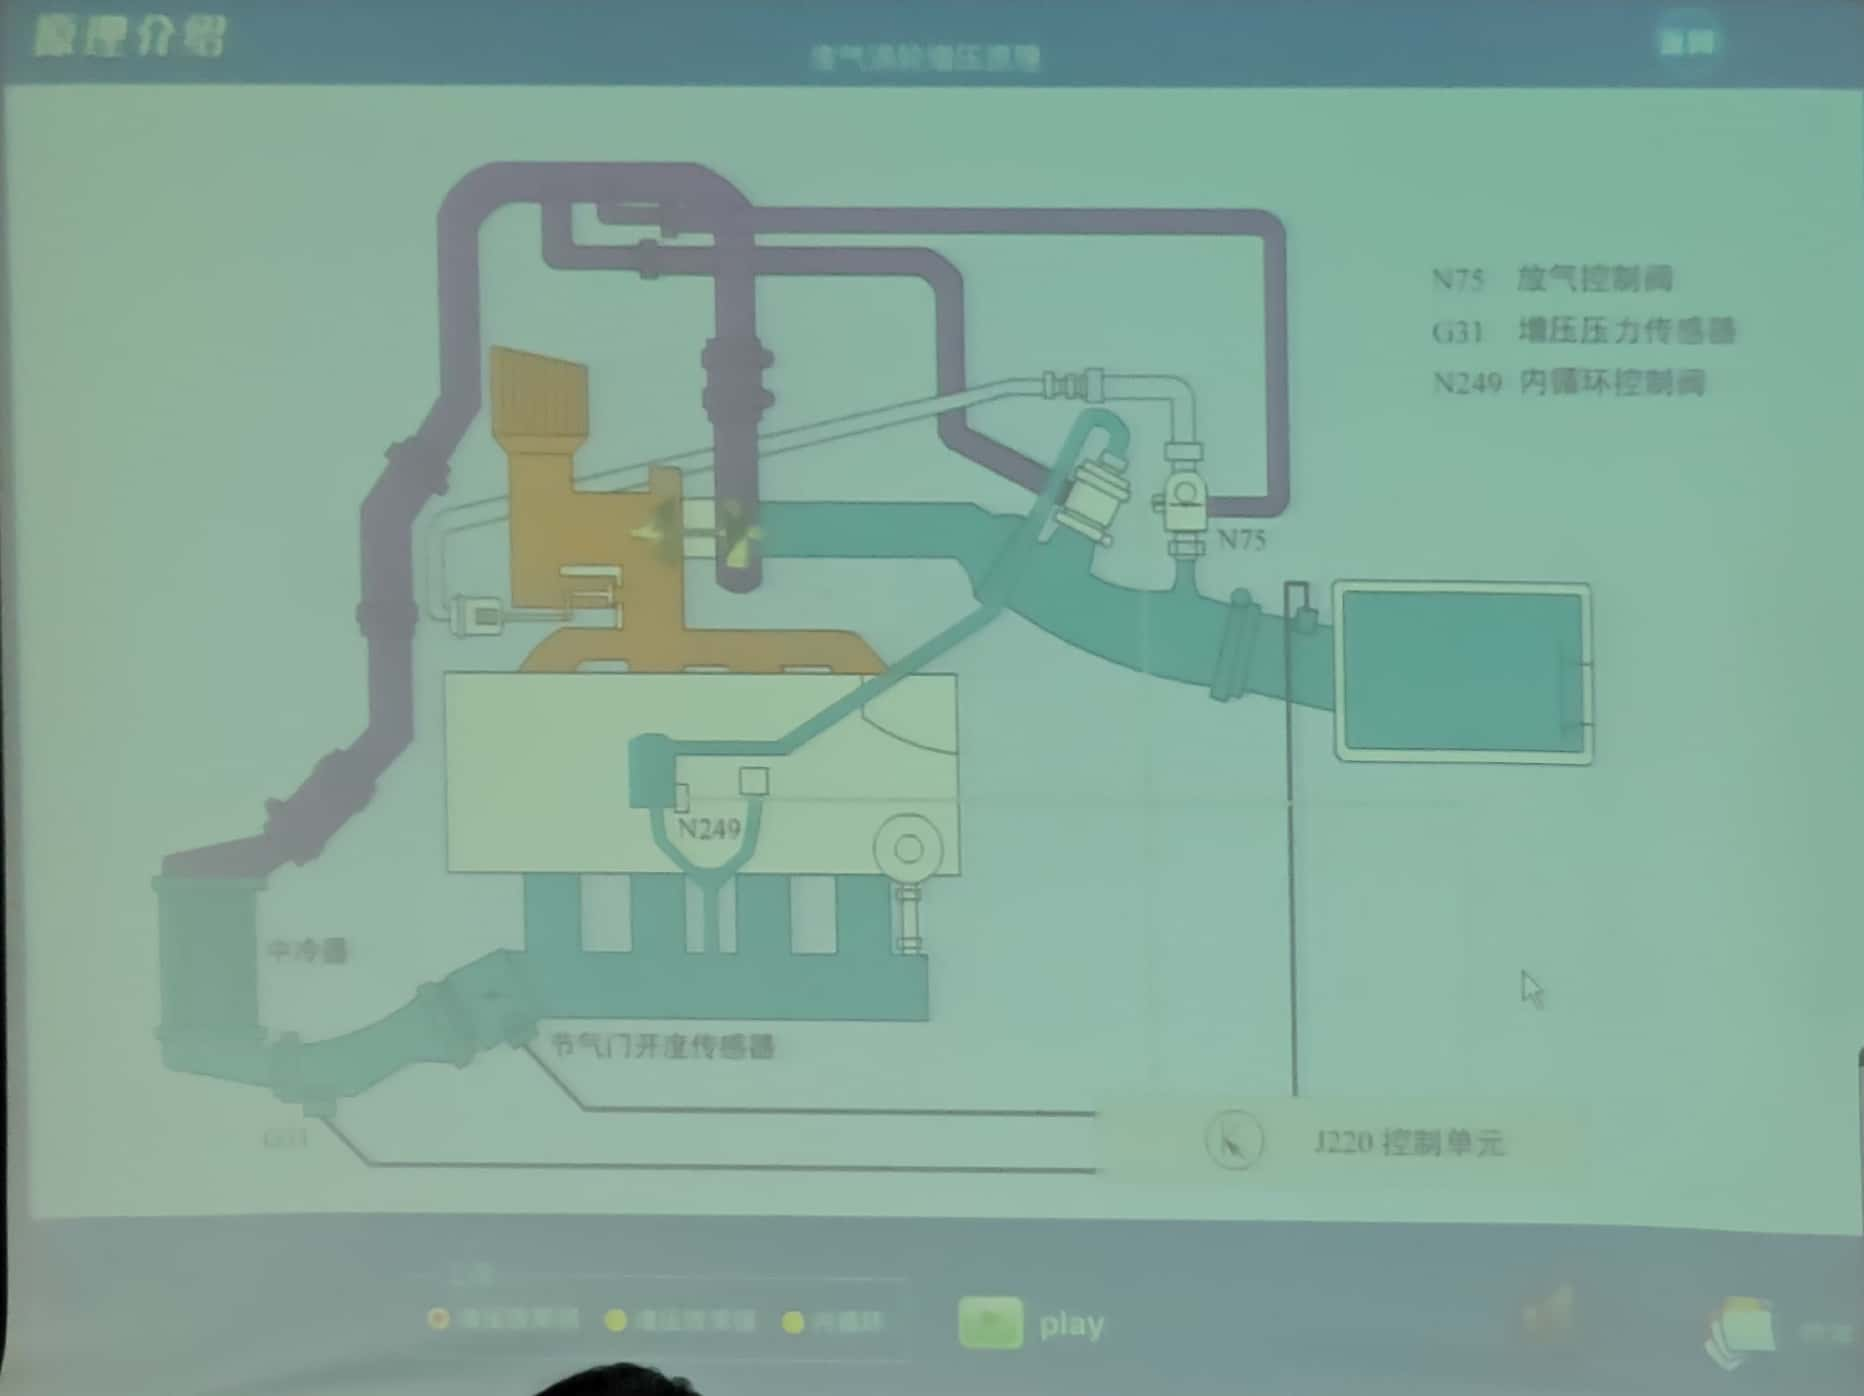
\includegraphics[width=0.3\textwidth]{turbocharging}\label{turbocharging}}
	\caption{发动机的控制系统中的部分执行器}
	\label{actuators}
\end{figure}

\subsection{请简述车身的主要功能及其实现方式。}

汽车车身是驾驶人的工作场所,也是装载乘客和货物的场所。

车身为驾驶员提供良好的操作条件,为乘员提供舒适的乘坐条件,并保证完好无损地运载货物且装卸方便。车身四周装有车窗,车身内外配备后视镜,部分新款汽车在车身周围还安装了多组传感器,驾驶员能清晰地感知车周环境。车内有仪表板,座椅、方向盘、后视镜等附件的位置可调,方便驾驶员掌握车辆情况。对乘员来说,发动机舱盖上有隔音棉(\cref{sound insulation cotton}),车门和车顶中空除方便车窗、天窗开闭外也可提升隔音、隔热效果,炽热的排气管与车身底部间覆盖隔热材料(\cref{insulation}),可开合的门四周覆盖胶条密封以隔音、防水,舒适的座椅起部分隔振功能,这些措施都让乘员与外界较恶劣的环境隔绝,提升舒适性。车身上开门位置合理,乘员能方便上下车,货物能方便装卸。对于货车来说车身上设有货物固定装置,避免运输时货物滑移、倾倒。

\begin{figure}[htbp]
	\centering
	\begin{minipage}[b]{0.7\textwidth}
		\centering
		
\includegraphics[width=\textwidth]{sound insulation cotton}
		\caption{隔音棉}
		\label{sound insulation cotton}
	\end{minipage}
	\begin{minipage}[b]{0.25\textwidth}
		\centering
		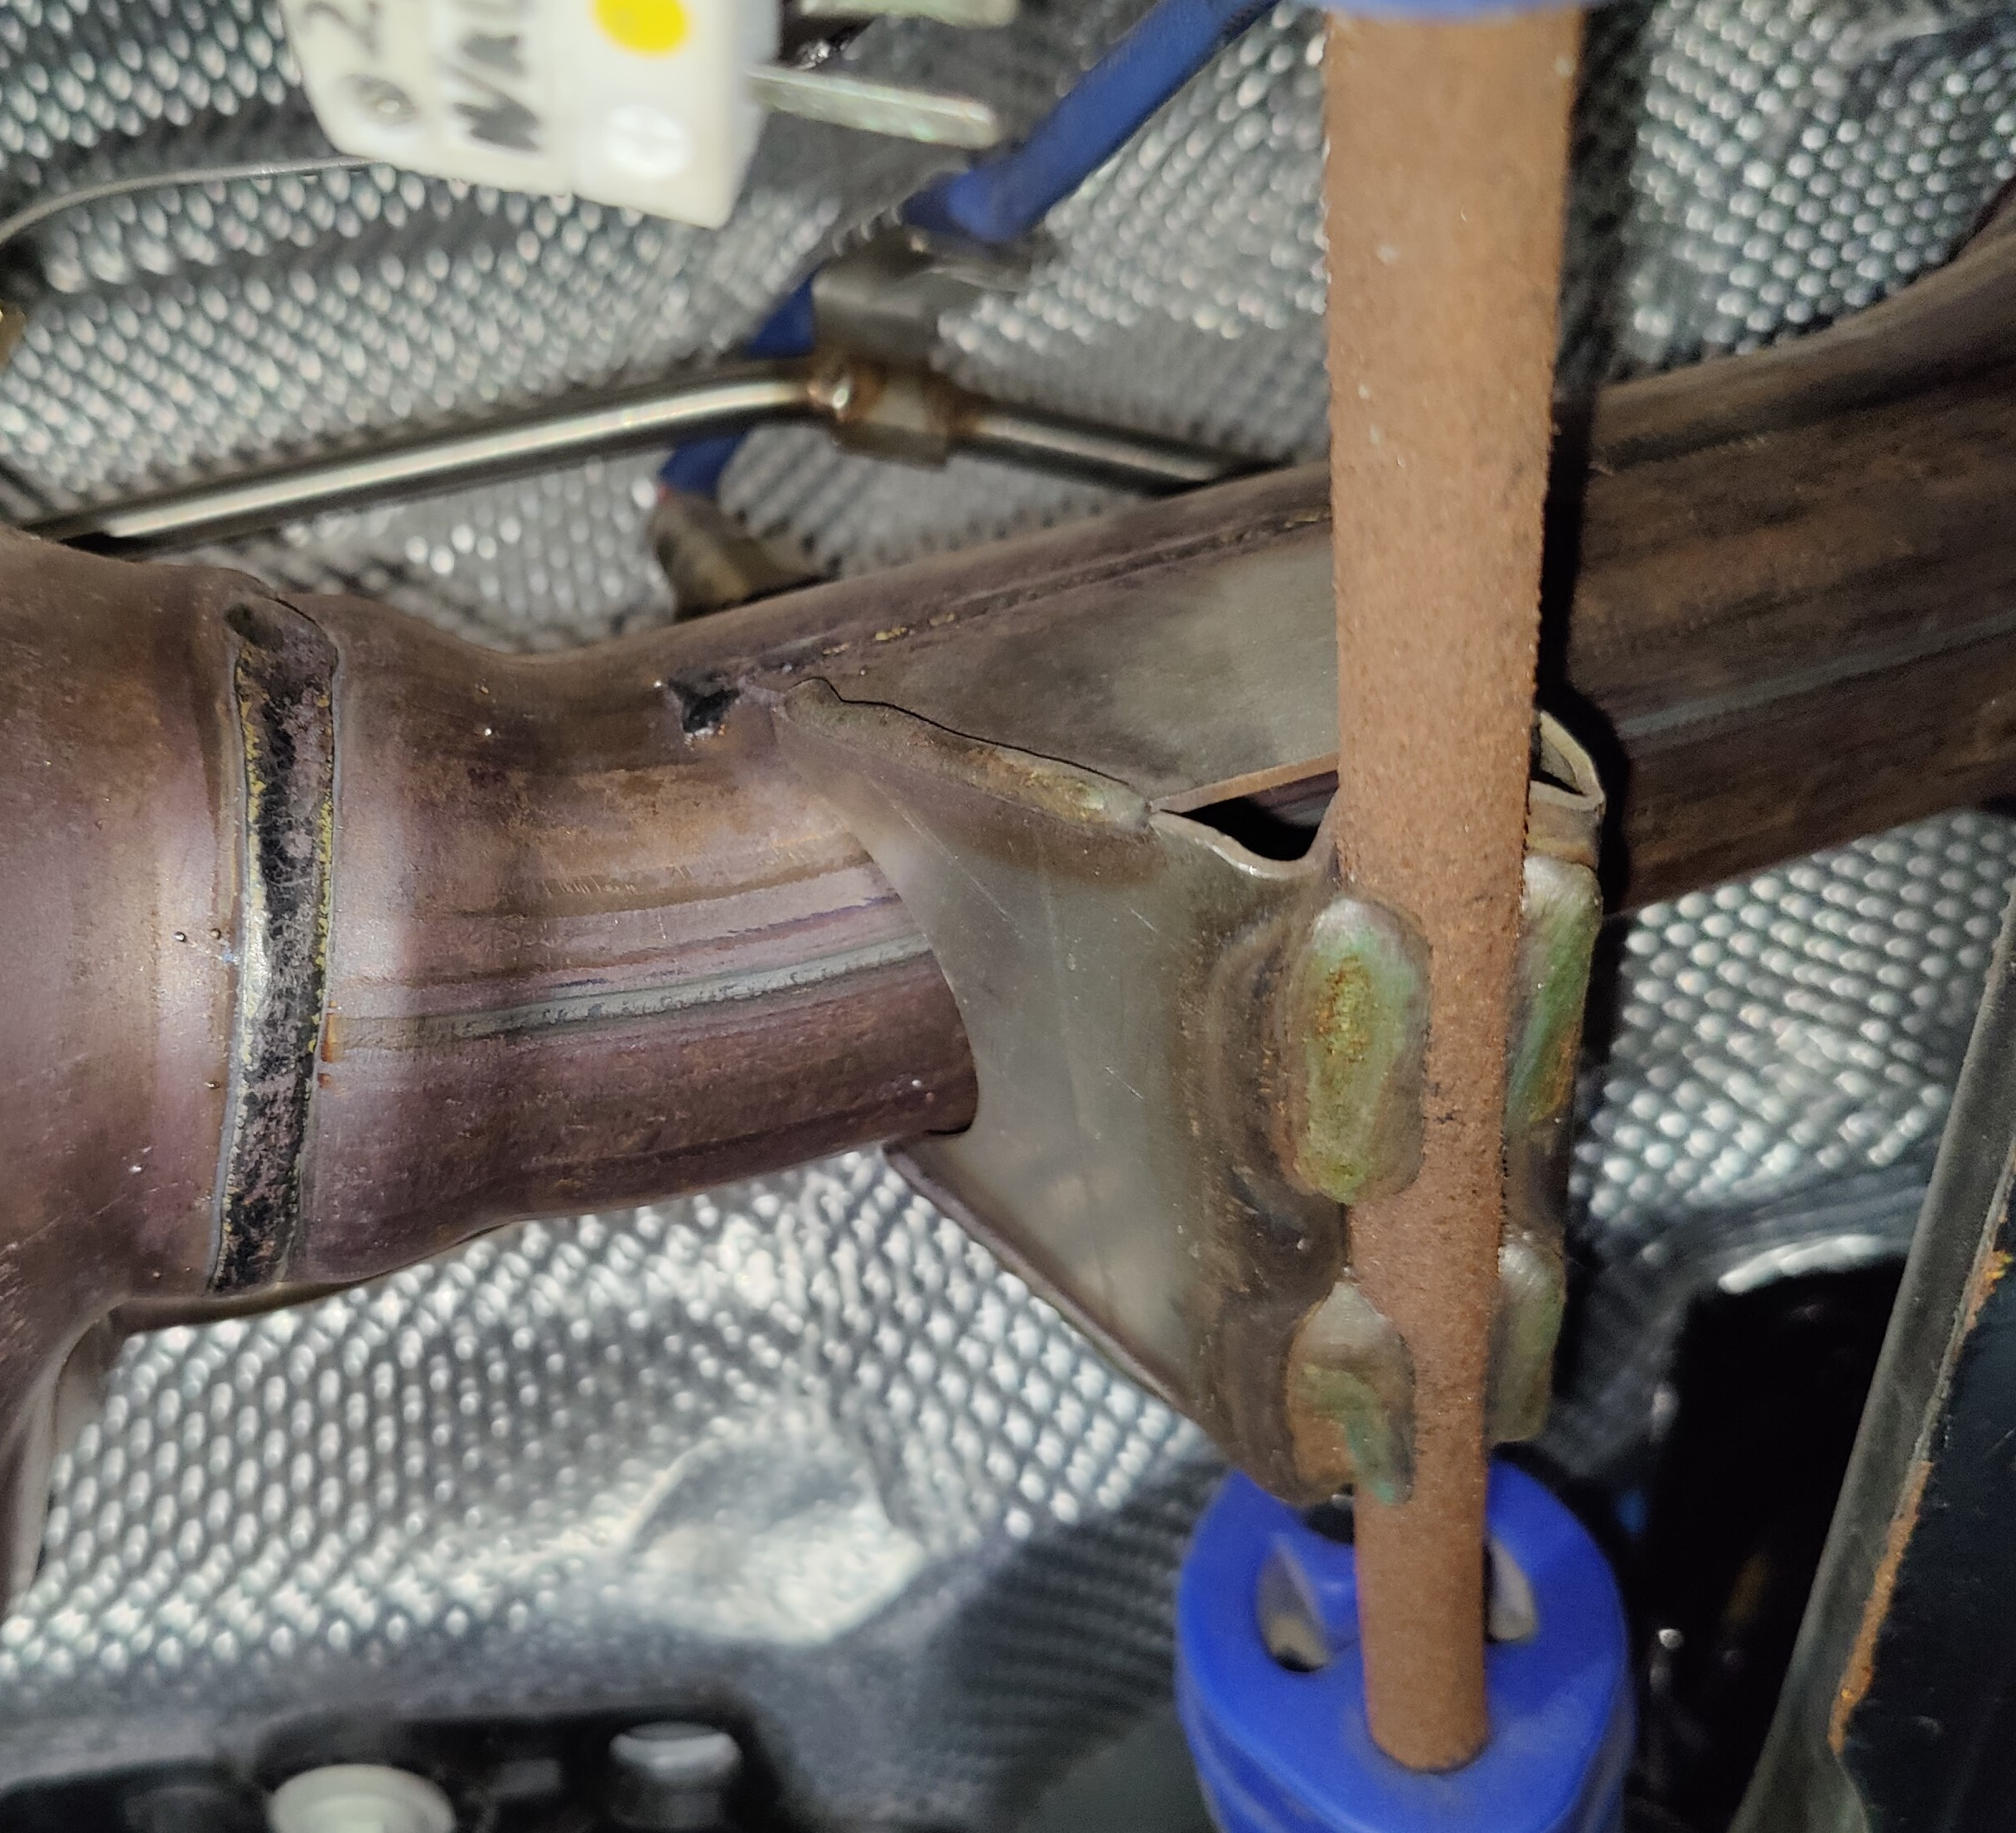
\includegraphics[width=\textwidth]{insulation}
		\caption{隔热材料}
		\label{insulation}
	\end{minipage}
\end{figure}

碰撞安全性是车身结构和设备设计时需要重点考虑的。\cref{BIW}为白车身的一部分,注意到涂有红色油漆的钢梁均由高强钢制成,起防撞梁的作用。保险杠安装梁与车身本体间有缓冲装置,部分高配车型上这里会安装弹性元件和阻尼器,缓和正碰时冲击。车门内部也有高强度的防撞梁,增强侧碰安全性。车上装有多个安全气囊,和安全带一起避免碰撞时乘员重要部位直接与硬物接触,保护乘员。现在对行人保护日趋重视,车身上通过吸能保险杠、软性的引擎盖材料、大灯及附件无锐角等措施保护低速碰撞时行人的安全。

\begin{figure}[htbp]
	\centering
	\begin{minipage}[b]{0.6\textwidth}
		\centering
		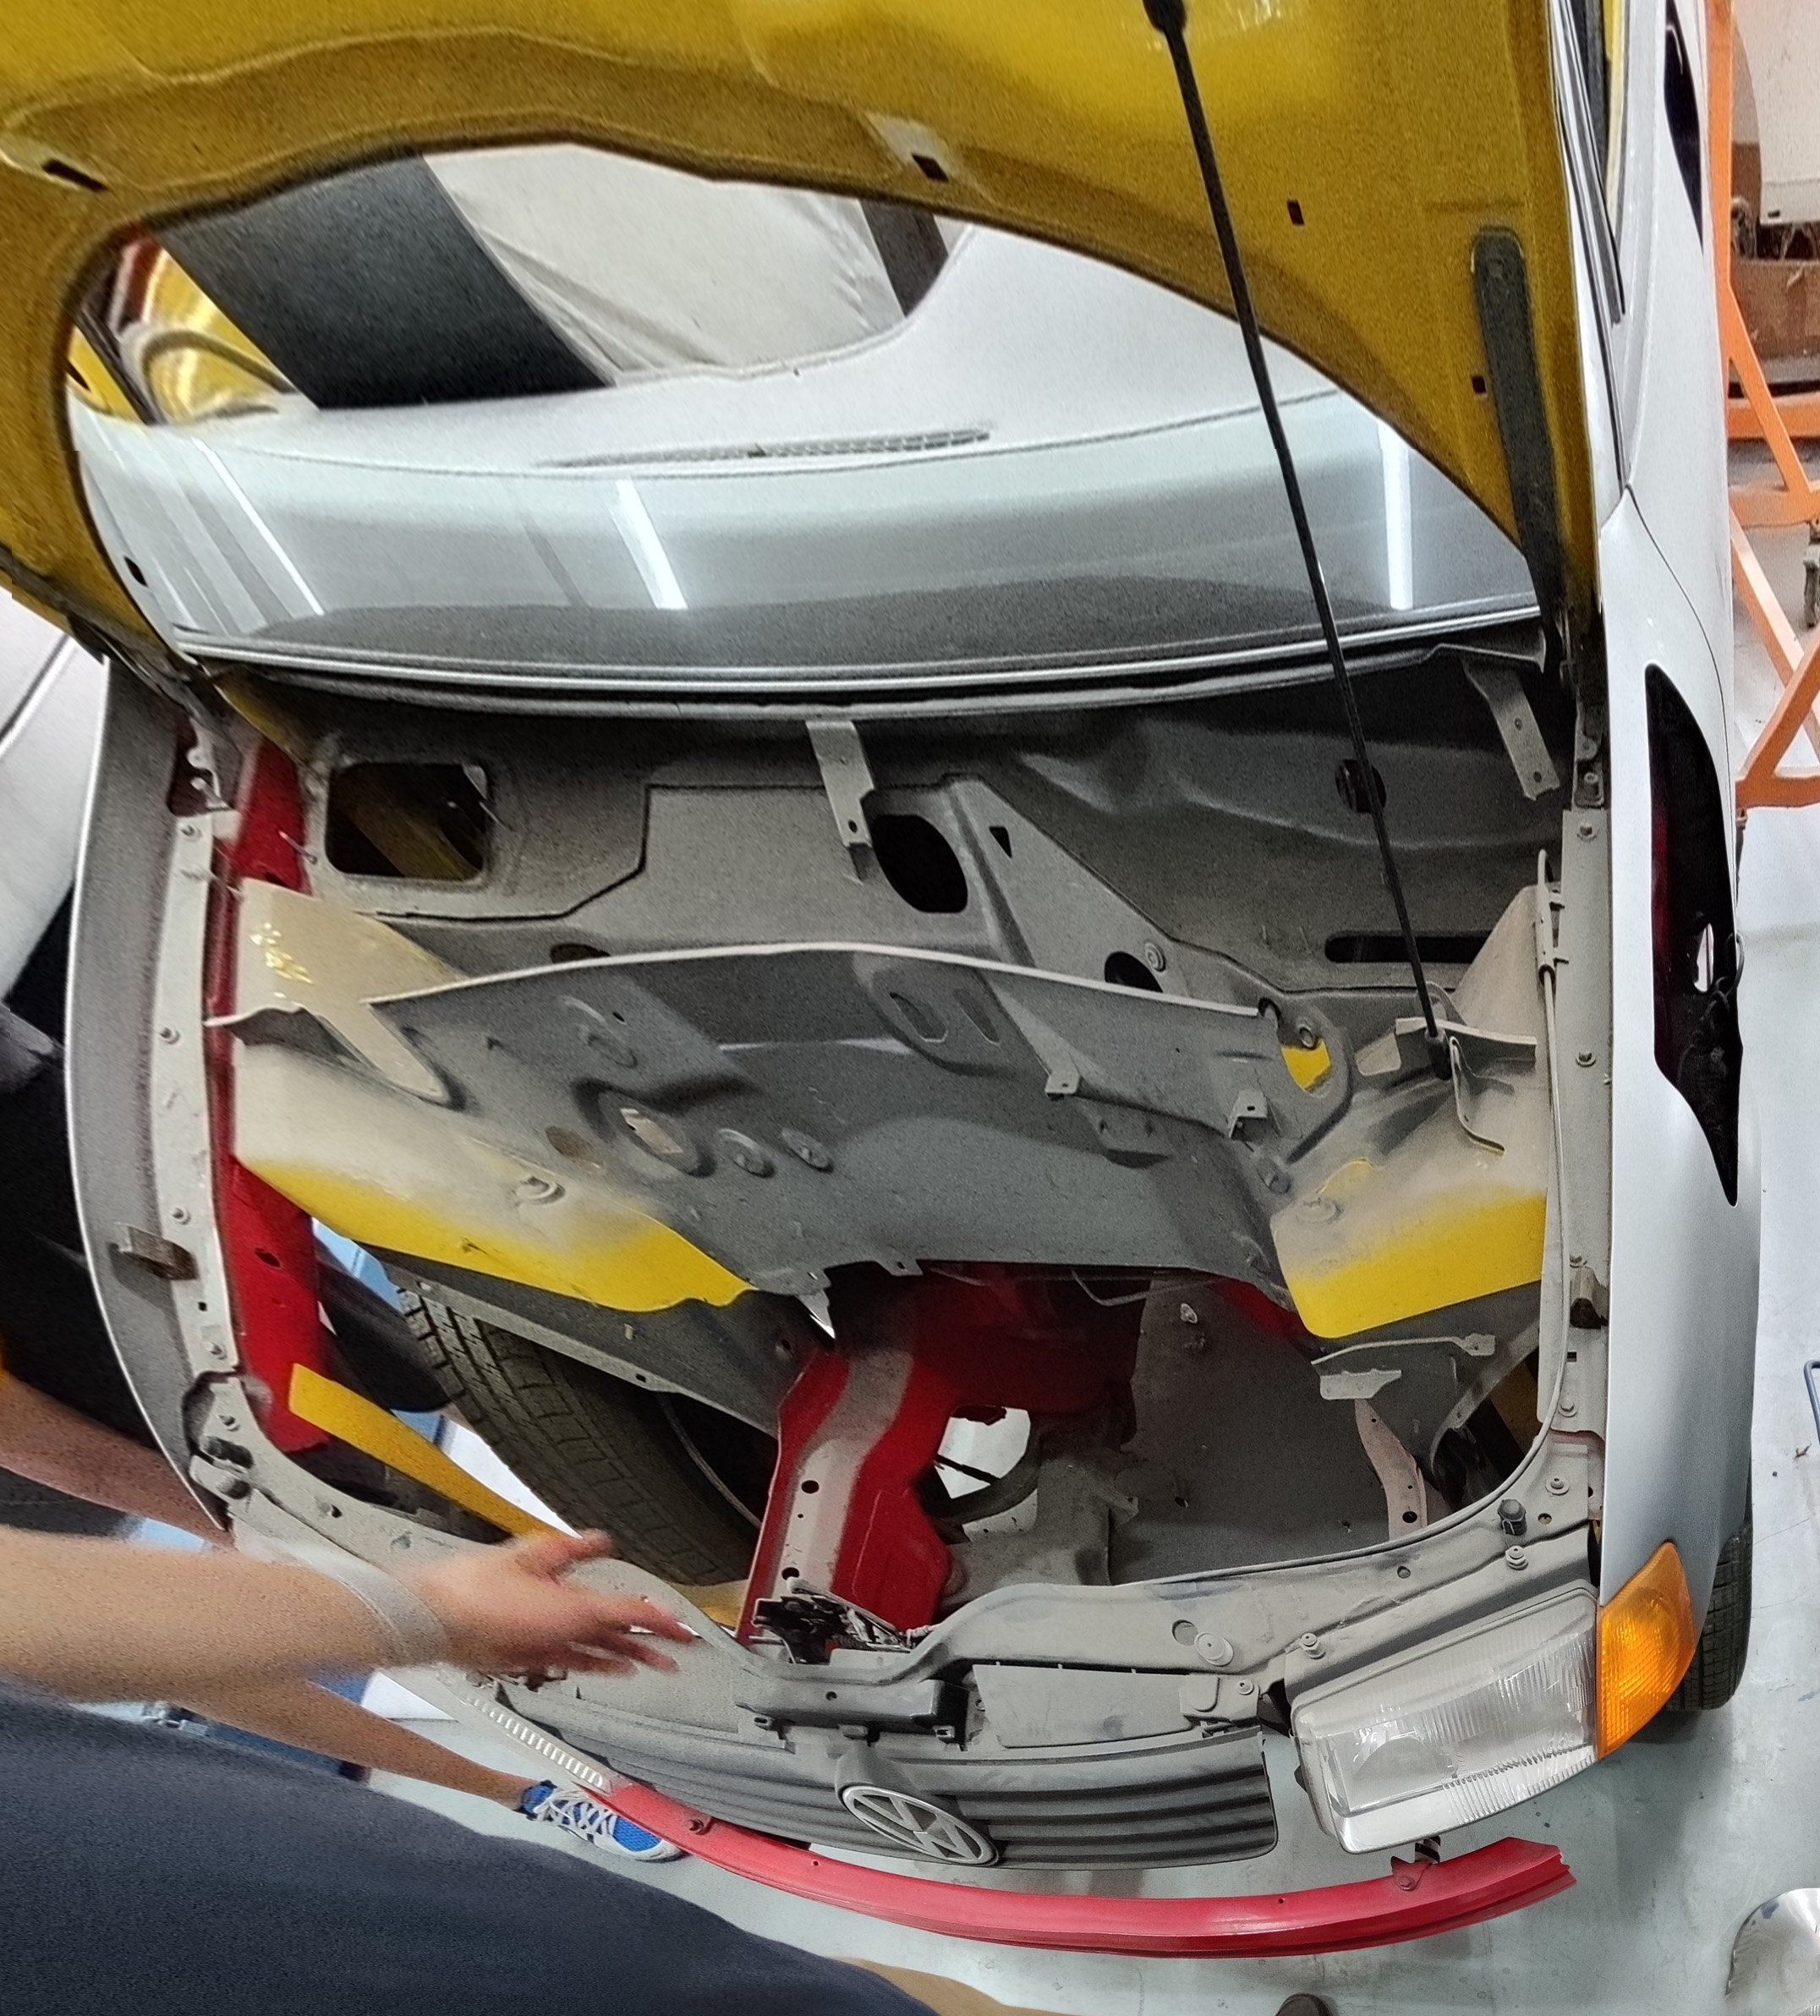
\includegraphics[width=\textwidth]{BIW}
		\caption{白车身}
		\label{BIW}
	\end{minipage}
\end{figure}

车身外形的设计要考虑空气动力学特性,以便汽车行驶时能有效引导周围的气流,提高汽车动力性和行驶稳定性,并改善发动机舱冷却条件和车内通风。注意到展示的领克02上发动机底板已被拆下(\cref{engine compartment bottom}),这能让我们方便地看到油底壳等发动机部件,但在车辆行驶过程中会带来较大的风阻增加,故实际车辆上发动机舱底部有一平板用于引导气流,如\cref{engine compartment with floor}所示,该底板还可兼起保护油底壳免受异物碰撞的作用。对于一般的发动机前置车型,车身头部开有进气孔,还可布置冷排,供发动机进气、冷却。现在的车身越来越向流线型发展,这主要也是出于降阻的考虑。

\begin{figure}[htbp]
	\centering
	\begin{minipage}[b]{0.4\textwidth}
		\centering
		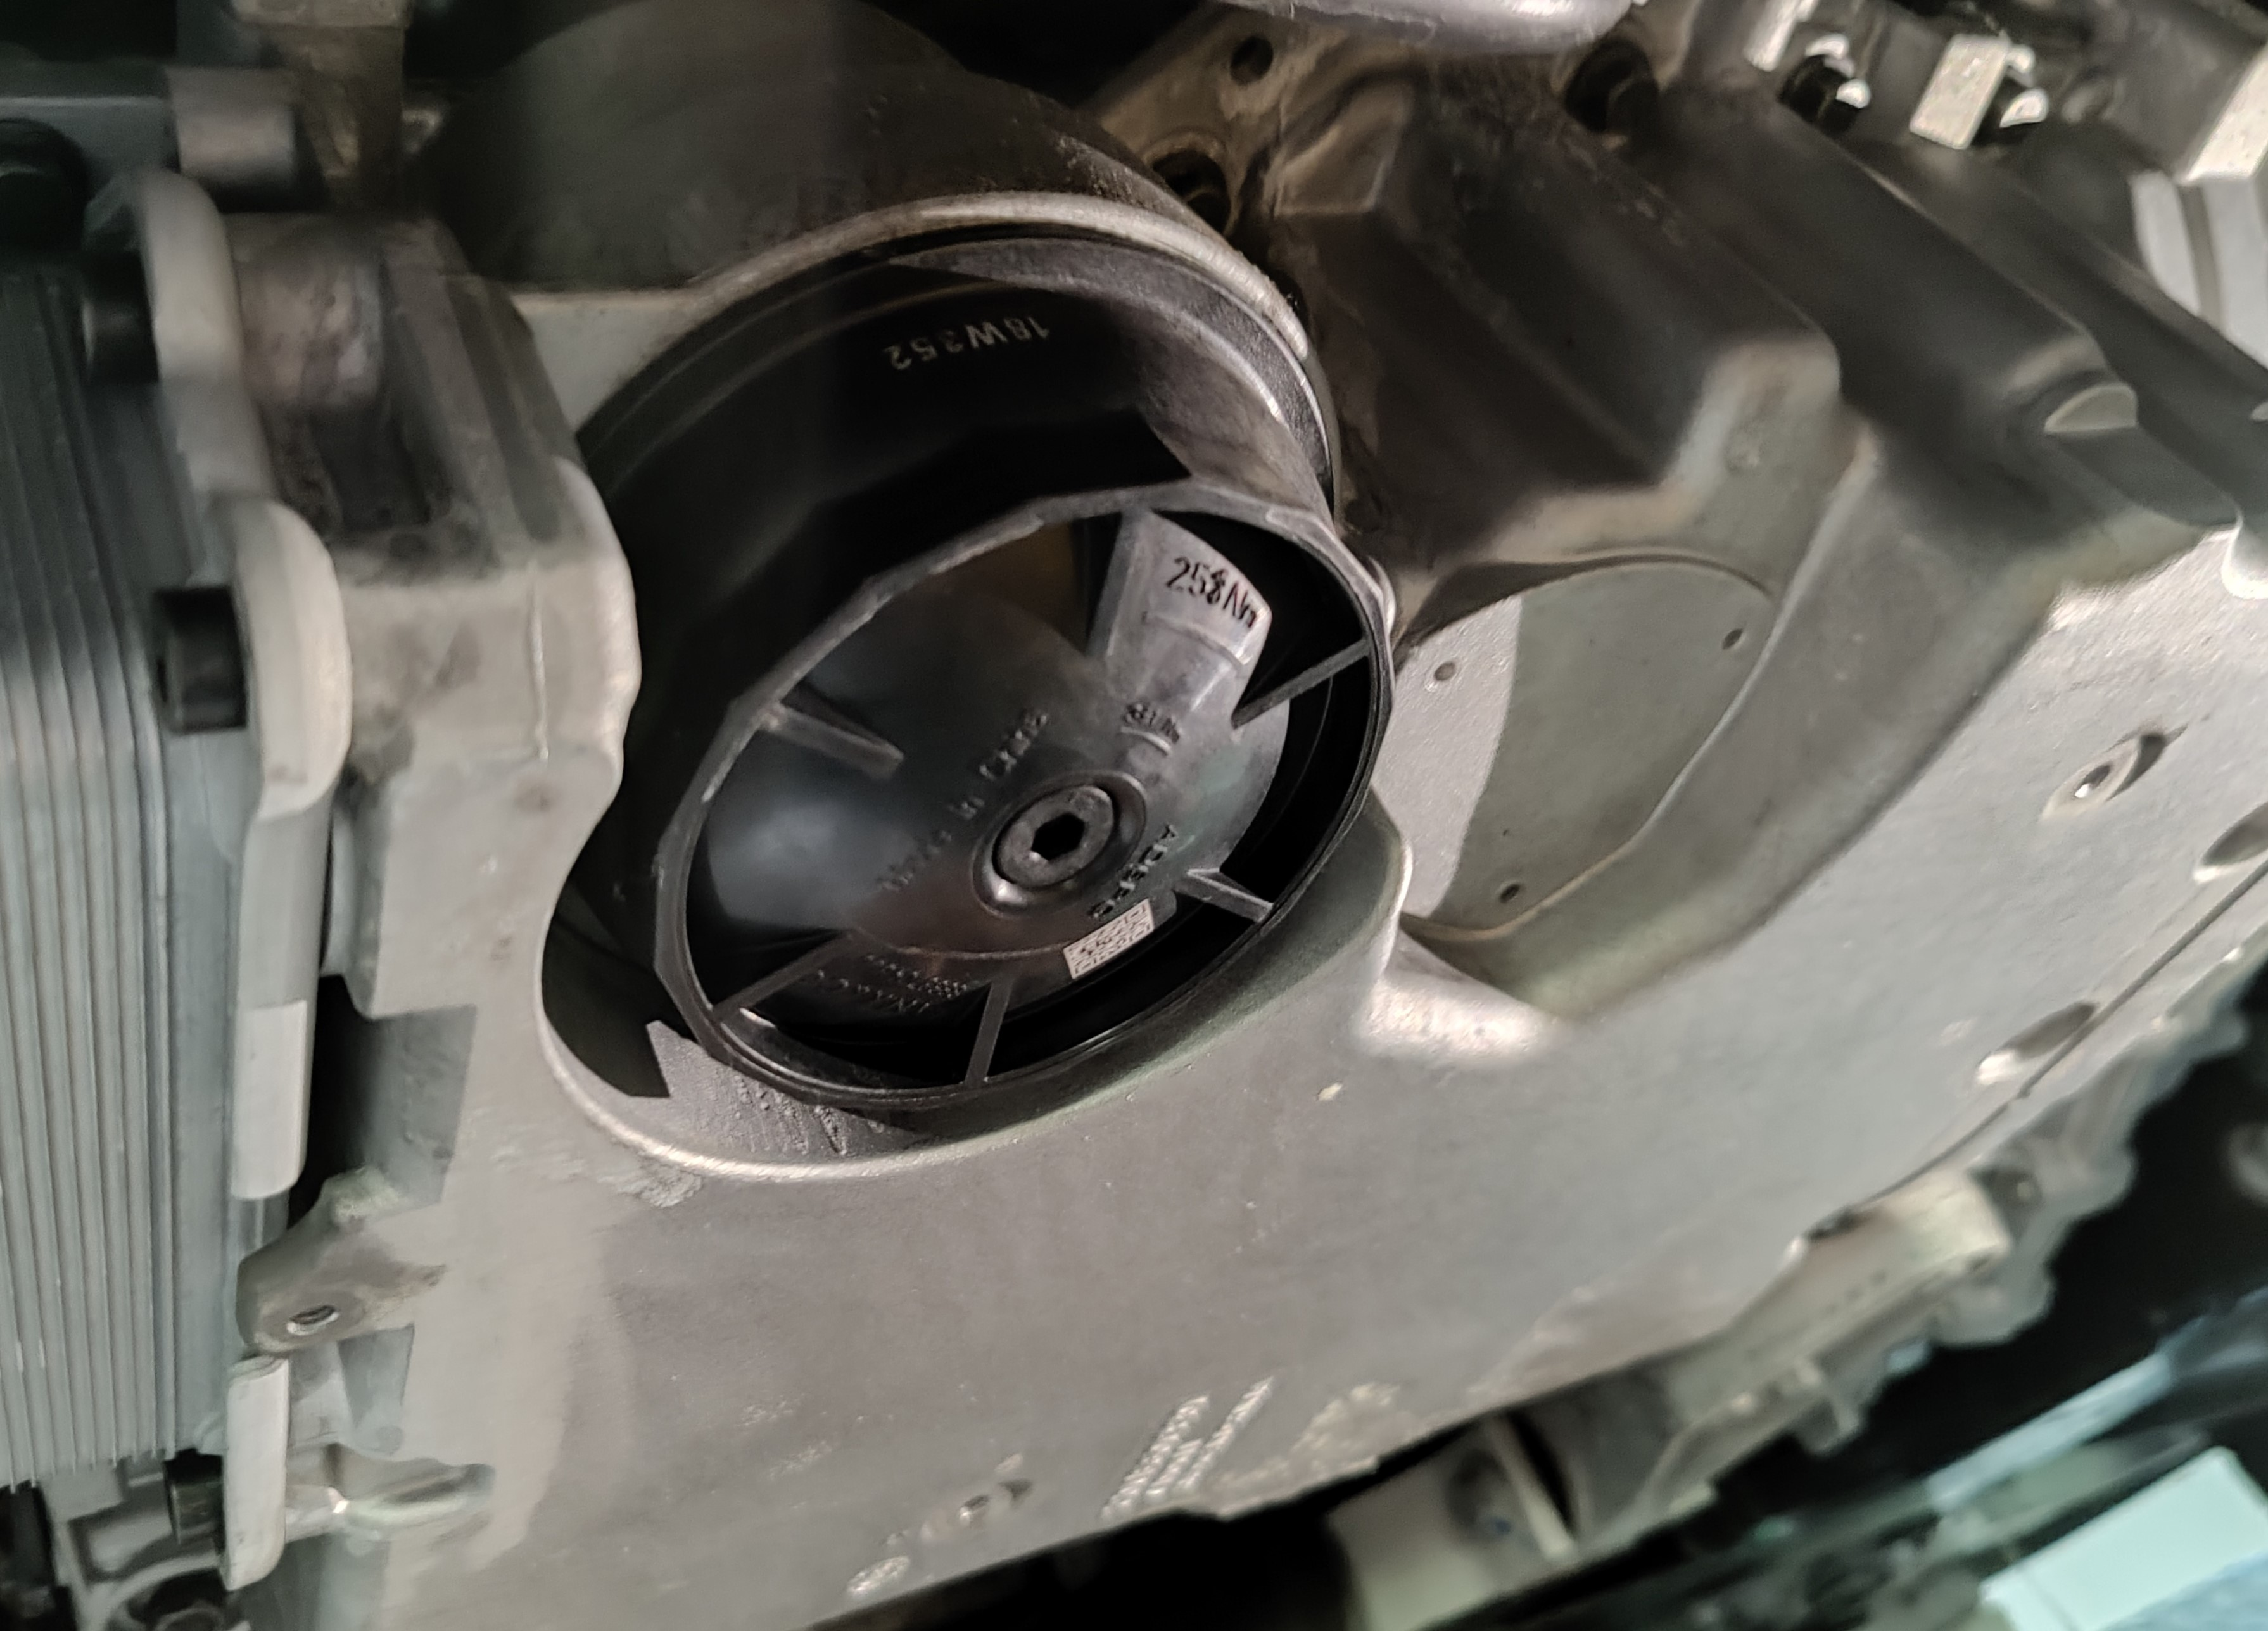
\includegraphics[width=\textwidth]{engine compartment bottom}
		\caption{发动机舱底部}
		\label{engine compartment bottom}
	\end{minipage}
	\begin{minipage}[b]{0.5\textwidth}
		\centering
		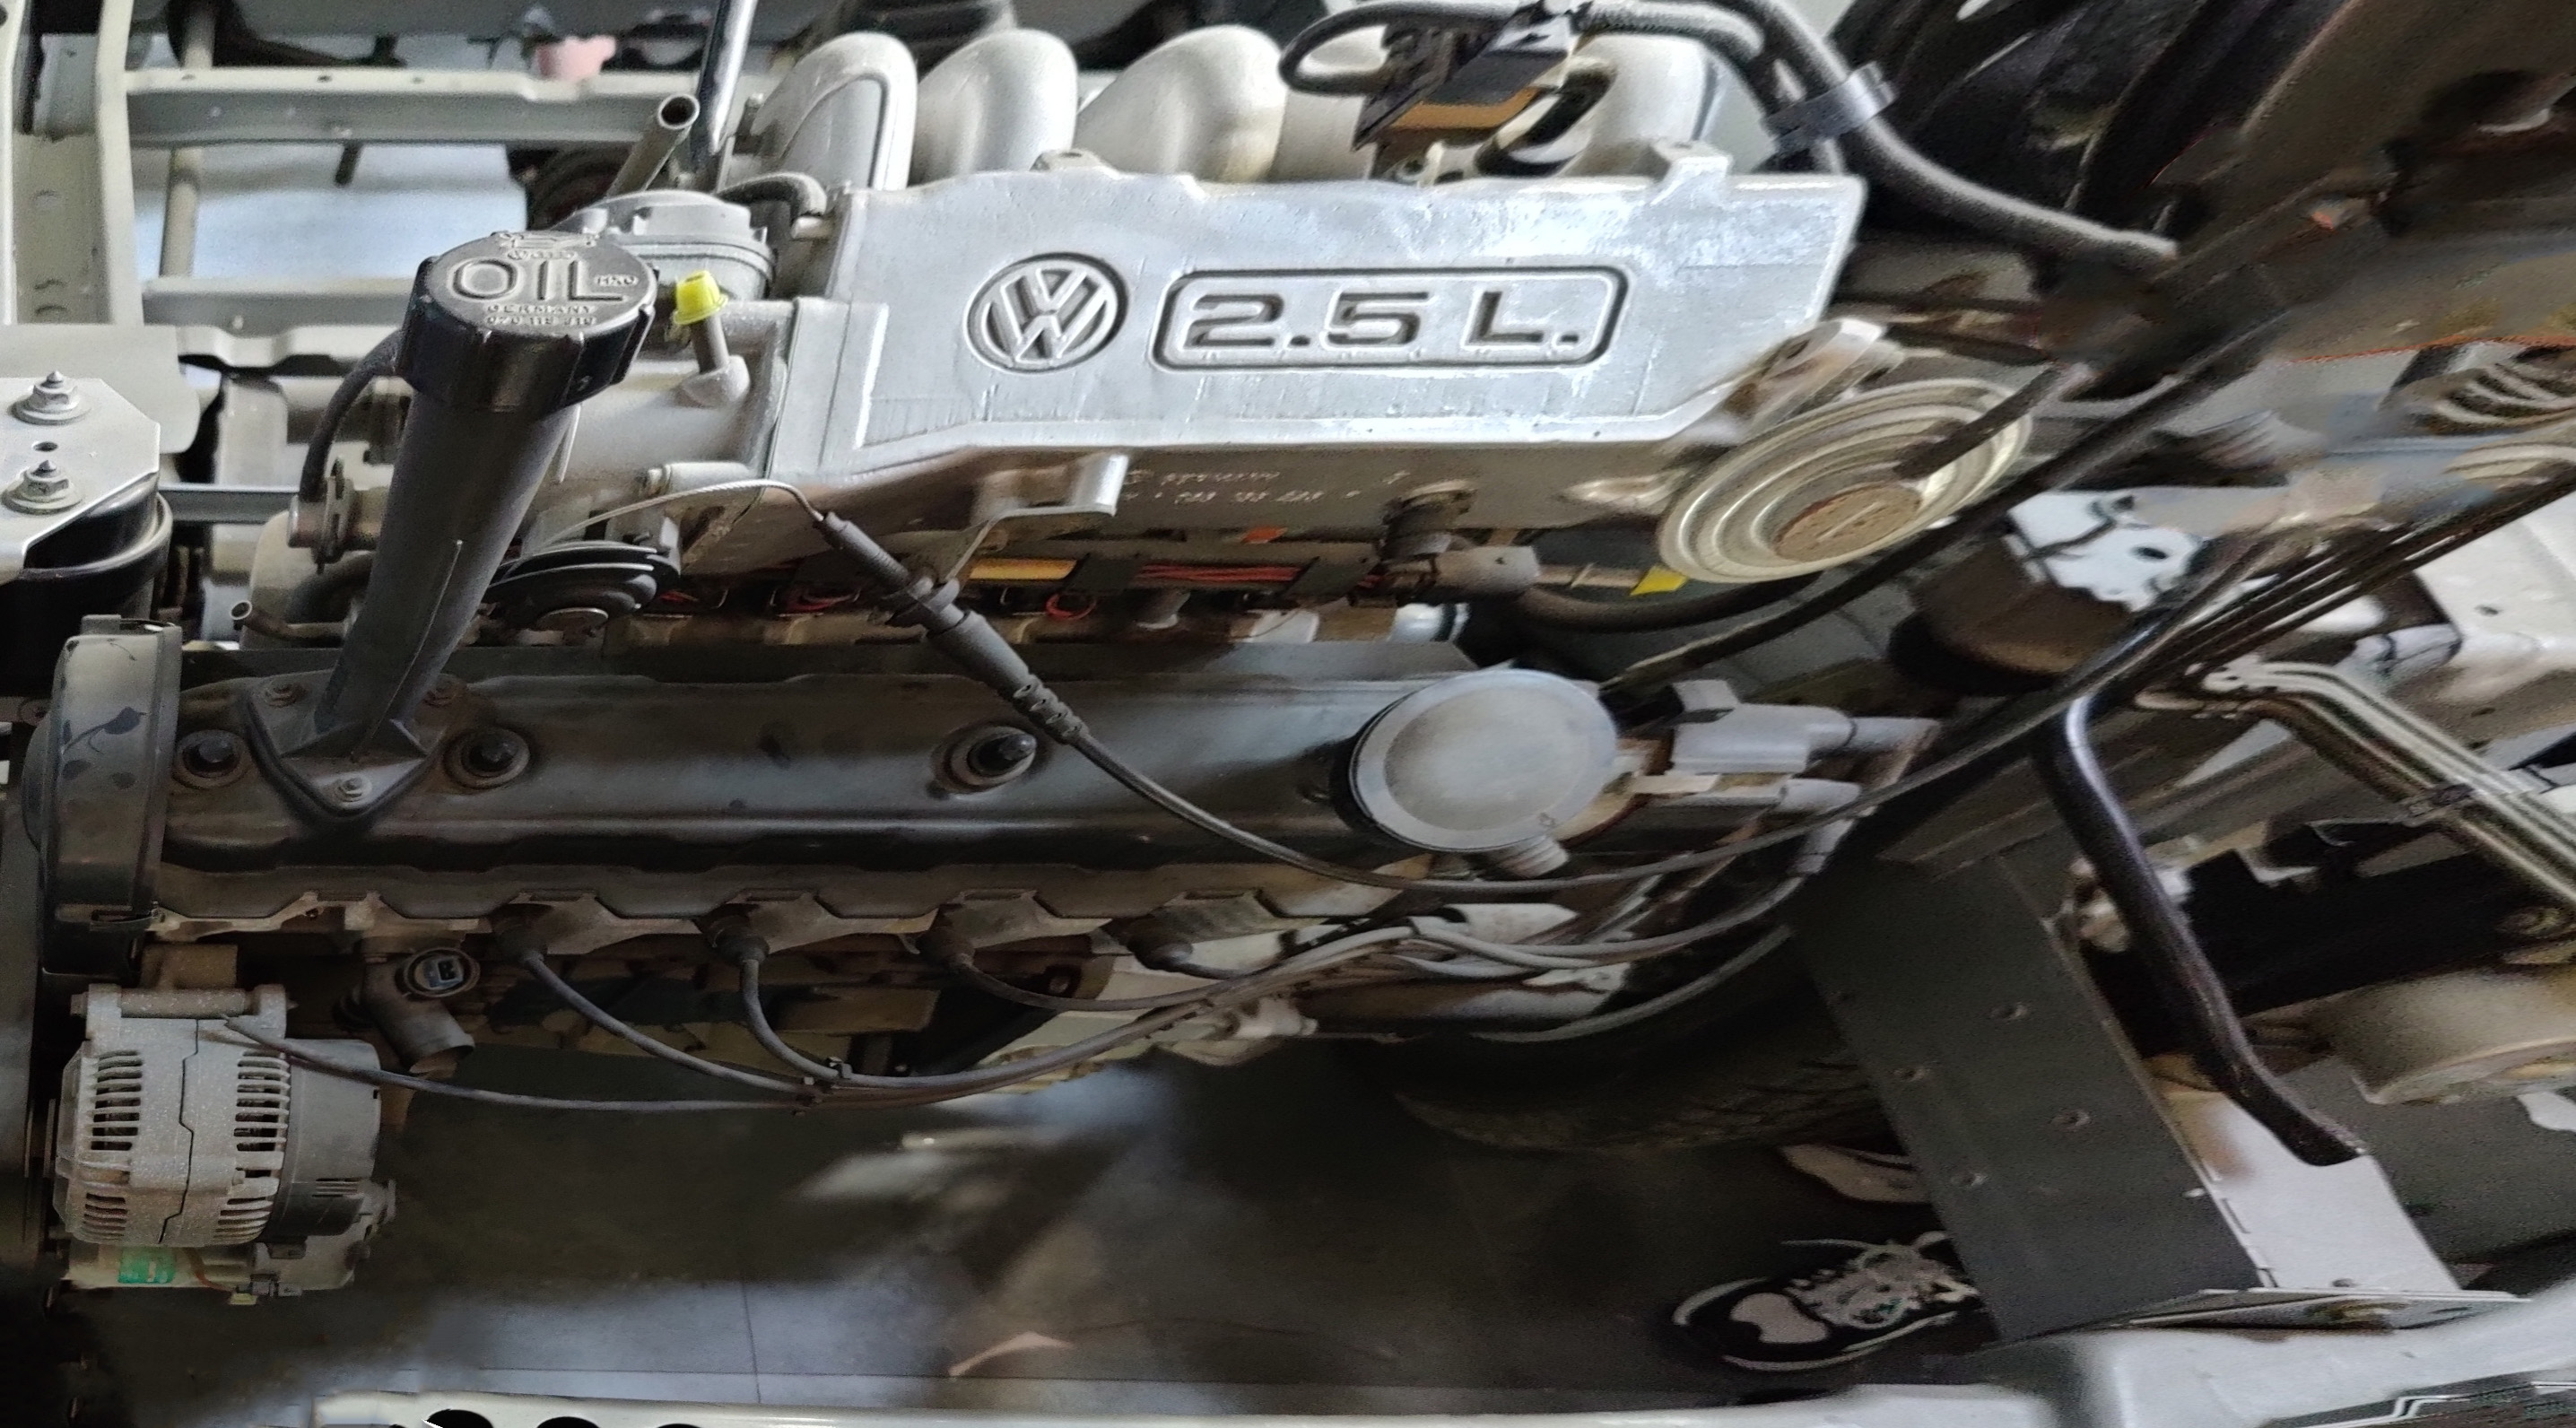
\includegraphics[width=\textwidth]{engine compartment with floor}
		\caption{带底板的发动机舱}
		\label{engine compartment with floor}
	\end{minipage}
\end{figure}

车身是一件精致的艺术品,以其优雅的雕塑形体、装饰件和内部覆饰以及悦目的色彩使人获得美感享受,反映时代的风貌、民族的传统和独特的企业形象。每辆车前后都有车标,但很多时候我们看清车标前就已能知道车辆的品牌。宝马的前脸、普桑的尾灯、法拉利的赛车红、劳斯莱斯的欢庆女神,凡此种种都已成为一款车家族性的标志。

现在乘用车常用承载式车身,车身还得承担起车架的功能,包括支撑连接汽车的各零部件、并承受来自车内外的各种载荷。车身既要承力,又要尽可能地轻量化,对现代的车身设计提出了更高要求。

% \subsection{请简述自动变速箱的换挡离合器和换挡制动器的主要组成部分及其工作原理。}
% \subsection{请简述增压发动机进气系统的主要组成部分及其功能。}
\newpage

\section{变速箱部分}
\subsection{手动变速器一般有哪些档位? 试述各档的动力传递路线。}

\label{subsection:2.1}

手动变速器一般为普通齿轮式变速器,也称轴线固定式变速器,它按照变速器传动齿轮轴的数目,可分为两轴式变速器和三轴式变速器(也称中间轴式变速器)。目前,轿车和轻、中型货车变速器通常有\numrange[range-phrase = $\,\sim\,$]{3}{5}个前进挡和一个倒挡,重型货车用组合式变速器中会有更多的挡位。三轴式变速器有真正的直接挡,部分变速器还设传动比小于1的超速挡,供良好路面行驶用。一般我们说的变速器挡位数,都指的是前进挡位数。

\cref{two-shaft manual transmission}为一用于纵置发动机的两轴式变速器(注意到图上注为2/3挡同步器的实为3/4挡同步器),和我们在拆装实践中用的那一型结构十分相似,动力传动路线也已在图中标出。对于该变速器:\\
1挡的动力传递路线为:输入轴(包括其上的1挡齿轮)$\rightarrow$输出轴1挡齿轮$\rightarrow$接合齿圈$\rightarrow$接合套$\rightarrow$花键毂$\rightarrow$输出轴;\\
2挡的动力传递路线为:输入轴(包括其上的2挡齿轮)$\rightarrow$输出轴2挡齿轮$\rightarrow$接合齿圈$\rightarrow$接合套$\rightarrow$花键毂$\rightarrow$输出轴;\\
3挡的动力传递路线为:输入轴$\rightarrow$花键毂$\rightarrow$接合套$\rightarrow$接合齿圈$\rightarrow$输入轴3挡齿轮$\rightarrow$输出轴3挡齿轮$\rightarrow$输出轴;\\
4挡的动力传递路线为:输入轴$\rightarrow$花键毂$\rightarrow$接合套$\rightarrow$接合齿圈$\rightarrow$输入轴4挡齿轮$\rightarrow$输出轴4挡齿轮$\rightarrow$输出轴;\\
5挡的动力传递路线为:输入轴$\rightarrow$花键毂$\rightarrow$接合套$\rightarrow$接合齿圈$\rightarrow$输入轴5挡齿轮$\rightarrow$输出轴5挡齿轮$\rightarrow$输出轴;\\
倒挡的动力传递路线为:输入轴$\rightarrow$输入轴倒挡齿轮$\rightarrow$倒挡中间齿轮$\rightarrow$输出轴倒挡齿轮$\rightarrow$输出轴。

\begin{figure}[htbp]
	\centering
	\begin{minipage}[b]{\textwidth}
		\centering
		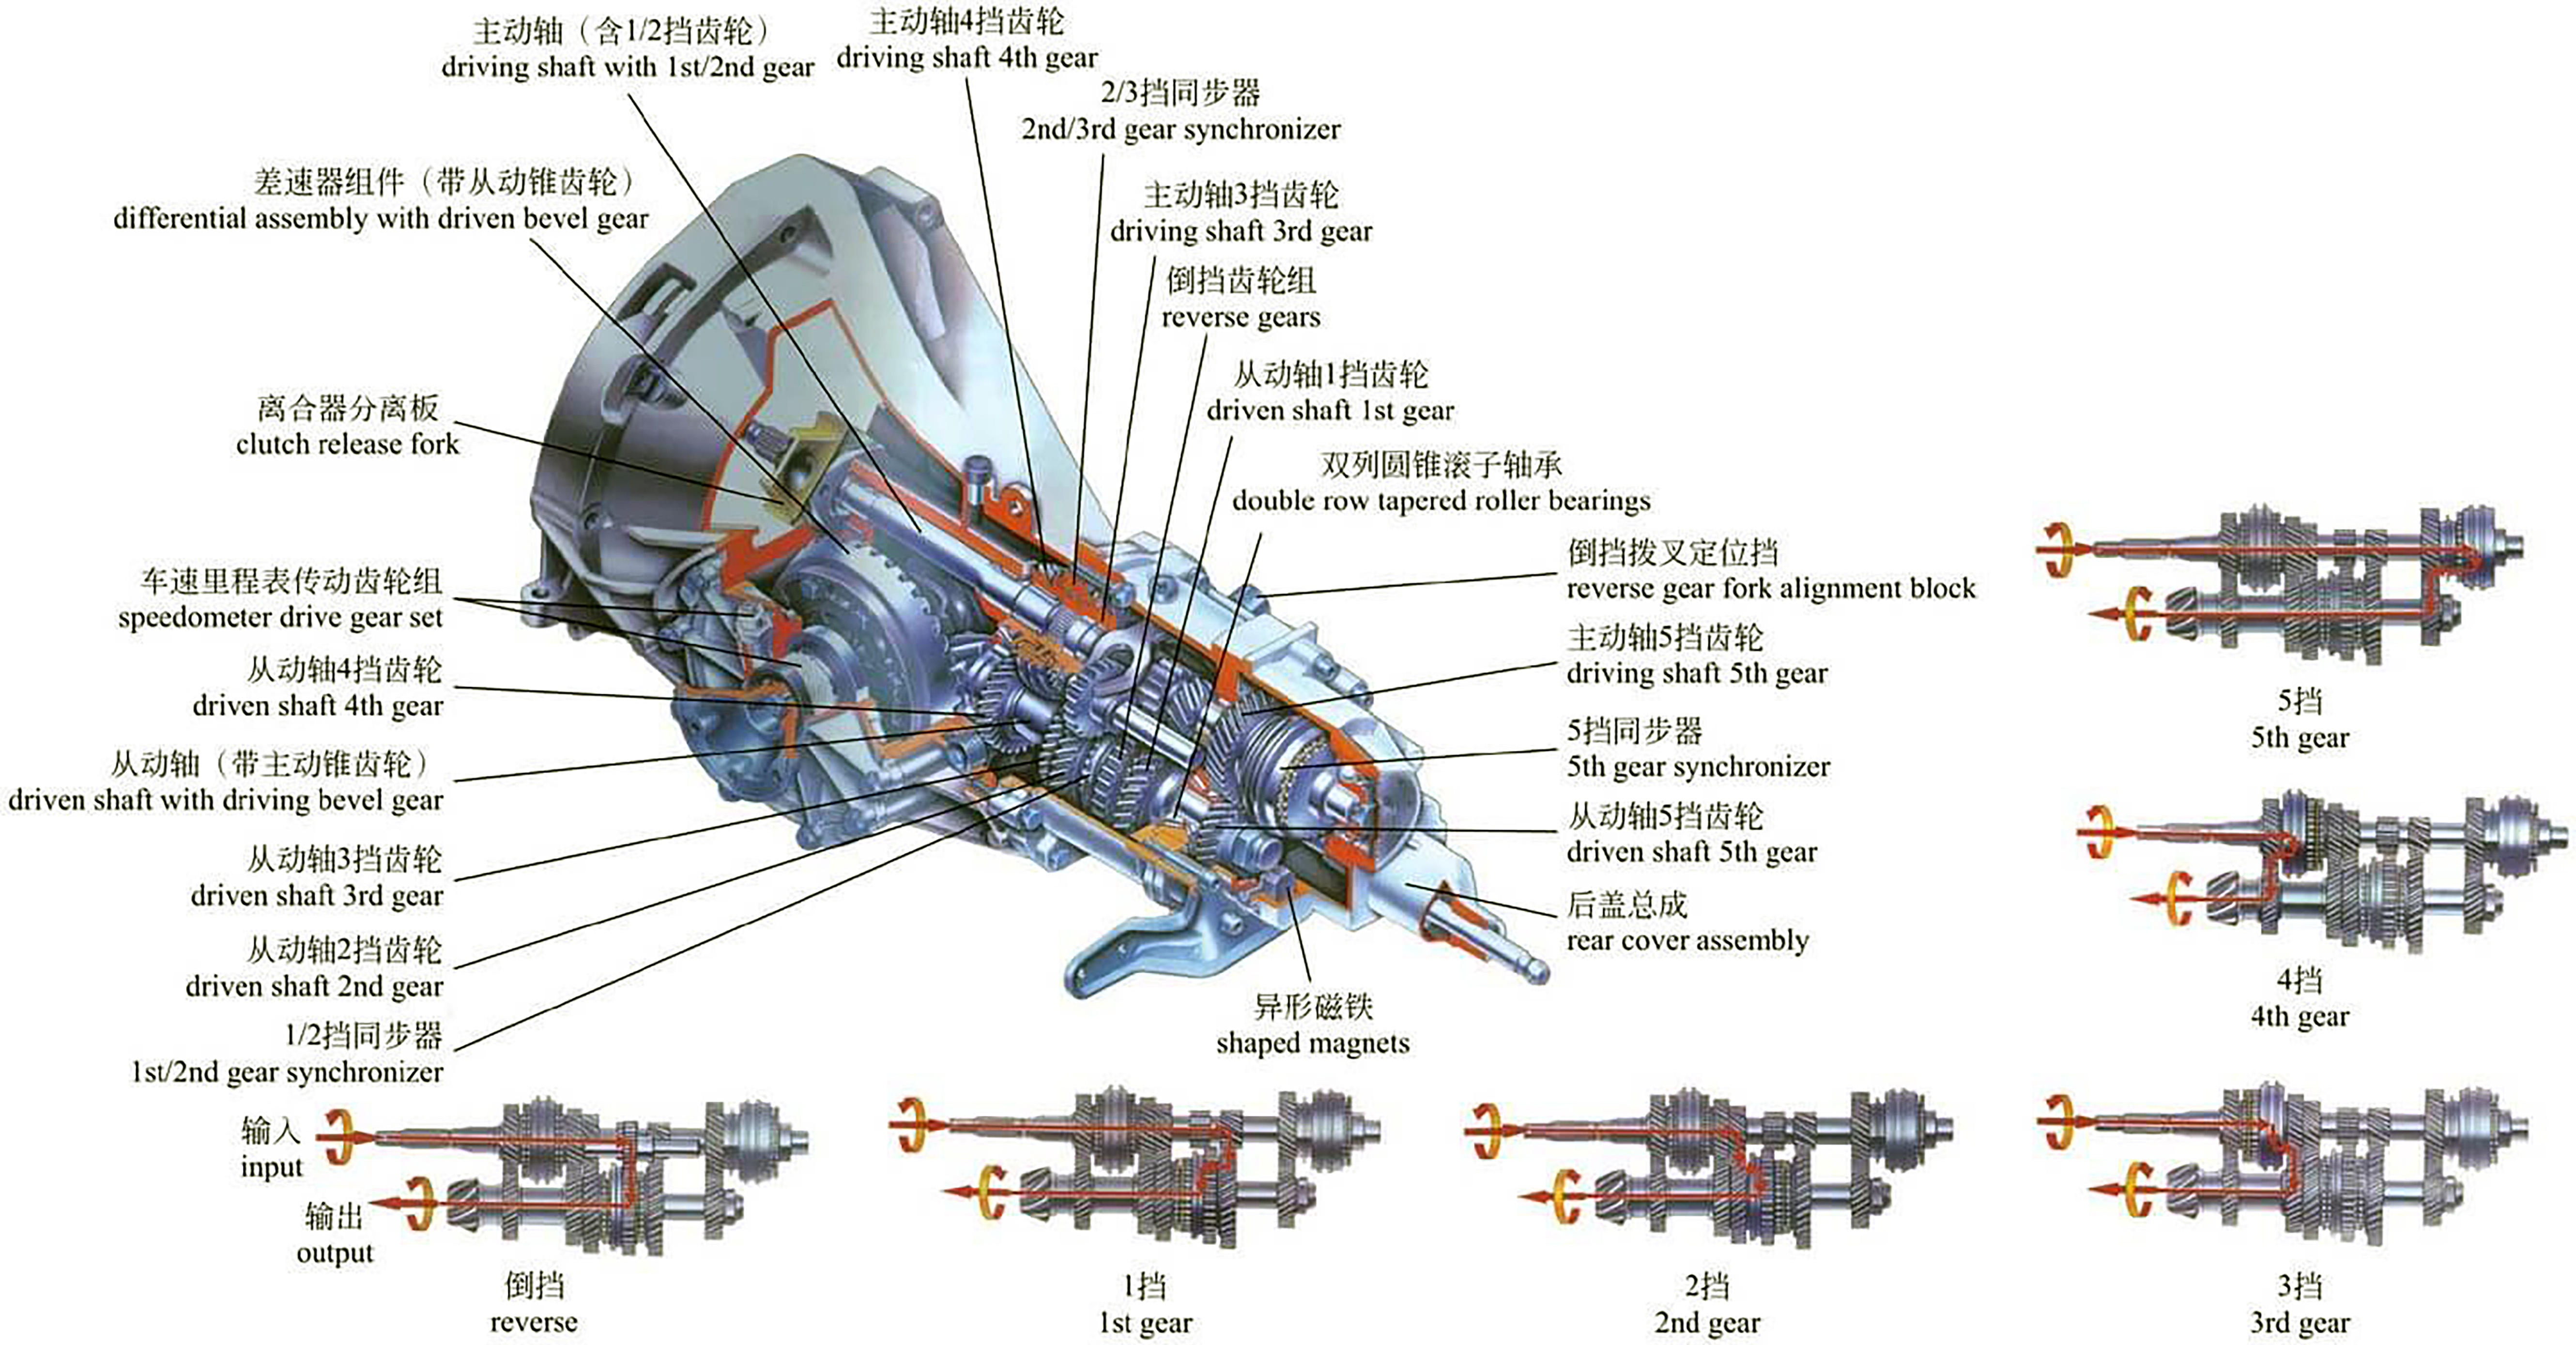
\includegraphics[width=\textwidth]{two-shaft manual transmission}
		\caption{两轴式5挡手动变速器}
		\label{two-shaft manual transmission}
	\end{minipage}
\end{figure}

\cref{three-shaft manual transmission}为课本上提到的一种三轴式变速器,它的特点是具有直接挡。在该变速器中,1、倒挡采用接合套换挡,其余各挡位采用同步器换挡,其中2挡使用锁销式同步器以承受更大载荷,\numrange[range-phrase = $\,\sim\,$]{3}{6}挡使用锁环式同步器。对该变速器:\\
1挡的动力传递路线为:第一轴$\rightarrow$第一轴常啮齿轮$\rightarrow$中间轴常啮齿轮$\rightarrow$中间轴$\rightarrow$中间轴1挡齿轮$\rightarrow$第二轴1挡齿轮$\rightarrow$接合齿圈$\rightarrow$接合套$\rightarrow$花键毂$\rightarrow$第二轴;\\
2挡的动力传递路线为:第一轴$\rightarrow$第一轴常啮齿轮$\rightarrow$中间轴常啮齿轮$\rightarrow$中间轴$\rightarrow$中间轴2挡齿轮$\rightarrow$第二轴2挡齿轮$\rightarrow$接合齿圈$\rightarrow$接合套$\rightarrow$花键毂$\rightarrow$第二轴;\\
3挡的动力传递路线为:第一轴$\rightarrow$第一轴常啮齿轮$\rightarrow$中间轴常啮齿轮$\rightarrow$中间轴$\rightarrow$中间轴3挡齿轮$\rightarrow$第二轴3挡齿轮$\rightarrow$接合齿圈$\rightarrow$接合套$\rightarrow$花键毂$\rightarrow$第二轴;\\
4挡的动力传递路线为:第一轴$\rightarrow$第一轴常啮齿轮$\rightarrow$中间轴常啮齿轮$\rightarrow$中间轴$\rightarrow$中间轴4挡齿轮$\rightarrow$第二轴4挡齿轮$\rightarrow$接合齿圈$\rightarrow$接合套$\rightarrow$花键毂$\rightarrow$第二轴;\\
5挡的动力传递路线为:第一轴$\rightarrow$第一轴常啮齿轮$\rightarrow$中间轴常啮齿轮$\rightarrow$中间轴$\rightarrow$中间轴5挡齿轮$\rightarrow$第二轴5挡齿轮$\rightarrow$接合齿圈$\rightarrow$接合套$\rightarrow$花键毂$\rightarrow$第二轴;\\
6挡(直接挡)的动力传递路线为:第一轴$\rightarrow$第一轴常啮齿轮$\rightarrow$接合齿圈$\rightarrow$接合套$\rightarrow$花键毂$\rightarrow$第二轴;\\
倒挡的动力传递路线为:第一轴$\rightarrow$第一轴常啮齿轮$\rightarrow$中间轴常啮齿轮$\rightarrow$中间轴$\rightarrow$中间轴倒挡齿轮$\rightarrow$倒挡中间齿轮$\rightarrow$第二轴倒挡齿轮$\rightarrow$接合齿圈$\rightarrow$接合套$\rightarrow$花键毂$\rightarrow$第二轴。

\begin{figure}[htbp]
	\centering
	\begin{minipage}[b]{\textwidth}
		\centering
		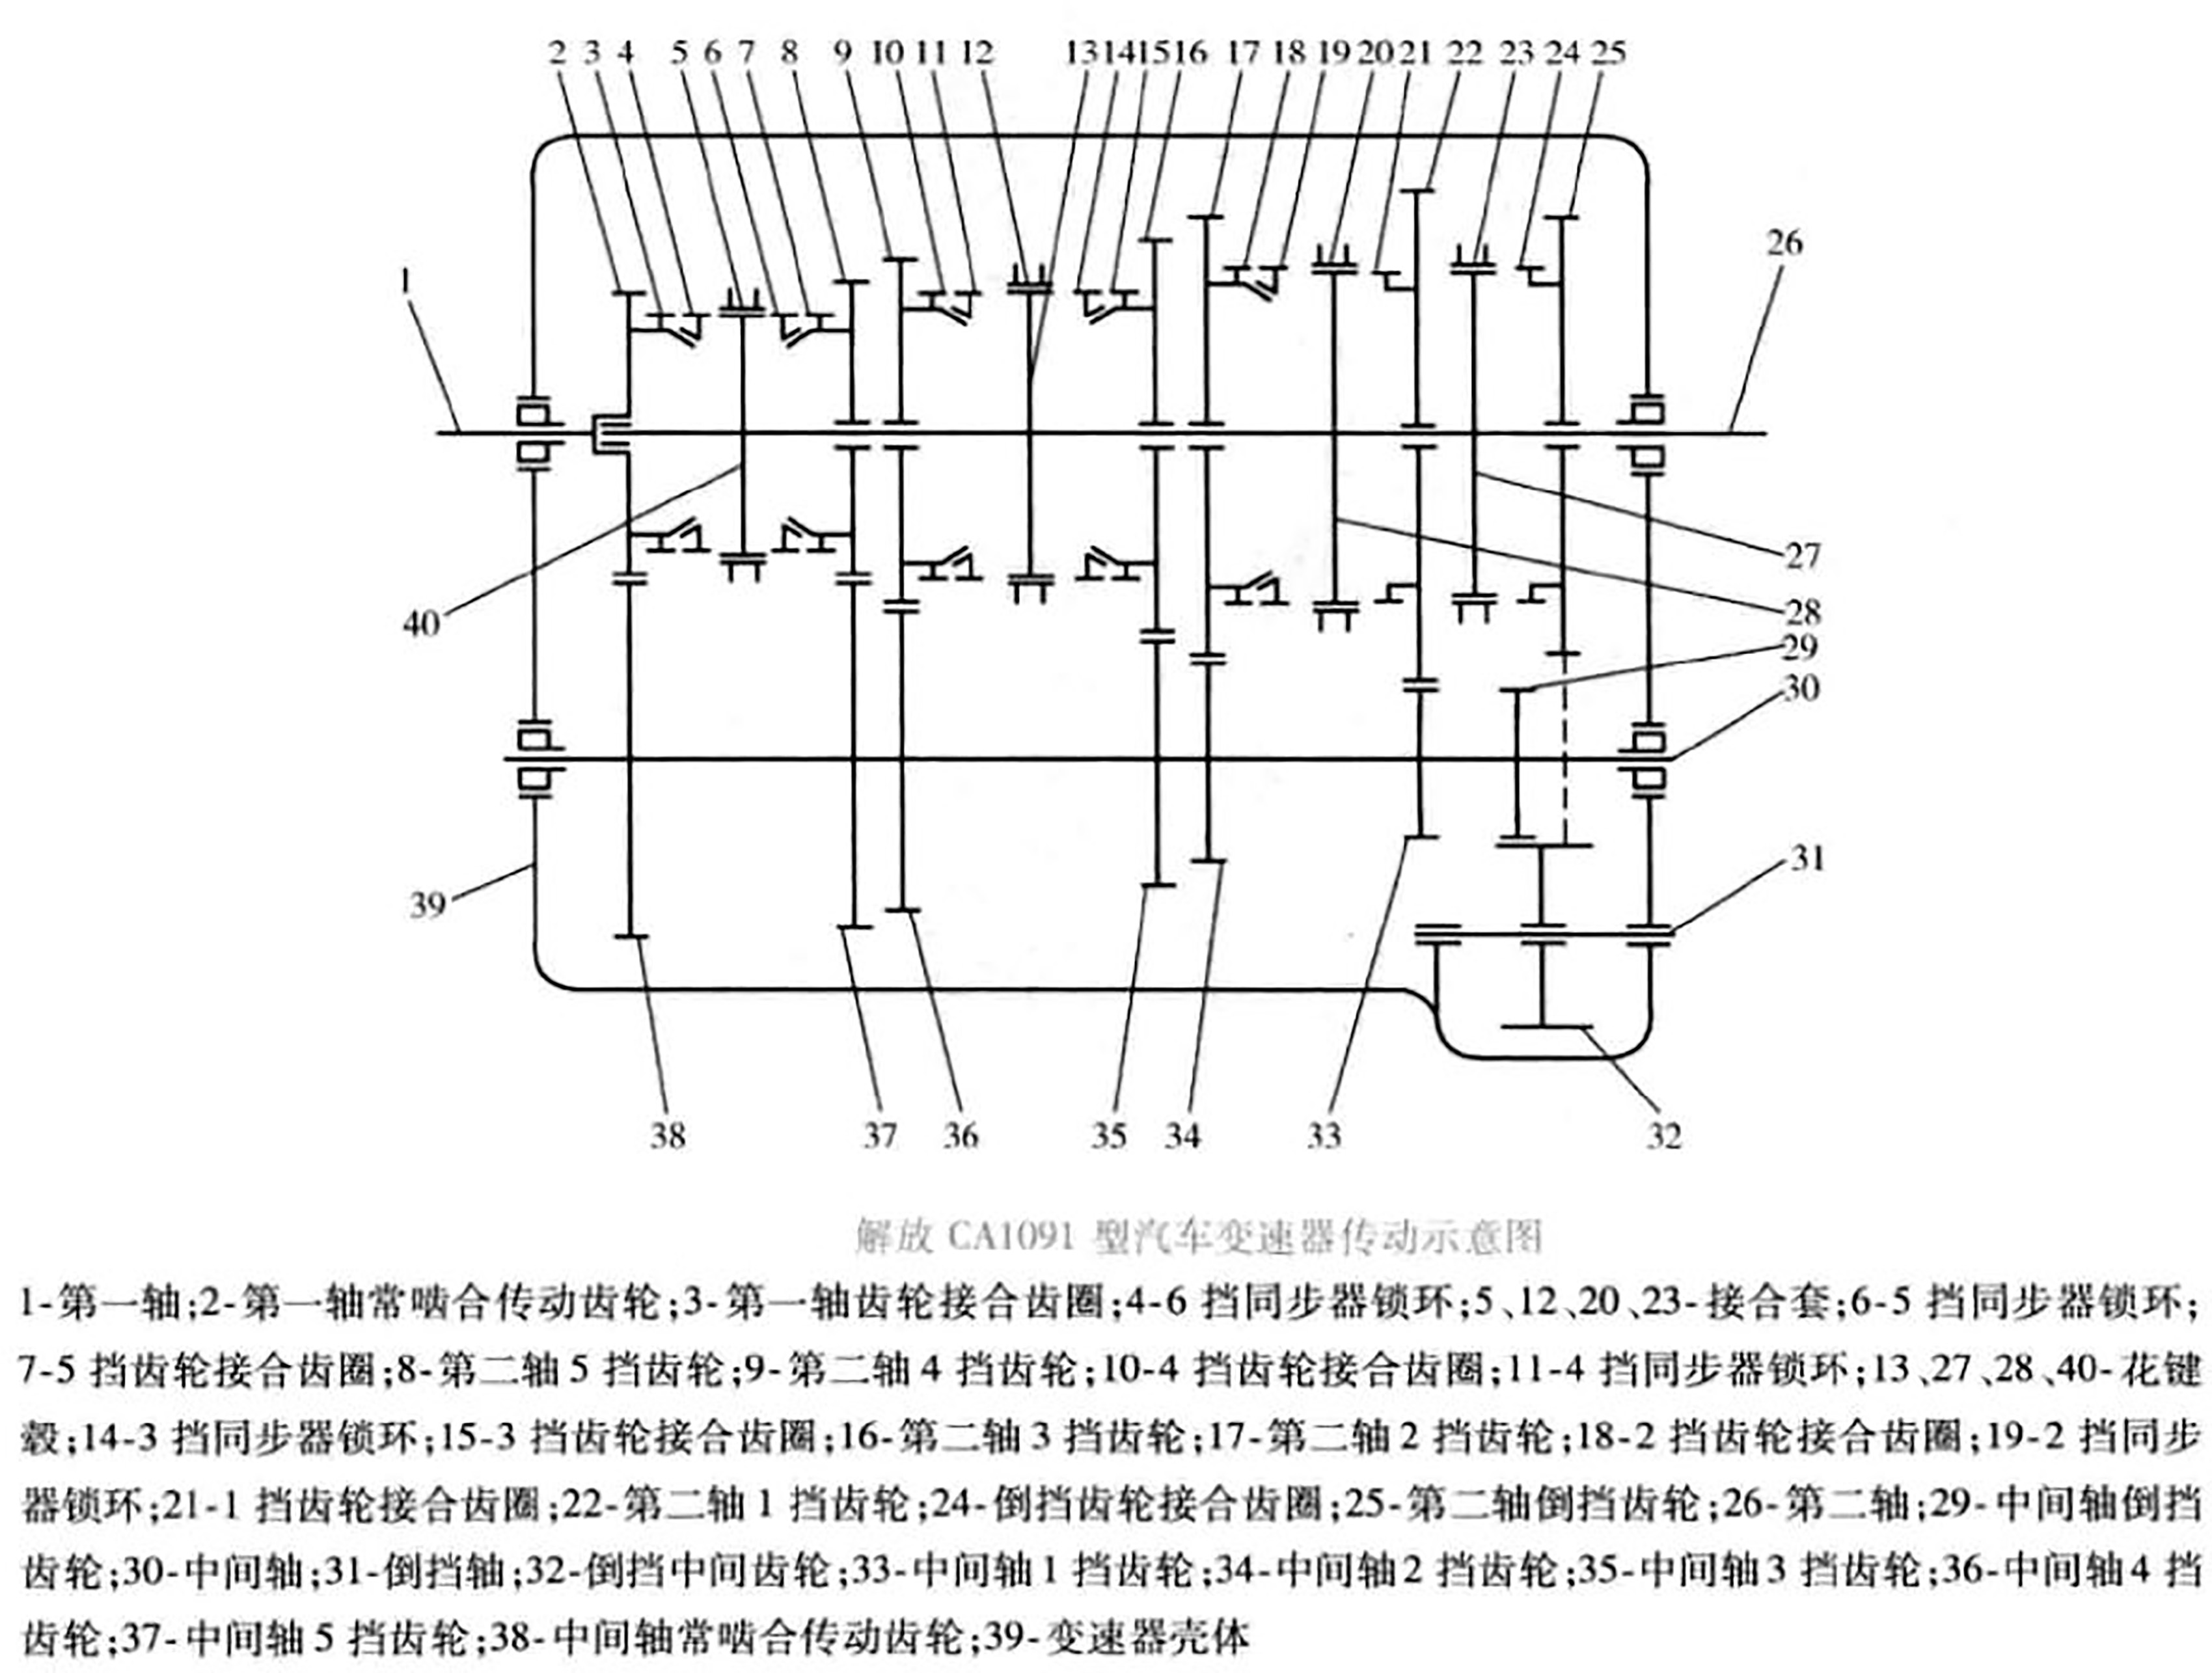
\includegraphics[width=\textwidth]{three-shaft manual transmission}
		\caption{三轴式6挡手动变速器}
		\label{three-shaft manual transmission}
	\end{minipage}
\end{figure}

\subsection{试述自锁与互锁装置的特点和作用。}

为保证变速器在任何情况下都能准确、安全、可靠地工作,其操纵机构必须设置安全装置,包括自锁、互锁和倒挡锁装置。对于六挡变速器,还应设置选挡锁装置。

自锁装置如\cref{self-locking}所示,它的作用主要有三。一是保证操纵变速杆推动拨叉前、后移动距离足够,使得滑动齿轮(或接合套)与相应的齿轮(或接合齿圈)在全齿宽上啮合,提高齿轮的寿命和承载力。二是保证在全齿宽啮合后汽车遇到较大颠簸或其它情况时,滑动齿轮(或接合套)不会自动产生轴向移动造成啮合长度的减小甚至是脱挡。三是为驾驶员提供良好的换挡手感,在钢球滑入凹槽后给驾驶员明显的反馈提示他换挡已到位。

自锁装置由自锁弹簧和自锁钢球组成,每根拨叉轴的表面有与钢球对应的凹槽(\cref{self-locking slots})。当任意一根拨叉轴连同拨叉一起轴向移动到空挡或某一工作挡位时,必有一个凹槽正对钢球,于是钢球被弹簧压嵌入该凹槽内,拨叉轴的轴向位置即被固定,从而拨叉连同滑动齿轮(或接合套)也被固定在空挡或一工作挡位上。当需要换挡时,驾驶员必须通过变速杆对拨叉和拨叉轴施加一定的轴力,这个力又在凹槽与拨叉轴接触的侧面上产生一克服弹簧弹力的纵向分力,将自锁钢球压回孔中,拨叉轴方可轴向移动。拨叉轴表面相邻自锁凹槽间的距离就等于使得在全齿宽上啮合或完全退出啮合所需的拨叉及拨叉轴的轴向移动距离。

注意到,该型变速器的1、2挡拨叉和3、4挡拨叉上均有三个自锁凹槽(\cref{self-locking slots}),中间的一个凹槽较浅,对应空挡,两边的凹槽较深,对应工作挡位。空挡的自锁凹槽较浅的原因可能是在空挡时与拨叉轴连接的滑动齿轮(或接合套)不参与动力传递,可能引起跳挡的干扰力小,且若某个拨叉轴已挂入工作挡位,其它拨叉轴的空挡位置即被互锁保证而无需过强的自锁。略感意外的是,5、倒挡拨叉轴上仅有两自锁凹槽,其中一个较浅,推测为空挡自锁,另一较深的应为5挡自锁。相信倒挡拨叉上有专供倒挡使用的自锁装置,不必在拨叉轴上实现倒挡自锁。

\begin{figure}[htbp]
	\centering
	\begin{minipage}[b]{0.6\textwidth}
		\centering
		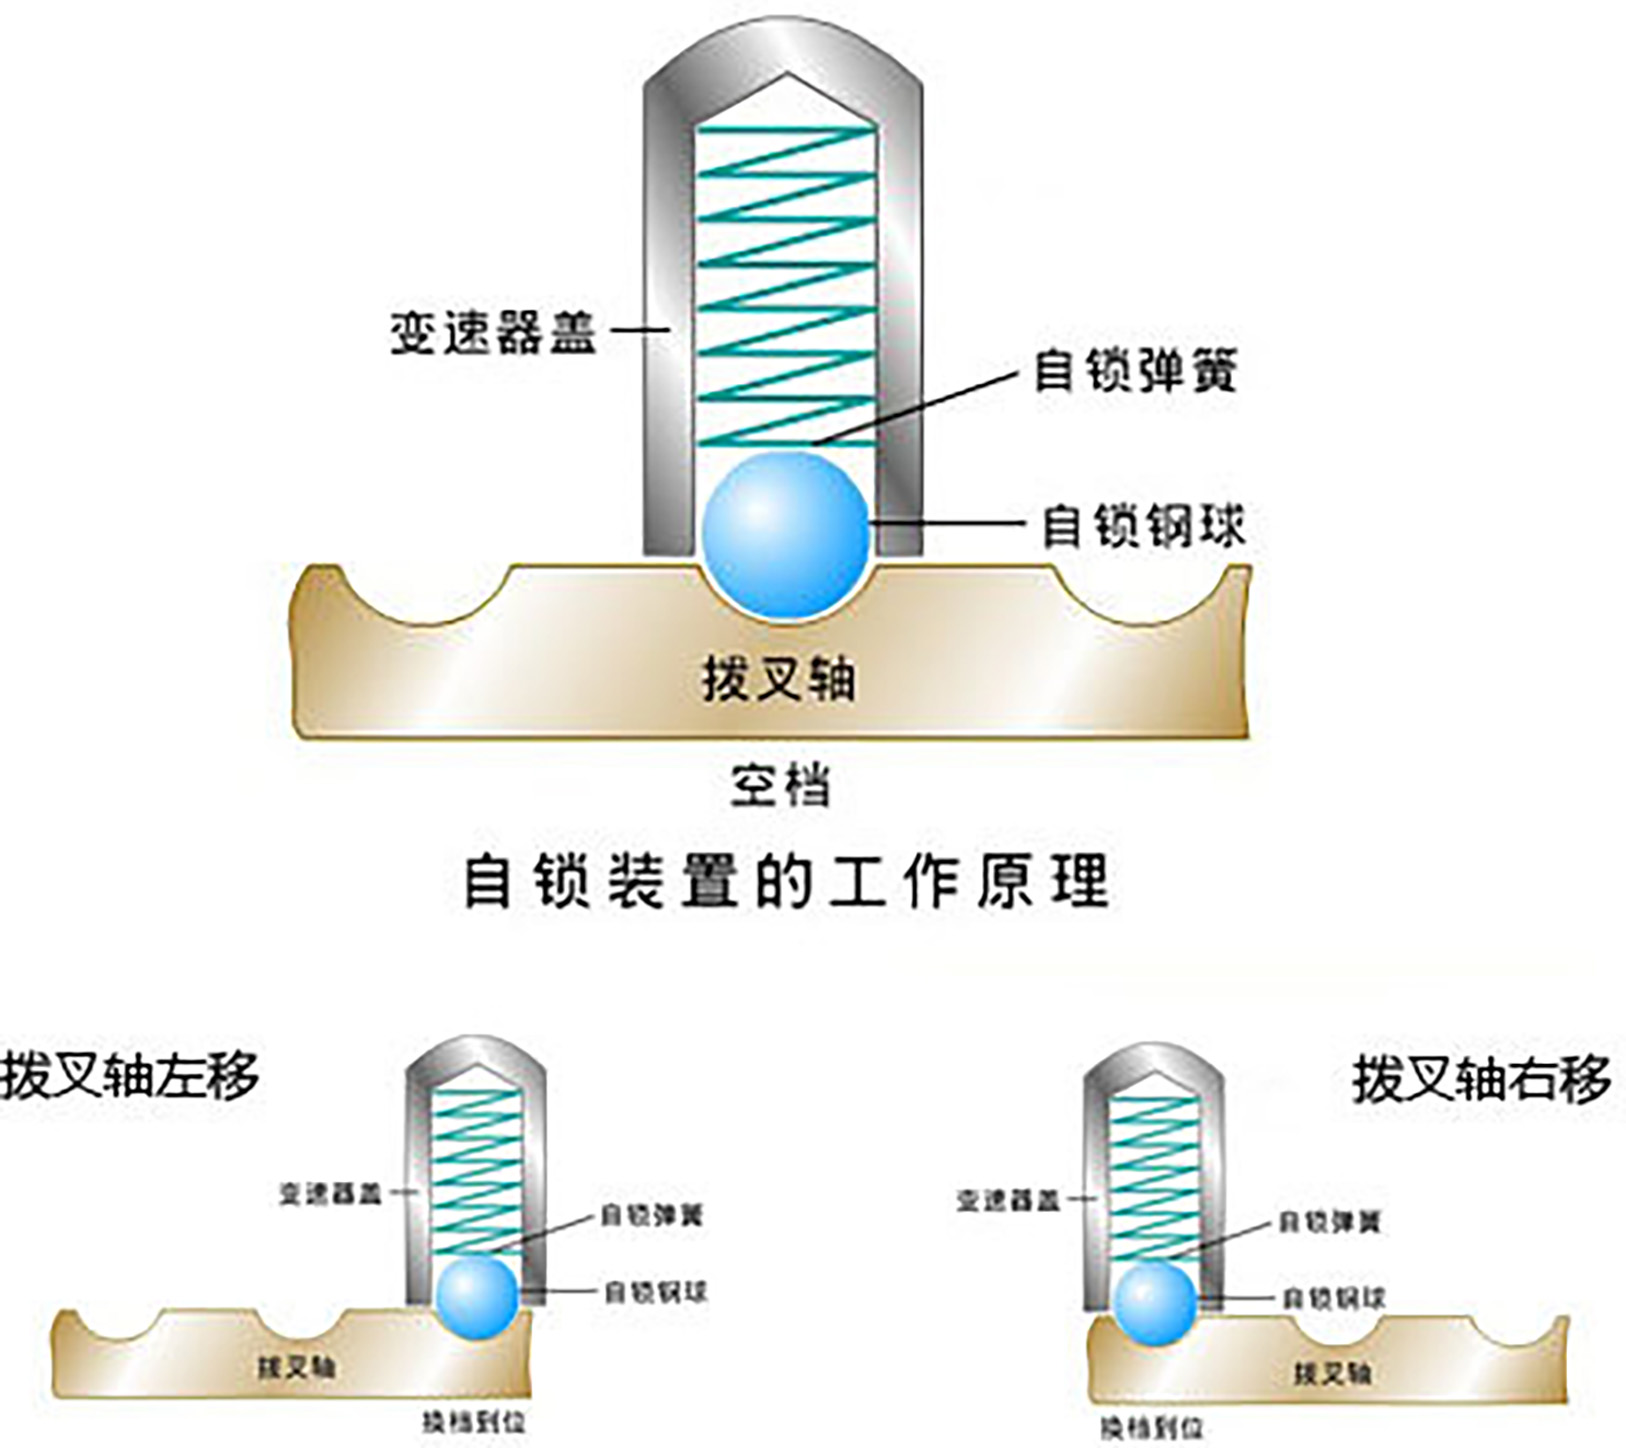
\includegraphics[width=\textwidth]{self-locking}
		\caption{自锁装置示意图}
		\label{self-locking}
	\end{minipage}
	\centering
	\begin{minipage}[b]{0.35\textwidth}
		\centering
		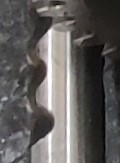
\includegraphics[width=\textwidth]{self-locking slots}
		\caption{自锁凹槽}
		\label{self-locking slots}
	\end{minipage}
	\begin{minipage}[b]{0.5\textwidth}
		\centering
		
\includegraphics[width=\textwidth]{self-locking slots 5R}
		\caption{5、倒挡拨叉轴上的自锁凹槽}
		\label{self-locking slots 5R}
	\end{minipage}
\end{figure}

互锁装置(\cref{interlocking})的作用就是防止变速器同时换入两个挡位。若变速杆能同时推动两个拨叉,则可同时换入两个挡位,但不同挡位的传动比不同,这样就会造成齿轮间的机械干涉,变速器被卡死,此时若传递的动力不消失,会使传动路线中最薄弱处被破坏,产生严重后果。

互锁装置由互锁钢球和互锁销组成,每根拨叉轴朝向互锁钢球的侧表面上均铣出一个深度相等的凹槽,任一拨叉轴处于空挡位置时其侧面凹槽都恰对准互锁钢球。两互锁钢球直径之和等于相邻两轴表面间距离加一凹槽深度。中间拨叉轴上两互锁凹槽间有一孔将二者连同,孔中置有互锁销,销的长度等于拨叉轴的直径减去一凹槽深。当变速器处于空挡时,互锁凹槽、互锁钢球和互锁销都在同一直线上。当移动中间那根拨叉轴时,轴两侧的内互锁钢球被从凹槽中挤出,推动外互锁钢球分别嵌入外侧两根拨叉轴侧面的互锁凹槽中,将两轴锁止在空挡位置。如此时欲像\cref{interlocking}中右侧子图所示那样移动1、2挡拨叉轴,则须先将中间的3、4挡拨叉轴退回空挡位置,再移动1、2挡拨叉轴,互锁钢球便被从1、2挡拨叉轴上的互锁凹槽挤出,推动互锁销和其它互锁钢球将剩余两拨叉轴锁止于空挡。\cref{interlocking}中推动倒挡拨叉轴的过程也类似。可见,互锁装置结构的设计使得驾驶员用变速杆推动某一拨叉轴时能自动锁止其它所有拨叉轴。

在我们的拆装实践中,事实上互锁销和互锁钢球都已被提前取出,我们只能看到定位互锁钢球的凹槽和通互锁销的小孔。减速器中互锁装置和自锁装置做在一起,都位于拨叉轴的安装孔上。自锁弹簧和自锁钢球组成一部件,拨叉轴被取出后仍能保持在变速器盖中而不脱出;但互锁销和互锁钢球都是分立零件,体积很小,且依赖拨叉轴固定,在拆卸中易被遗失。在自锁和互锁都存在的情况下,拨叉轴当然还是可以安装的,但须保证装入最后一根拨叉轴时,另两轴都位于空挡位置,否则会发生干涉。

\begin{figure}[htbp]
	\centering
	\begin{minipage}[b]{0.65\textwidth}
		\centering
		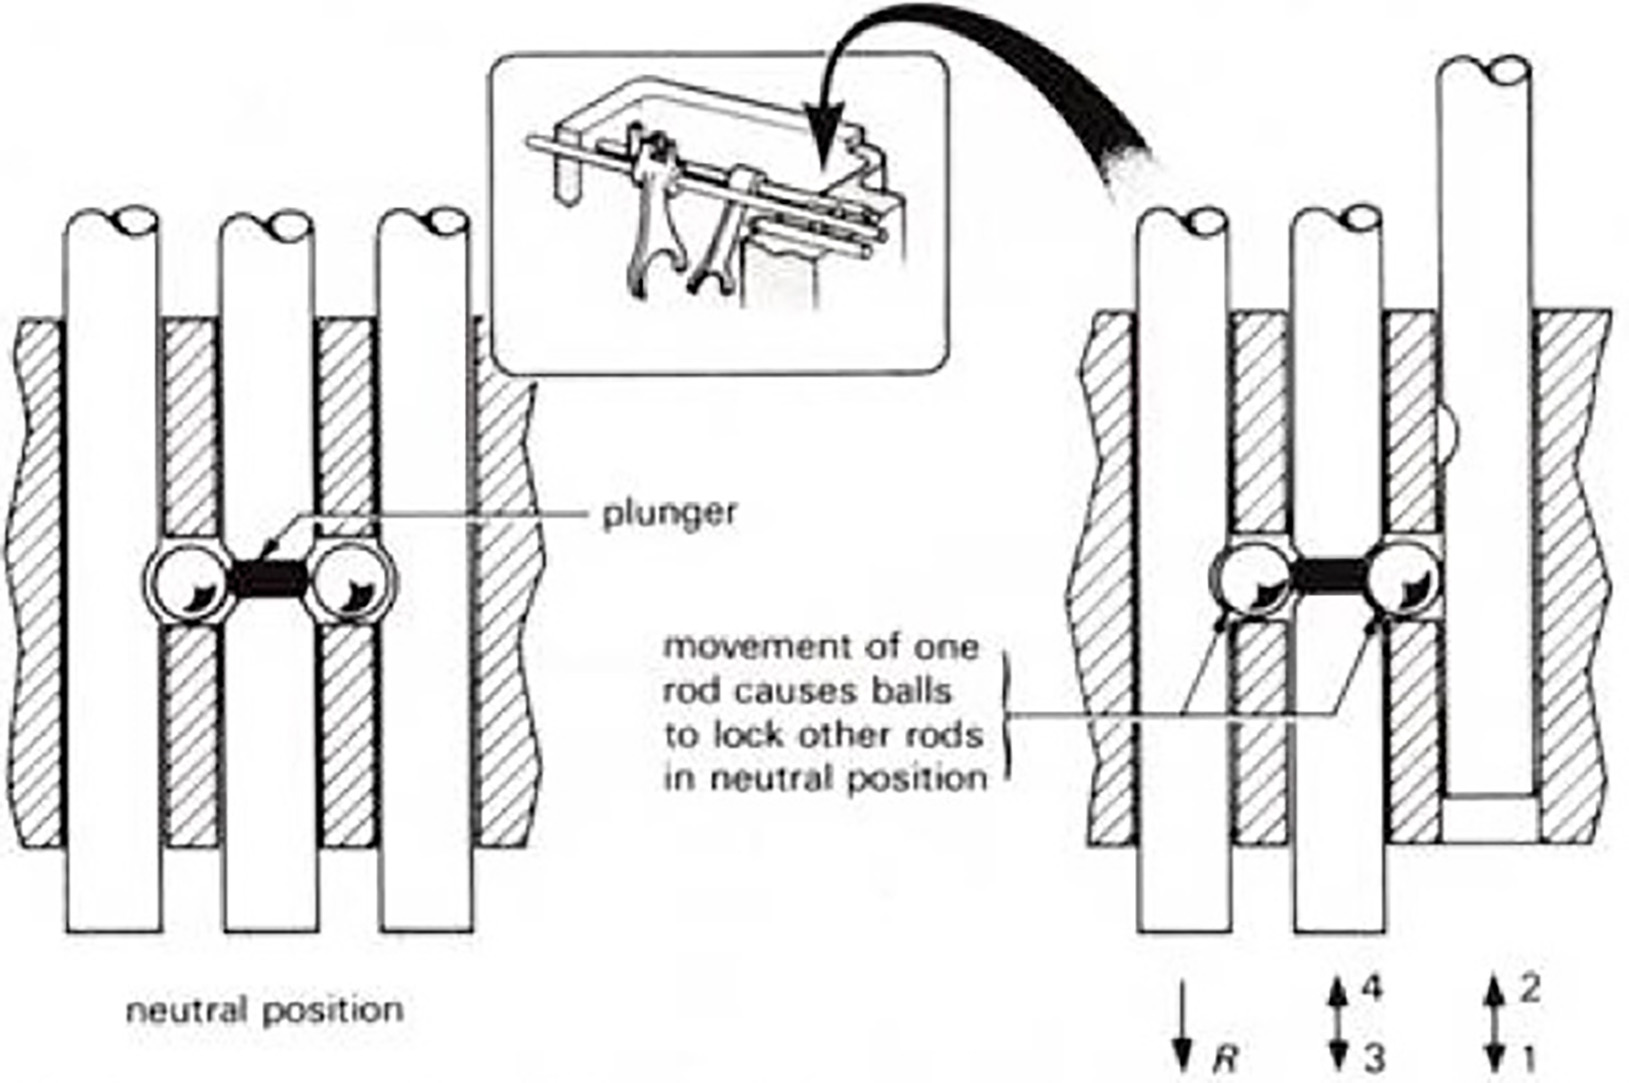
\includegraphics[width=\textwidth]{interlocking}
		\caption{互锁装置示意图}
		\label{interlocking}
	\end{minipage}
	\begin{minipage}[b]{0.3\textwidth}
		\centering
		\begin{minipage}[b]{0.8\textwidth}
			\centering
			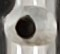
\includegraphics[width=\textwidth]{interlocking slot 34}
		\end{minipage}
		\begin{minipage}[b]{0.8\textwidth}
			\centering
			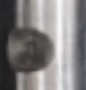
\includegraphics[width=\textwidth]{interlocking slot 5R}
		\end{minipage}
		\caption{互锁凹槽}
		\label{interlocking slots}
	\end{minipage}
\end{figure}

\subsection{试分析变速箱拆装过程的特点?}

在变速器的拆装过程中,最重要的就是记录下拆卸顺序,并在重新装配时严格按拆卸的倒序安装。

拆卸的顺序可根据各零件间相对位置关系确定。譬如说换挡轴是第一个被拆下的零件,但其上的拨杆会与5挡拨叉上的拨块干涉,需先将拨叉上的定位销取出以拆下拨叉,换挡轴在旋转一角度后便可从轴向抽出。变速器的输入轴(\cref{input shaft})和输出轴(\cref{output shaft})都是过盈装配在变速器壳体上的,拆卸时要借助压床将它们压出,压出时依次给输入、输出轴施加一小位移,并如此循环,直至两轴全被压出,注意避免让圆锥滚子轴承跳出。若一次只压一根轴,可能啮合的斜齿轮间会干涉造成齿轮损坏。输出轴被压出后,其上的1、2挡拨叉轴和拨叉才可被取下。输入轴上的3、4挡齿轮和相应的同步器由轴用挡圈轴向定位,其中固定输入轴4挡齿轮的卡簧上开有两孔,需将卡簧钳两尖头伸入孔中将卡簧撑开后提出,而固定花键毂的卡簧较厚,更好的方法是用专用的卡簧钳摩擦力较大的成平面的两侧面撑开卡簧缺口后取出。卡簧的拆装较为困难,且如果盲目撬开会造成卡簧变形,无法再装上。变速器上用到的三个定位销(\cref{location pins})为弹性圆柱销,中空且母线方向上有一贯穿的缺口。将销钉敲下时,应用磨钝尖端的螺钉抵住销钉边缘,并用锤子敲击螺钉头部。若直接让螺钉深伸入定位销中部的孔用力,可能会撑大定位销,使之难以被取出。

重新装配变速器的过程事实上较拆卸有更多需要注意的点,因为拆卸顺序错误无非是有零件无法拆下,但装配错误可能要到后面试图装其它零件时才能发现,所幸我组没有遇到此类情况。该型变速器上所用同步器的滑块靠两侧的两钢丝弹簧固定,钢丝弹簧开口的一端有一倒钩,另一端是平的。装配同步器时,先将滑块放入花键毂的凹槽中,套上接合套将滑块基本限位住后才能安装钢丝弹簧。安装钢丝弹簧时,要首先让其有钩子的一端钩住滑块背面的凹槽,然后将其余部分压入,这使得钢丝弹簧不会在同步器中周向转动,也不会从轴向脱出。注意到钢丝弹簧只有约3/4圆周长,故而在安装另一面的钢丝弹簧时注意将缺口错开,以免滑块受力不均。我们主要探究的是3、4挡同步器,这个同步器虽向两侧均能工作,分别控制3、4挡,但仔细观察会发现其花键毂的外花键是断开的,外花键两侧不等长,且花键毂的两侧毂与外花键端部的距离不等,总之花键毂并非左右对称。这种设计可能的原因是两挡受力不同,也带来了安装方向的问题。若将同步器翻转过来安装,花键毂能被装上,因为用于定位花键毂的毂翻转后长度不变,但花键毂上外花键端部的位置变了,这就会使得4挡齿轮装不上,又得把同步器整体拆下重装。所以拆卸时就应记下该同步器的方向以便后面的安装。装回输入、输出轴时,自然要和拆下时一样先把两轴摆到齿轮能啮合的位置,且输出轴要带着1、2挡拨叉轴和拨叉一道装回。然而,装回输入、输出轴时压床已不可用,因为轴伸出箱体的长度超出了压床的工作范围。我们采用的办法是将轴的一端顶在台虎钳上,另一侧用套筒顶在放入轴安装孔的轴承上,敲击套筒即可借助相对运动把输入、输出轴安装到位。倒挡轴和倒挡中间齿轮拆下时较易,仅需将倒挡轴敲出,但装入时要确定倒挡齿轮的方向,且因此时输入、输出轴已装上,倒挡齿轮放倒后才能装入,需用螺丝刀将齿轮重新挑到直立位后再装入倒挡轴。由于倒挡轴上带有定位销,装入时销钉要对准壳体上的开槽,且要从倒挡齿轮的另一侧装入,避免定位销和倒挡齿轮干涉。变速器中三个拨叉也都不是左右对称的,需按原方向安装,否则会和自锁干涉。我们的变速器中已拆掉了互锁,故两拨叉轴可同时挂入工作挡位,但为了最后变速杆安装方便和以后的拆卸,我们需将三轴均移至空挡位置。

\begin{figure}[htbp]
	\centering
	\begin{minipage}[b]{0.18\textwidth}
		\centering
		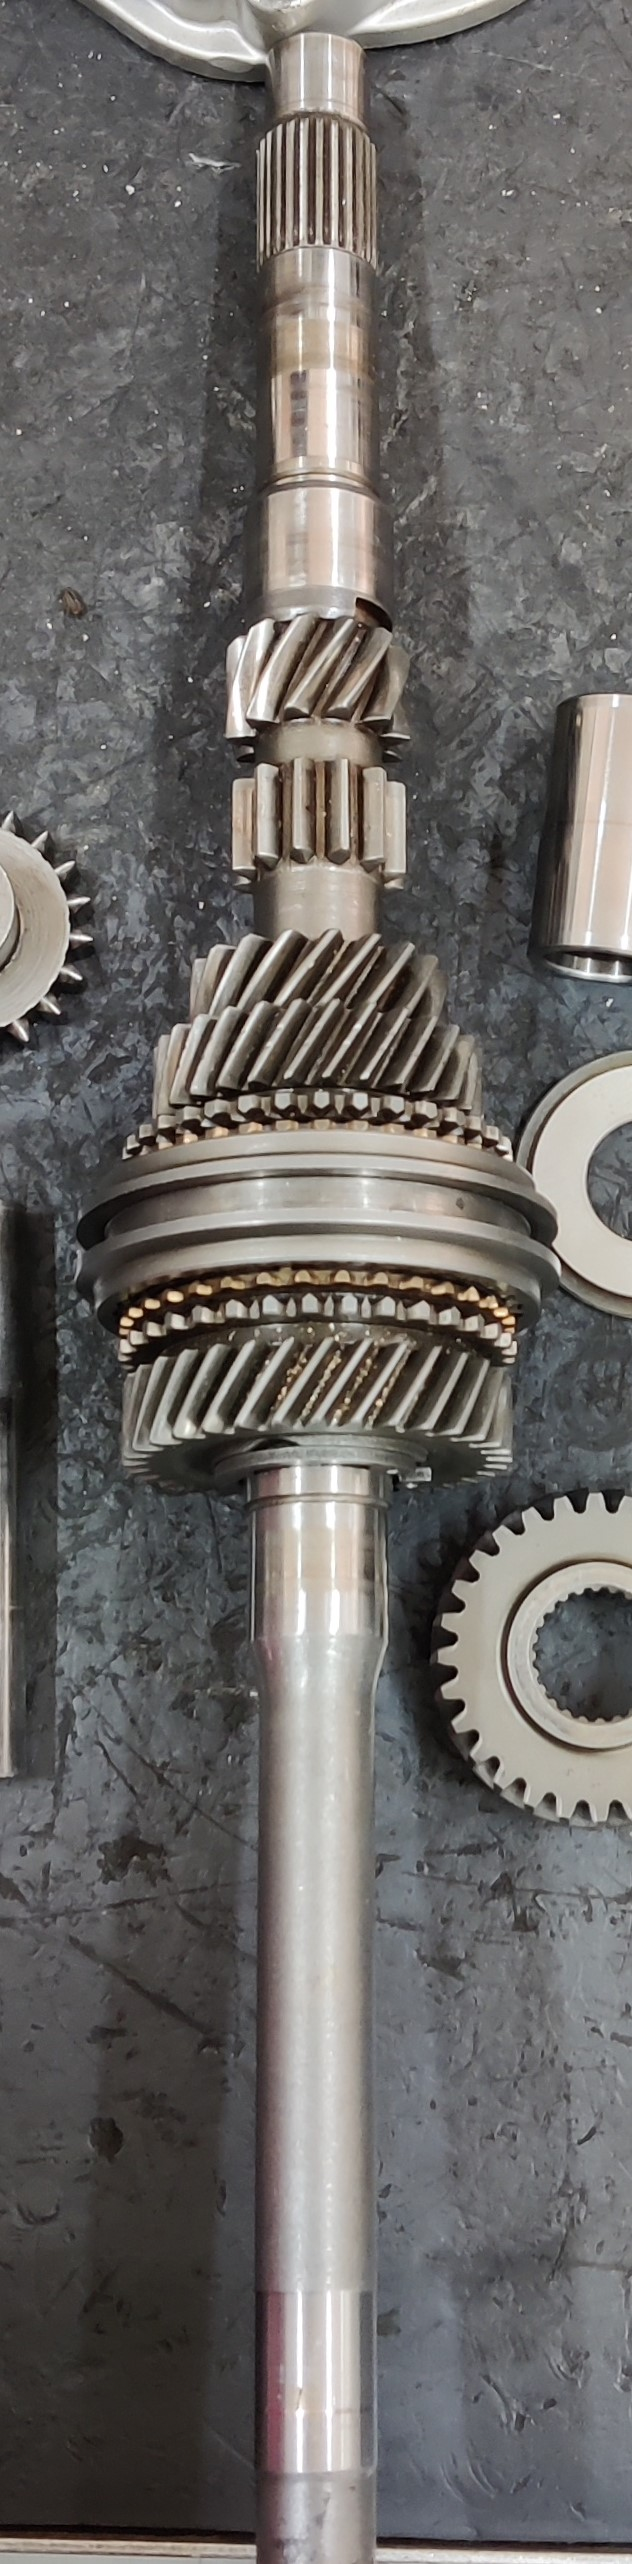
\includegraphics[width=\textwidth]{input shaft}
		\caption{输入轴}
		\label{input shaft}
	\end{minipage}
	\begin{minipage}[b]{0.31\textwidth}
		\centering
		\begin{minipage}[b]{\textwidth}
			\centering
			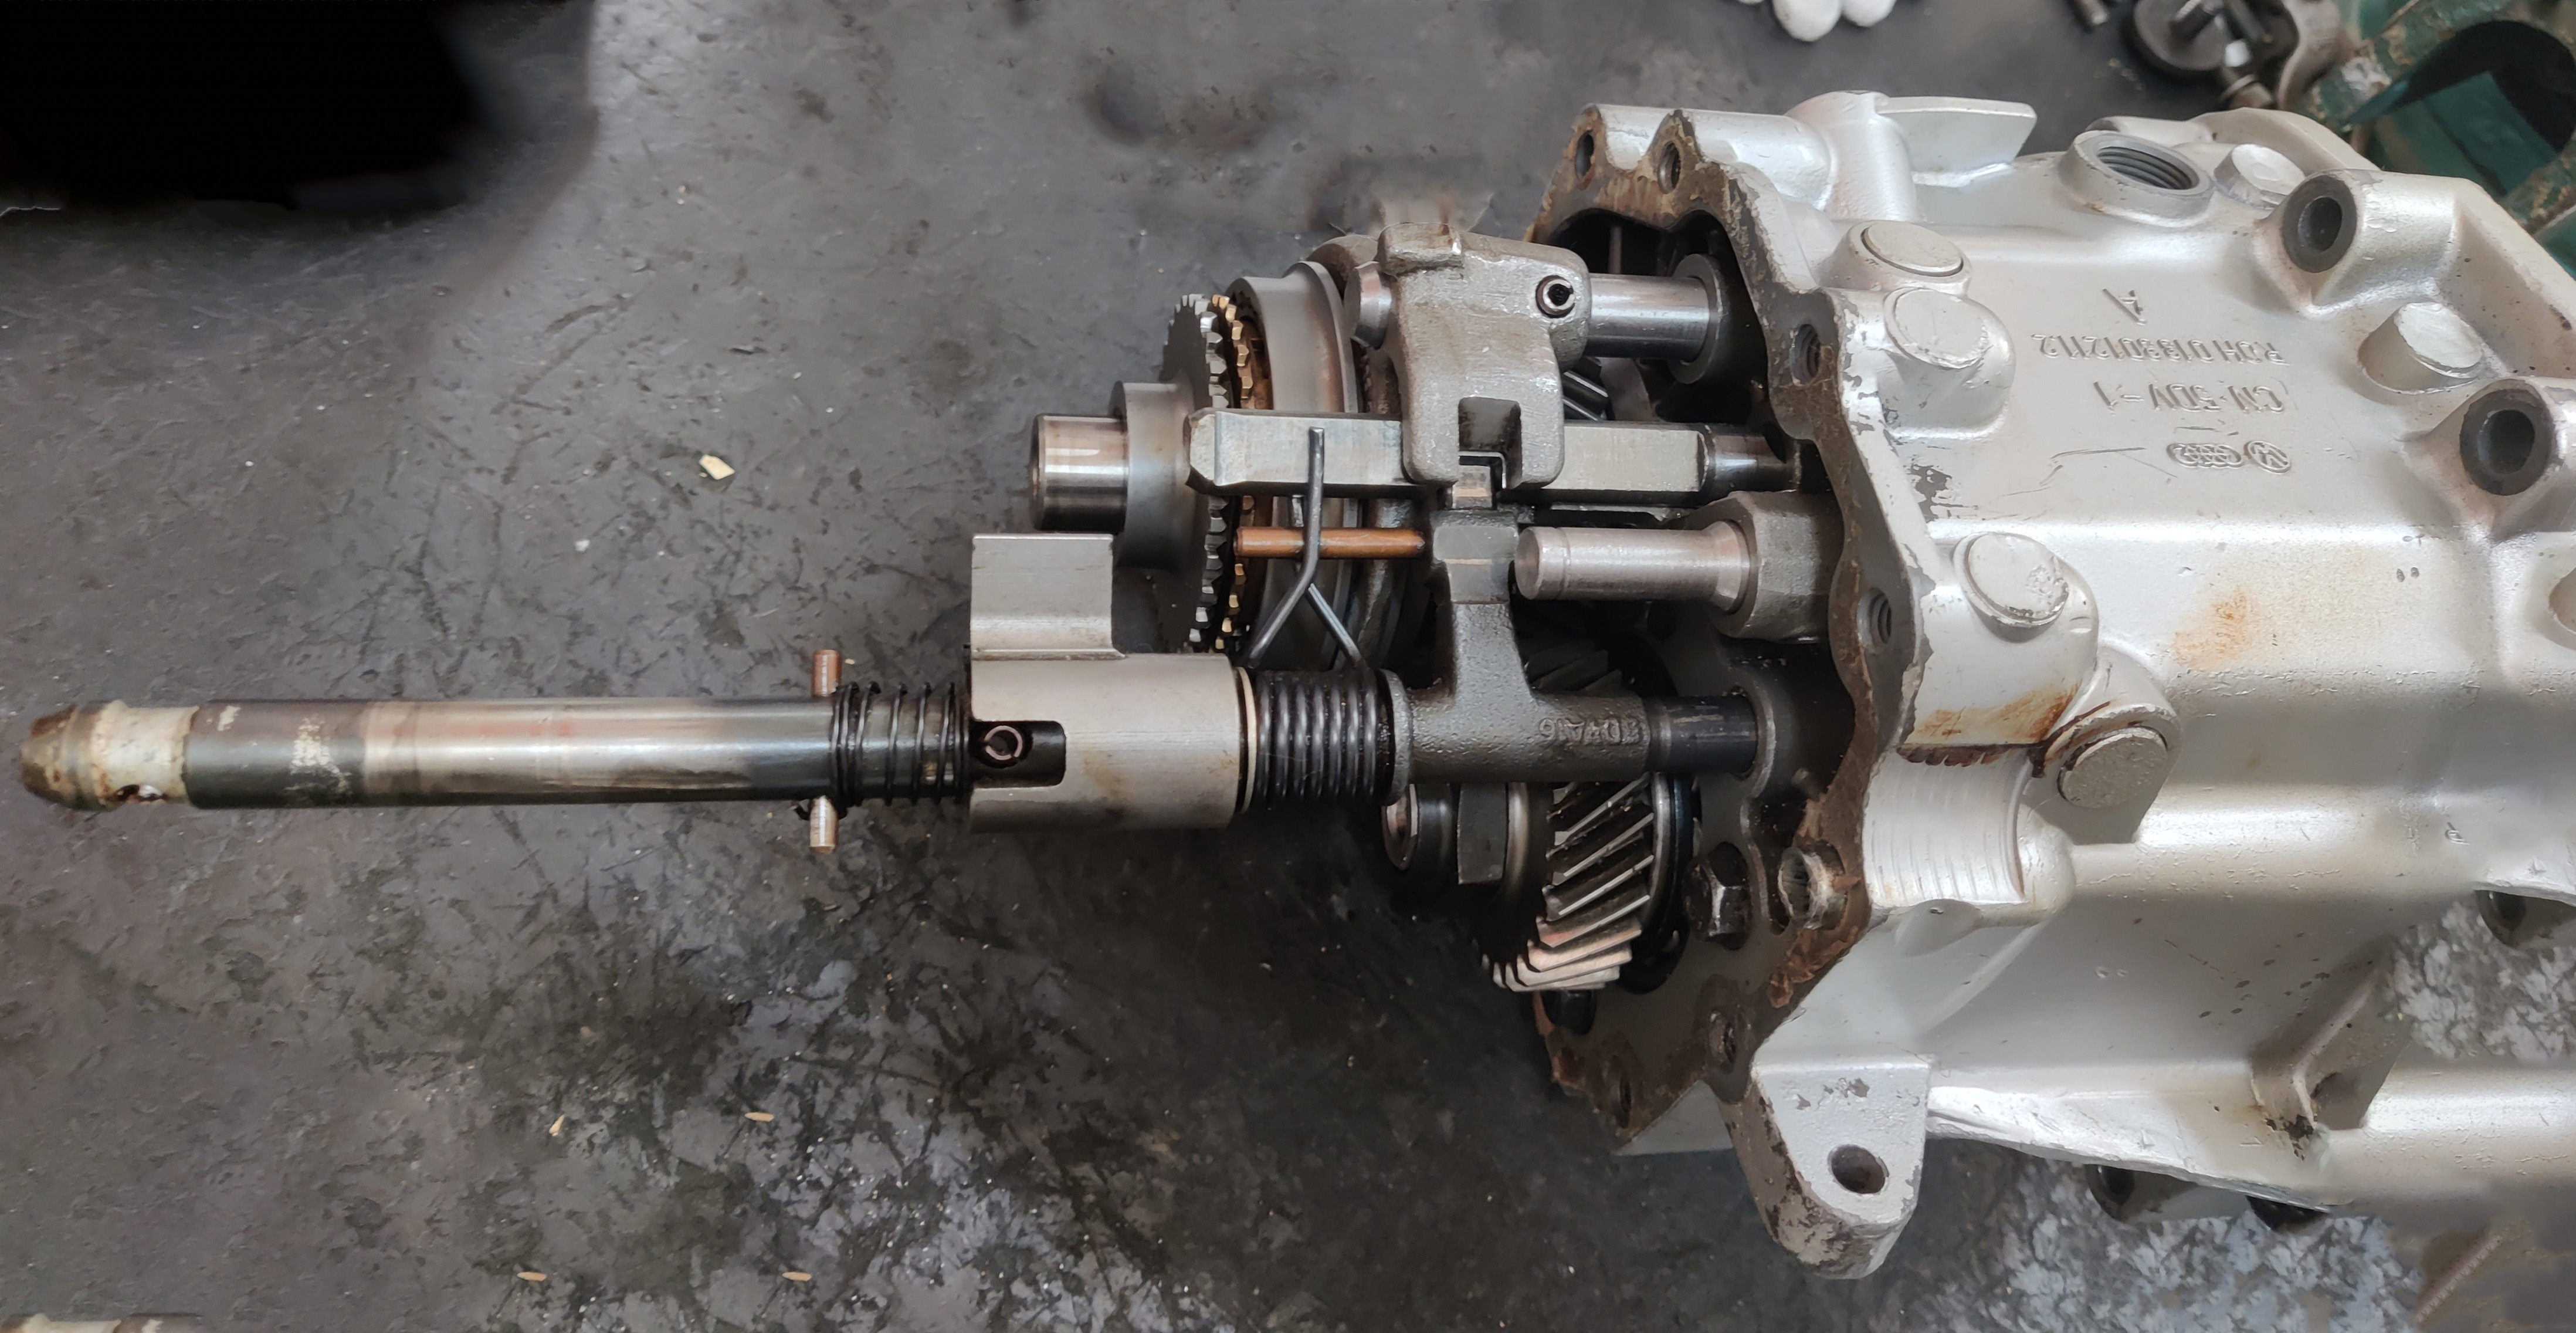
\includegraphics[width=\textwidth]{gearbox}
			\caption{变速器}
			\label{gearbox}
		\end{minipage}
		\begin{minipage}[b]{\textwidth}
			\centering
			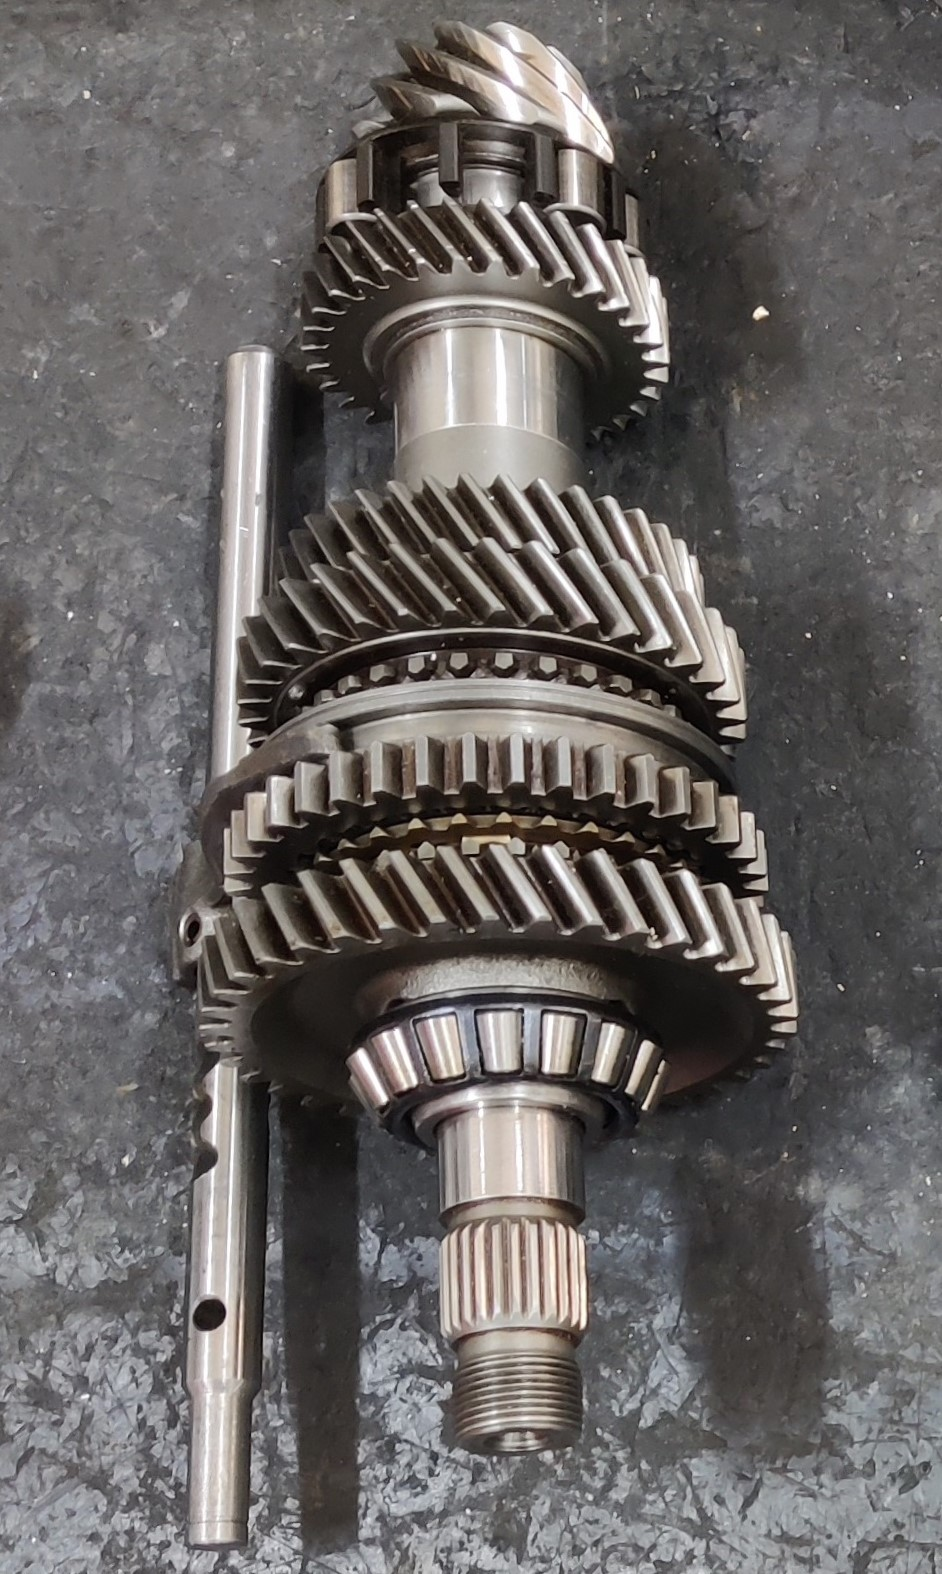
\includegraphics[width=\textwidth]{output shaft}
			\caption{输出轴}
			\label{output shaft}
		\end{minipage}
	\end{minipage}
	\begin{minipage}[b]{0.39\textwidth}
		\centering
		\begin{minipage}[b]{\textwidth}
			\centering
			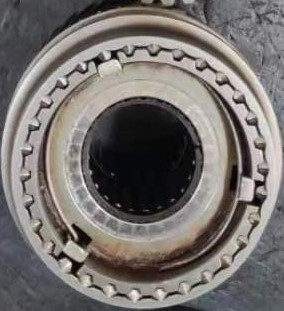
\includegraphics[width=\textwidth]{synchronous}
			\caption{同步器}
			\label{synchronous}
		\end{minipage}
		\begin{minipage}[b]{\textwidth}
			\centering
			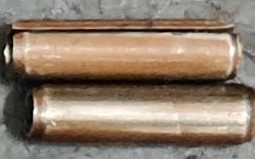
\includegraphics[width=\textwidth]{location pins}
			\caption{定位销}
			\label{location pins}
		\end{minipage}
	\end{minipage}
\end{figure}

\subsection{两轴变速器的工作原理。}

变速器的作用主要表现在三方面:第一,改变传动比,扩大驱动轮的转矩和转速的变化范围;第二,在发动机转向不变的情况下,实现汽车倒退行驶;第三,利用空挡,使得可以中断发动机动力传递,让发动机可以起动、怠速。

两轴式变速器的动力传递主要依靠两个相互平行的轴(输入轴和输出轴)完成,此外还有一根较短的倒挡轴帮助汽车实现倒退行驶。动力从第一轴输入,经一对齿轮传动后,直接由第二轴输出,故其在一般的减速挡时效率高于三轴式变速器,但无法设置高效的真正的直接挡,且输出轴转向和输入轴相反。

两轴式变速器的前进挡一般都采用常啮合斜齿轮,主动齿轮均为右旋,从动齿轮均为左旋,每对啮合斜齿轮中总有一个是空套在轴上。现在变速器的前进挡一般都采用同步器换挡,需换入某一工作挡位时拨动换挡杆,带动换挡滑块和拨叉将接合套与相应挡位空套的那个齿轮上的接合齿圈接合,使得该齿轮与输入轴或输出轴刚性连接,从而传递动力。各挡的动力传递路线已在\cref{subsection:2.1}中提到过。

为实现汽车的倒退行驶,在输入轴的一侧设置有一根较短的倒挡轴。倒挡中间齿轮空套在倒挡轴上(不用滚针轴承),可轴向滑动,空挡时与输入轴和输出轴的倒挡齿轮不在同一平面。我们在拆装实践中发现,该型变速器倒挡采用直齿滑动齿轮换挡,且输入轴倒挡齿轮、输出轴倒挡齿轮和倒挡中间齿轮在换挡时接合的那一侧都做了斜面处理,在换入倒挡时有一定的导向作用。显然换入倒挡前需先停车,故倒挡可不用接合套,拨动倒挡齿轮使其同时与输入、输出轴上两对应齿轮啮合即可。

两轴式变速器的结构简单、紧凑,容易布置,多用于前置前驱(FF)或后置后驱(RR)的普通级和中级轿车上。

\newpage

\section{汽油机部分}
\subsection{一般的配气机构、 进气门间隙和排气门间隙哪个气门间隙更大一些? 为什么?}
\subsection{曲柄连杆机构由哪些零件组成?}
\subsection{试述活塞环的分类与作用。}
\subsection{安装活塞环时应注意什么?}
\subsection{活塞、 连杆、 连杆盖组合装配时, 应注意什么?}
\subsection{绘制润滑系统或冷却系统原理示意图(二选一) ?}
\newpage

\section{柴油机部分}
\subsection{请简述柴油机工作原理}
\subsection{请简述柴油机与汽油机之间的区别}
\subsection{请简述柴油机的构造(按照机构逐项说明)}
\newpage

\section{汽车电子部分}
\subsection{简述 ABS 系统组成及工作原理。}
\subsection{以循环图示表述车载空调的工作原理, 并分析车载空调制冷与制热模式的区别。}
\subsection{电子车身稳定系统对车辆的意义,工作实现方式。}
\subsection{对于 ADAS 系统以及未来车辆电子化发展的感想。}
\newpage

\section{底盘部分}
\subsection{麦弗逊悬架中的减震器的轴线为什么和螺旋弹簧的轴线不重合?}
\subsection{多连杆悬架那些四轮定位定位参数可以调整,如何调整?}
\subsection{试叙述减振器的工作原理和几个功能阀的作用。}
\subsection{你拆有哪些类型的转向器?各有什么特点?如何调整转向系统间隙?}
\subsection{摩擦式离合器自由间隙的位置,并说出为什么要有自由间隙。自由间隙的过大过小有什
	么不利的影响? 车辆在使用过程中自由间隙是怎样变化的?}
\subsection{试述液力变矩器工作原理,其泵轮、导轮和涡轮分别与什么部件相连接?}
\subsection{简述鼓式制动器间隙自动调整原理。}
\subsection{简述真空助力泵的工作原理。}
\subsection{简述万向节的构造特性、 种类以及速度特性。}
\newpage


\end{document}